
%%%%%%%%%%%%%%%%%%%%%%%%%%%%%%%%%%%%%%%%%%%%%%%%%%%%%%%%%%%%%%%%%%%%%%
%%%%%%%%%%%%%%%%%%%%%%%%%%%%%%%%%%%%%%%%%%%%%%%%%%%%%%%%%%%%%%%%%%%%%
%%%%%%%%%%%%%%%%%%%%%%%%%%%%%%%%%%%%%%%%%%%%%%%%%%%%%%%%%%%%%%%%%%%%%
%%%%%%%%%%%%%%%%%%%%%%%%%%%%%%%%%%%%%%%%%%%%%%%%%%%%%%%%%%%%%%%%%%%%%

\chapter{Distributions in ProbOnto knowledge base}
\label{ch:probontoAppendix}

The full first version of ProbOnto will be released soon. Here we provide 
a quite detailed overview of its content for the currently about 66 distributions
or alternative parameterisations. The according plots have been performed using 
the R code stored in ProbOnto and provided for each distribution for which it's available.


%%%%%%%%%%%%%%%%%%%%%%%%%%%%%%%%%%%%%%%%%%%%%%%%%%%%%%%%%%%%%%%%%%%%%
\section{Symbols}
Some of the symbols used in definitions of the functions and quantities 
listed in the subsequent sections are collected here with references
\begin{itemize}
\item Beta function, $B(x,y)$\\
\begin{equation*}
B(x,y) = \frac{\Gamma(x)\Gamma(y)}{\Gamma(x+y)}
\end{equation*}
\url{mathworld.wolfram.com/BetaFunction.html}\\
\url{en.wikipedia.org/wiki/Beta_function}
\item Regularized incomplete Beta function,  $I_p(a,b)$, $I_{1-p}(a,b)$\\
\begin{equation*}
I_x(a,b) = \frac{B(x;a,b)}{B(a,b)}
\end{equation*}
with
\begin{equation*}
B(x;a,b) = \int_0^x t^{a-1} (1-t)^{b-1} dt
\end{equation*}
then \emph{incomplete beta function}.\\
\url{mathworld.wolfram.com/RegularizedBetaFunction.html}\\
\url{en.wikipedia.org/wiki/Beta_function#Incomplete_beta_function}
\item Error function, $erf$\\
\begin{equation*}
\text{erf}(z) = \frac{2}{\pi}\int_0^z e^{-t^2} dt
\end{equation*}
\url{mathworld.wolfram.com/Erf.html}\\
\url{en.wikipedia.org/wiki/Error_function}
\item Floor function, $\lfloor x \rfloor$\\
\begin{equation*}
\text{floor}(x) = \lfloor x\rfloor \text{ is the largest integer not greater than } x 
\end{equation*}
\url{mathworld.wolfram.com/FloorFunction.html}\\
\url{en.wikipedia.org/wiki/Floor_and_ceiling_functions}
\item Gamma function, $\Gamma$ \\
\begin{equation*}
\Gamma(n) = (n-1)!, \text{ for } n - \text{ positive integer}
\end{equation*}
\url{mathworld.wolfram.com/GammaFunction.html}\\
\url{en.wikipedia.org/wiki/Gamma_function}
\item Lower incomplete gamma function, $\gamma$\\
\begin{equation*}
  \gamma(s,x) = \int_0^x t^{s-1}\,e^{-t}\,{\rm d}t
\end{equation*}
\url{mathworld.wolfram.com/IncompleteGammaFunction.html}\\
\url{en.wikipedia.org/wiki/Incomplete_gamma_function}
\item Multivariate Gamma function,	$\Gamma_p$\\
\begin{equation*}
\Gamma_p(a)= \pi^{p(p-1)/4}\prod_{j=1}^p \Gamma\left[ a+(1-j)/2\right]
\end{equation*}
\url{en.wikipedia.org/wiki/Multivariate_gamma_function}
\item Iverson bracket, $[x=i]$\\ 
\begin{equation*}
[P] = \begin{cases} 1 & \text{if } P \text{ is true;} \\ 0 & \text{otherwise.} \end{cases}
\end{equation*}
\url{mathworld.wolfram.com/IversonBracket.html}\\
\url{en.wikipedia.org/wiki/Iverson_bracket}
%\item Linear span, $span$\\
%\url{mathworld.wolfram.com/VectorSpaceSpan.html}\\
%\url{en.wikipedia.org/wiki/Linear_span}
\item Generalized Hypergeometric function, ${}_pF_q$\\
\begin{equation*}
{}_pF_q(a_1,\ldots,a_p;b_1,\ldots,b_q;z) = \sum_{n=0}^\infty \frac{(a_1)_n\dots(a_p)_n}{(b_1)_n\dots(b_q)_n} \, \frac {z^n} {n!}
\end{equation*}
\url{en.wikipedia.org/wiki/Generalized_hypergeometric_function}
\item Hypergeometric function, $_2F_1$\\
\begin{equation*}
{}_2F_1(a,b;c;z) = \sum_{n=0}^\infty \frac{(a)_n (b)_n}{(c)_n} \frac{z^n}{n!}.
\end{equation*}
\url{mathworld.wolfram.com/HypergeometricFunction.html}\\
\url{en.wikipedia.org/wiki/Hypergeometric_function}
\end{itemize}

\section{Distributions and their features}

\section*{Bernoulli} 

  \bigskip 

\begin{tabular}{p{2cm}cl}
\textbf{name} & & Bernoulli (ID: 0000000)\\ 
 
\textbf{type} & & discrete \\ 

\textbf{variate} & & $k$, scalar \\ 

\textbf{support} & & $k \in \{0,1\}$
\end{tabular}

\begin{figure}[ht!]
\centering
  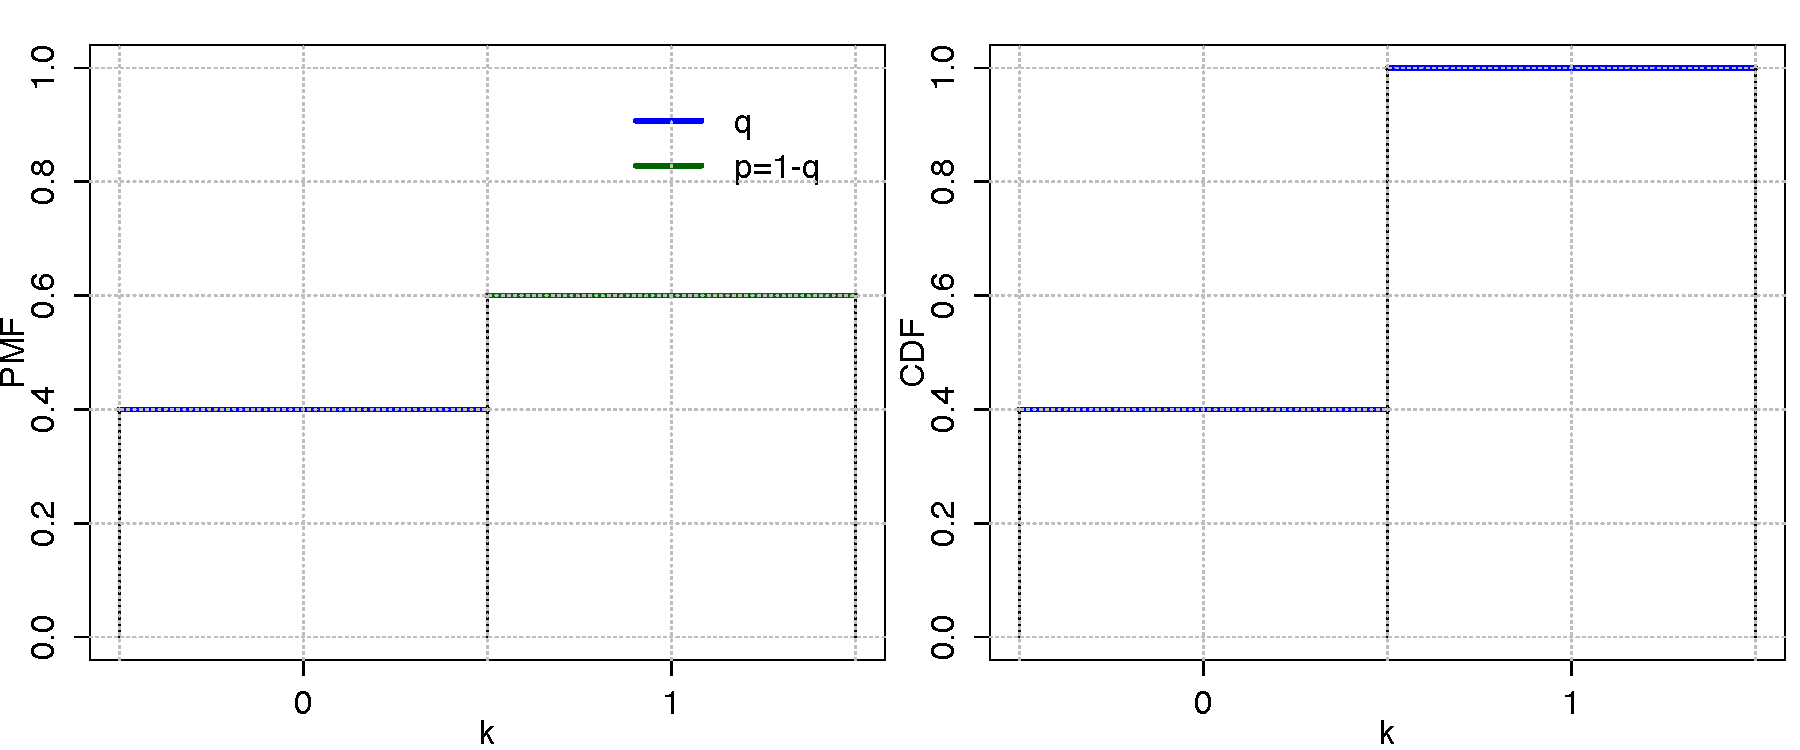
\includegraphics[width=140mm]{pics/Bernoulli.pdf}
 \caption{Bernoulli distribution plotted using the provided R code.}
 \label{fig:Bernoulli}
\end{figure}

\subsubsection*{Parameter: probability}

\noindent\begin{tabular}{p{2cm}cl}
\textbf{name} & & probability \\
\textbf{type} & & scalar \\
\textbf{symbol} & & $p$  \\
\textbf{definition} & & $0<p<1, p \in  R$
\end{tabular}
\subsubsection*{Functions}

\smallskip \noindent \hspace{.2cm} \textbf{PMF} 
\begin{equation*}\begin{cases}
    q=(1-p) & \text{for }k=0 \\ p & \text{for }k=1
    \end{cases}\end{equation*}
\smallskip \noindent \hspace{.2cm} \textbf{PMF in R}  
\begin{verbatim}q=(1-p) for k=0 \\
p for k=1\end{verbatim}
\smallskip \noindent \hspace{.2cm} \textbf{CDF} 
\begin{equation*}\begin{cases}
    0 & \text{for }k<0 \\ q & \text{for }0\leq k<1 \\ 1 & \text{for }k\geq 1
    \end{cases}\end{equation*}
\smallskip
\subsubsection*{Characteristics}
\smallskip \noindent \hspace{.2cm} \textbf{Mean} 
\begin{equation*}p\end{equation*}
\smallskip \noindent \hspace{.2cm} \textbf{Median} 
\begin{equation*}\begin{cases}
0 & \text{if } q > p\\
0.5 & \text{if } q=p\\
1 & \text{if } q<p
\end{cases}\end{equation*}
\smallskip \noindent \hspace{.2cm} \textbf{Mode} 
\begin{equation*}\begin{cases}
0 & \text{if } q > p\\
0, 1 & \text{if } q=p\\
1 & \text{if } q < p
\end{cases}\end{equation*}
\smallskip \noindent \hspace{.2cm} \textbf{Variance} 
\begin{equation*}p(1-p)\end{equation*}
\smallskip
\section*{Beta1} 

  \bigskip 

\begin{tabular}{p{2cm}cl}
\textbf{name} & & Beta (ID: 0000014)\\ 
 
\textbf{type} & & continuous \\ 

\textbf{variate} & & $x$, scalar \\ 

\textbf{support} & & $x \in (0,1)$
\end{tabular}

\begin{figure}[ht!]
\centering
  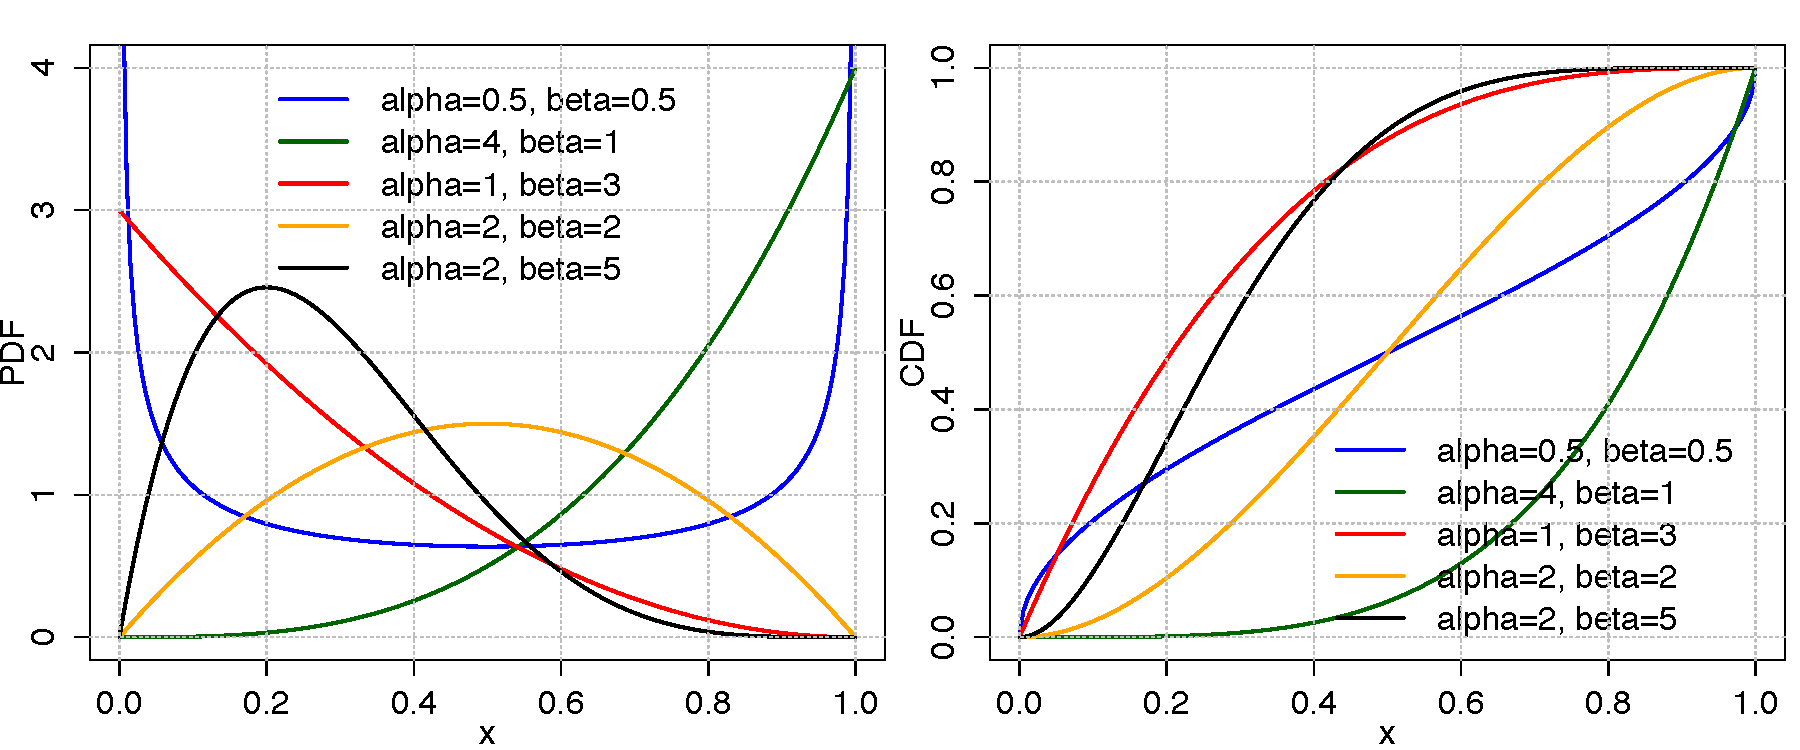
\includegraphics[width=140mm]{pics/Beta.pdf}
 \caption{Beta distribution plotted using the provided R code.}
 \label{fig:Beta}
\end{figure}

\subsubsection*{Parameter: alpha}

\noindent\begin{tabular}{p{2cm}cl}
\textbf{name} & & shape \\
\textbf{type} & & scalar \\
\textbf{symbol} & & $\alpha$  \\
\textbf{definition} & & $\alpha > 0$
\end{tabular}
\subsubsection*{Parameter: beta}

\noindent\begin{tabular}{p{2cm}cl}
\textbf{name} & & shape \\
\textbf{type} & & scalar \\
\textbf{symbol} & & $\beta$  \\
\textbf{definition} & & $\beta > 0$
\end{tabular}
\subsubsection*{Functions}

\smallskip \noindent \hspace{.2cm} \textbf{PDF} 
\begin{equation*}\frac{x^{\alpha-1}(1-x)^{\beta-1}} {B(\alpha,\beta)} \end{equation*}
\smallskip \noindent \hspace{.2cm} \textbf{PDF in R}  
\begin{verbatim}(x^(alpha-1)*(1-x)^(beta-1))/beta(alpha,beta)\end{verbatim}
\smallskip \noindent \hspace{.2cm} \textbf{CDF} 
\begin{equation*}I_x(\alpha,\beta)\end{equation*}
\smallskip \noindent \hspace{.2cm} \textbf{CDF in R} 
\begin{verbatim}Rbeta(x, a, b)\end{verbatim}
\smallskip
\subsubsection*{Characteristics}
\smallskip \noindent \hspace{.2cm} \textbf{Mean} 
\begin{equation*}\frac{\alpha}{\alpha+\beta}\end{equation*}
\smallskip \noindent \hspace{.2cm} \textbf{Median} 
\begin{equation*}I_{\frac{1}{2}}^{[-1]}(\alpha,\beta)\end{equation*}
\smallskip \noindent \hspace{.2cm} \textbf{Mode} 
\begin{equation*}\frac{\alpha-1}{\alpha+\beta-2}\end{equation*}
\smallskip \noindent \hspace{.2cm} \textbf{Variance} 
\begin{equation*}\frac{\alpha\beta}{(\alpha+\beta)^2(\alpha+\beta+1)}\end{equation*}
\smallskip
\section*{Binomial1} 

  \bigskip 

\begin{tabular}{p{2cm}cl}
\textbf{name} & & Binomial (ID: 0000027)\\ 
 
\textbf{type} & & discrete \\ 

\textbf{variate} & & $k$, scalar \\ 

\textbf{support} & & $k \in \{0,\dots,n\}$
\end{tabular}

\begin{figure}[ht!]
\centering
  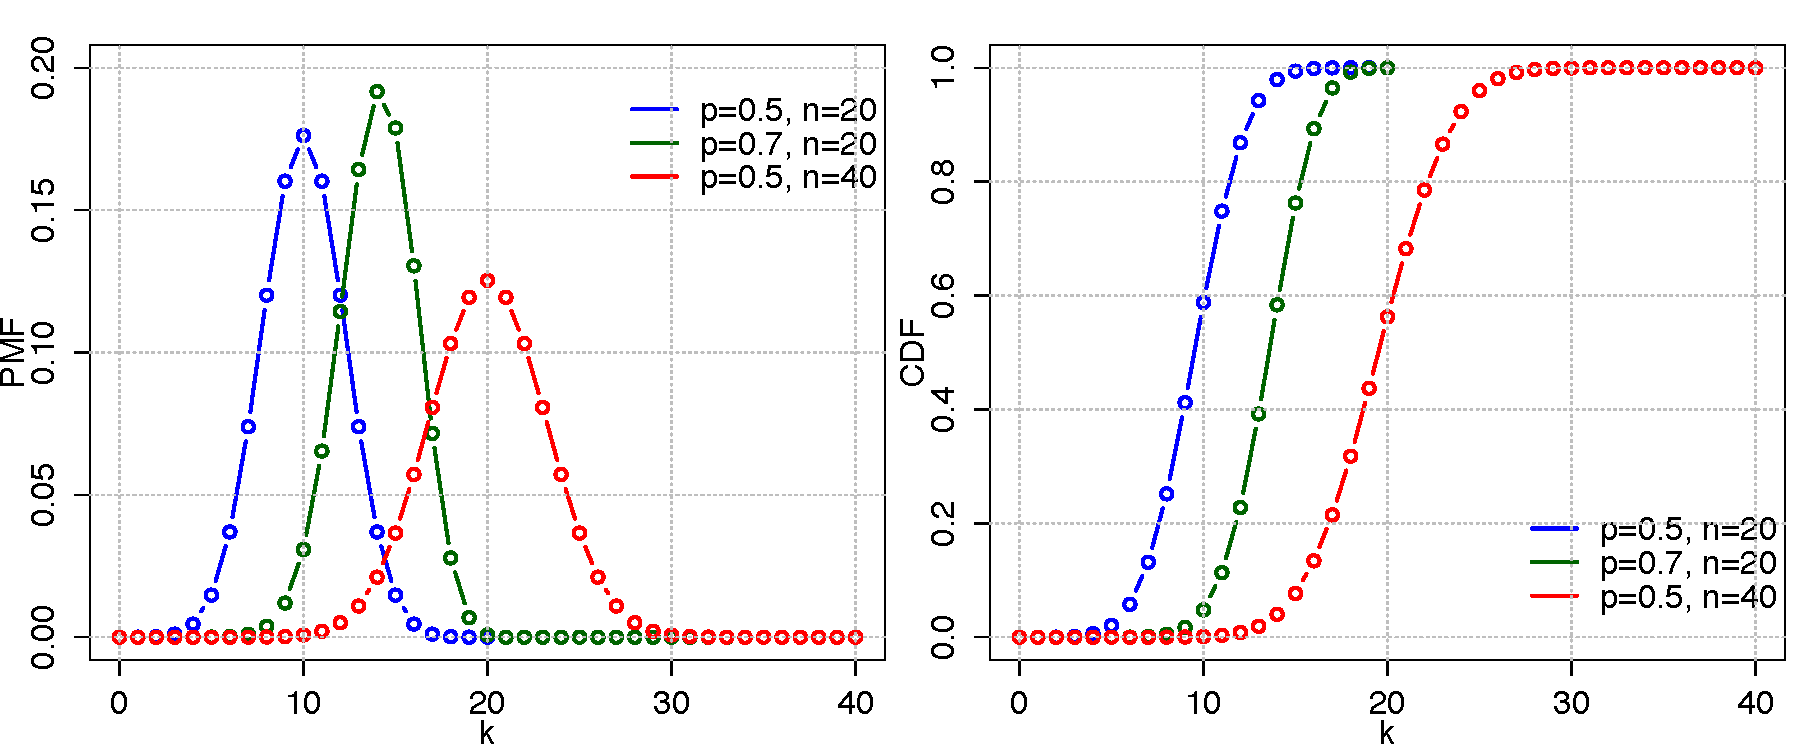
\includegraphics[width=140mm]{pics/Binomial.pdf}
 \caption{Binomial distribution plotted using the provided R code.}
 \label{fig:Binomial}
\end{figure}

\subsubsection*{Parameter: numberOfFailures}

\noindent\begin{tabular}{p{2cm}cl}
\textbf{name} & & number of trials \\
\textbf{type} & & scalar \\
\textbf{symbol} & & $n$  \\
\textbf{definition} & & $n \in N, n \ge 0$
\end{tabular}
\subsubsection*{Parameter: probability}

\noindent\begin{tabular}{p{2cm}cl}
\textbf{name} & & success probability in each trial \\
\textbf{type} & & scalar \\
\textbf{symbol} & & $p$  \\
\textbf{definition} & & $p \in [0,1]$
\end{tabular}
\subsubsection*{Functions}

\smallskip \noindent \hspace{.2cm} \textbf{PMF} 
\begin{equation*}{n \choose k}\, p^k (1-p)^{n-k}\end{equation*}
\smallskip \noindent \hspace{.2cm} \textbf{PMF in R}  
\begin{verbatim}choose(n,k) * p^k*(1-p)^(n-k)\end{verbatim}
\smallskip \noindent \hspace{.2cm} \textbf{CDF} 
\begin{equation*}I_{1-p}(n - k, 1 + k)\end{equation*}
\smallskip \noindent \hspace{.2cm} \textbf{CDF in R} 
\begin{verbatim}Rbeta(1-p, n-k, 1+k)\end{verbatim}
\smallskip
\subsubsection*{Characteristics}
\smallskip \noindent \hspace{.2cm} \textbf{Mean} 
\begin{equation*}np\end{equation*}
\smallskip \noindent \hspace{.2cm} \textbf{Median} 
\begin{equation*}\lfloor np \rfloor \text{ or } \lceil np \rceil\end{equation*}
\smallskip \noindent \hspace{.2cm} \textbf{Mode} 
\begin{equation*}\lfloor (n + 1)p \rfloor \; or \; \lfloor (n + 1)p \rfloor - 1\end{equation*}
\smallskip \noindent \hspace{.2cm} \textbf{Variance} 
\begin{equation*}np(1 - p)\end{equation*}
\smallskip
\section*{BirnbaumSaunders1} 

  \bigskip 

\begin{tabular}{p{2cm}cl}
\textbf{name} & & Birnbaum-Saunders (ID: 0000039)\\ 
 
\textbf{type} & & continuous \\ 

\textbf{variate} & & $x$, scalar \\ 

\textbf{support} & & $x \in (0,+\infty)$
\end{tabular}

\begin{figure}[ht!]
\centering
  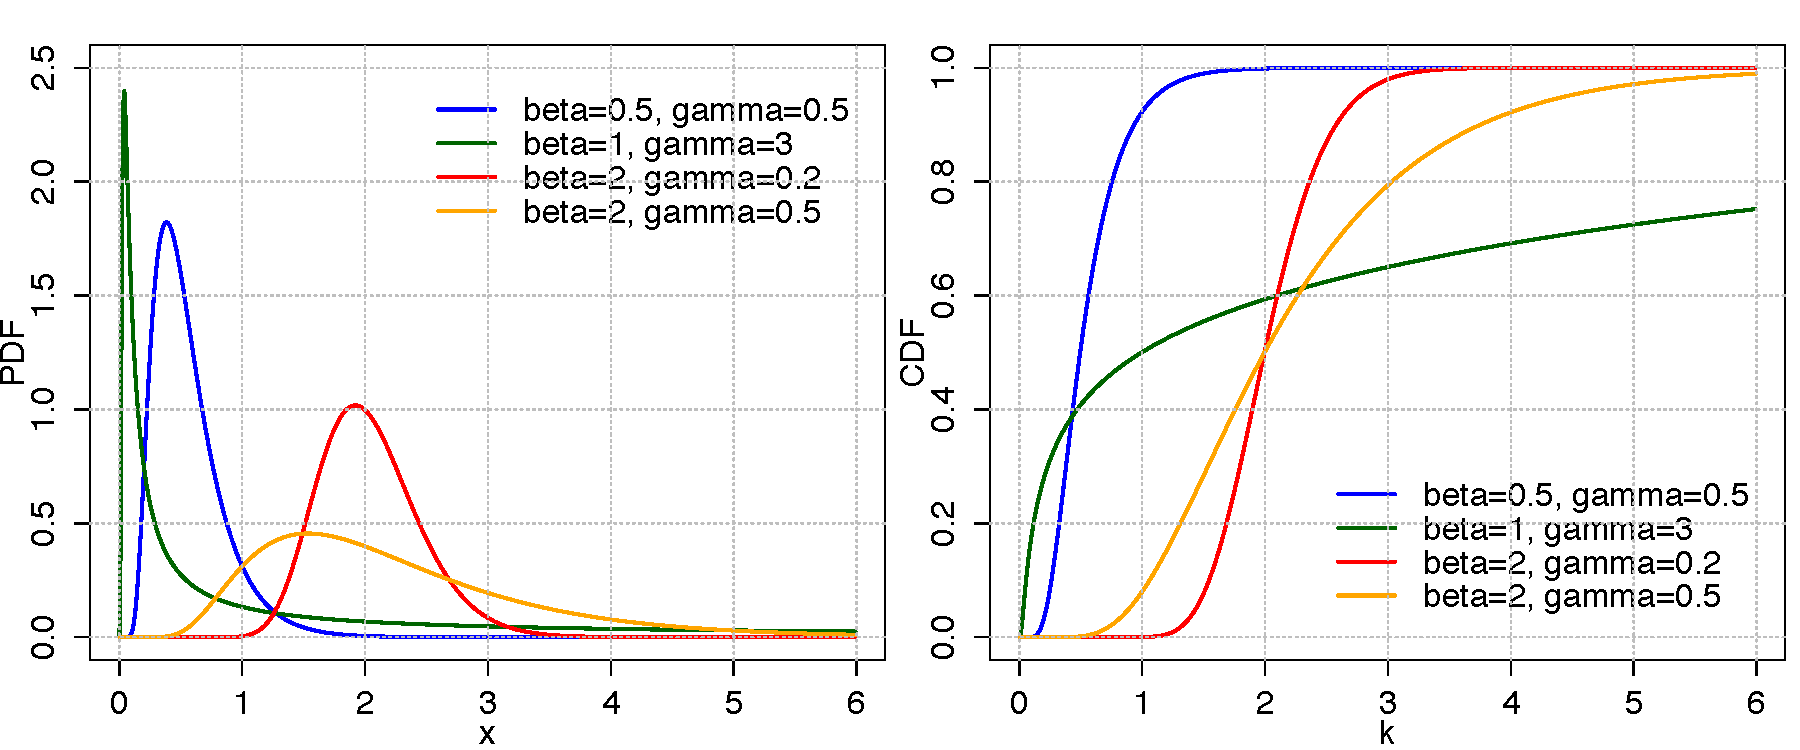
\includegraphics[width=140mm]{pics/BirnbaumSaunders.pdf}
 \caption{BirnbaumSaunders distribution plotted using the provided R code.}
 \label{fig:BirnbaumSaunders}
\end{figure}

\subsubsection*{Parameter: scale}

\noindent\begin{tabular}{p{2cm}cl}
\textbf{name} & & scale \\
\textbf{type} & & scalar \\
\textbf{symbol} & & $\beta$  \\
\textbf{definition} & & $\beta > 0$
\end{tabular}
\subsubsection*{Parameter: shape}

\noindent\begin{tabular}{p{2cm}cl}
\textbf{name} & & shape \\
\textbf{type} & & scalar \\
\textbf{symbol} & & $\gamma$  \\
\textbf{definition} & & $\gamma > 0$
\end{tabular}
\subsubsection*{Functions}

\smallskip \noindent \hspace{.2cm} \textbf{PDF} 
\begin{equation*}\frac{1}{\sqrt{2\pi}}\exp\Big[-\frac{(\sqrt{x/\beta}-\sqrt{\beta/x})^2}{2\gamma^2}\Big]\Big[\frac{\sqrt{x/\beta}+\sqrt{\beta/x}}{2\gamma x}\Big]\end{equation*}
\smallskip \noindent \hspace{.2cm} \textbf{PDF in R}  
\begin{verbatim}PDF=1/(sqrt(2*pi))
*exp(-(sqrt(x/beta)-sqrt(beta/x))^2/(2*gamma^2))*(sqrt(x/beta)+sqrt(beta/x))/(2*gamma*x)
\end{verbatim}
\smallskip \noindent \hspace{.2cm} \textbf{CDF} 
\begin{equation*}\int_0^x f(x),
\text { with f the PDF}\end{equation*}
\smallskip \noindent \hspace{.2cm} \textbf{CDF in R}  
\begin{verbatim}
cumsum(PDF*rep(stepSize,length(PDF)))
\end{verbatim}
\smallskip
\subsubsection*{Characteristics}
\smallskip
\section*{CategoricalNonordered1} 

  \bigskip 

\begin{tabular}{p{2cm}cl}
\textbf{name} & & Categorical Nonordered (ID: 0000058)\\ 
 
\textbf{type} & & discrete \\ 

\textbf{variate} & & $x$, scalar \\ 

\textbf{support} & & $x \in \{1,\dots,k\}$
\end{tabular}

\begin{figure}[ht!]
\centering
  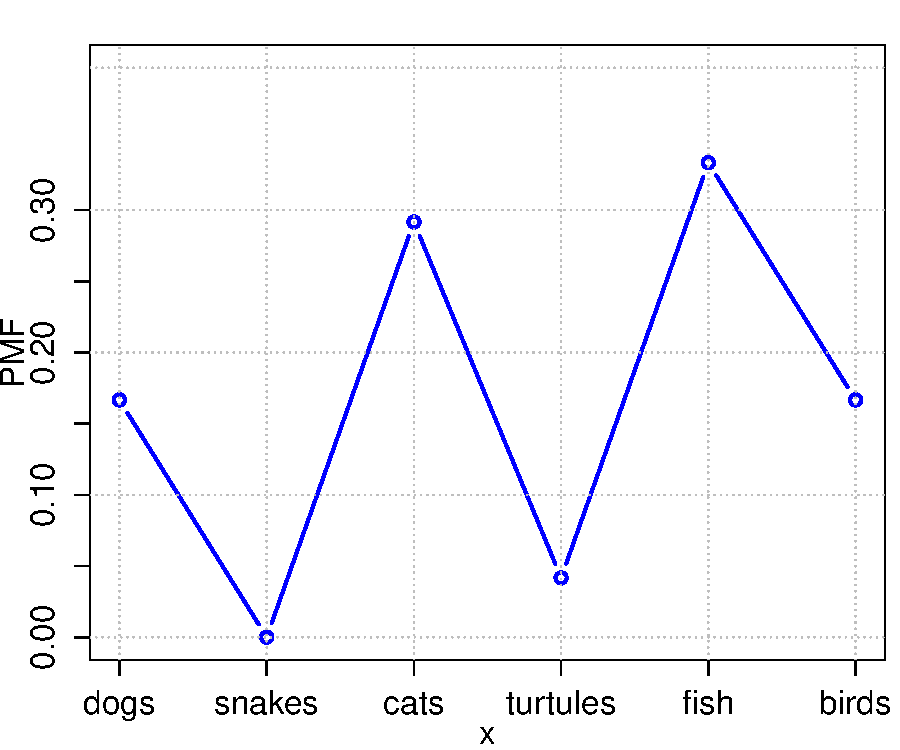
\includegraphics[width=70mm]{pics/CategoricalNonordered.pdf}
 \caption{CategoricalNonordered distribution plotted using the provided R code.}
 \label{fig:CategoricalNonordered}
\end{figure}

\subsubsection*{Parameter: categoryProb}

\noindent\begin{tabular}{p{2cm}cl}
\textbf{name} & & category probabilities \\
\textbf{type} & & vector \\
\textbf{symbol} & & $p_1, \ldots, p_k$  \\
\textbf{definition} & & $0 \leq p_i \leq 1, \Sigma p_i = 1$
\end{tabular}
\subsubsection*{Functions}

\smallskip \noindent \hspace{.2cm} \textbf{PMF} 
\begin{equation*}p(x=i)=p_i\end{equation*}
\smallskip \noindent \hspace{.2cm} \textbf{CDF} 
\begin{equation*}undefined\end{equation*}
\smallskip
\subsubsection*{Characteristics}
\smallskip \noindent \hspace{.2cm} \textbf{Mean} 
\begin{equation*}E([x=i]) = p_i, \text{this is the mean of the Iverson bracket } [x=i] \text{ and not the mean of } x\end{equation*}
\smallskip \noindent \hspace{.2cm} \textbf{Median} 
\begin{equation*}i\text{ such that }\sum_{j=1}^{i-1} p_j \leq 0.5\text{ and }\sum_{j=1}^{i} p_j \geq 0.5\end{equation*}
\smallskip \noindent \hspace{.2cm} \textbf{Mode} 
\begin{equation*}i\text{ such that }p_i=\max(p_1, \ldots, p_k)\end{equation*}
\smallskip \noindent \hspace{.2cm} \textbf{Variance} 
\begin{align*}
Var([x=i]) &= p_i (1-p_i) \\ 
Cov([x=i],[x=j]) &= - p_i p_j~~(i\neq j)\end{align*}
\smallskip
\section*{CategoricalOrdered1} 

  \bigskip 

\begin{tabular}{p{2cm}cl}
\textbf{name} & & Categorical Ordered (ID: 0000049)\\ 
 
\textbf{type} & & discrete \\ 

\textbf{variate} & & $x$, scalar \\ 

\textbf{support} & & $x \in \{1,\dots,k\}$
\end{tabular}

\begin{figure}[ht!]
\centering
  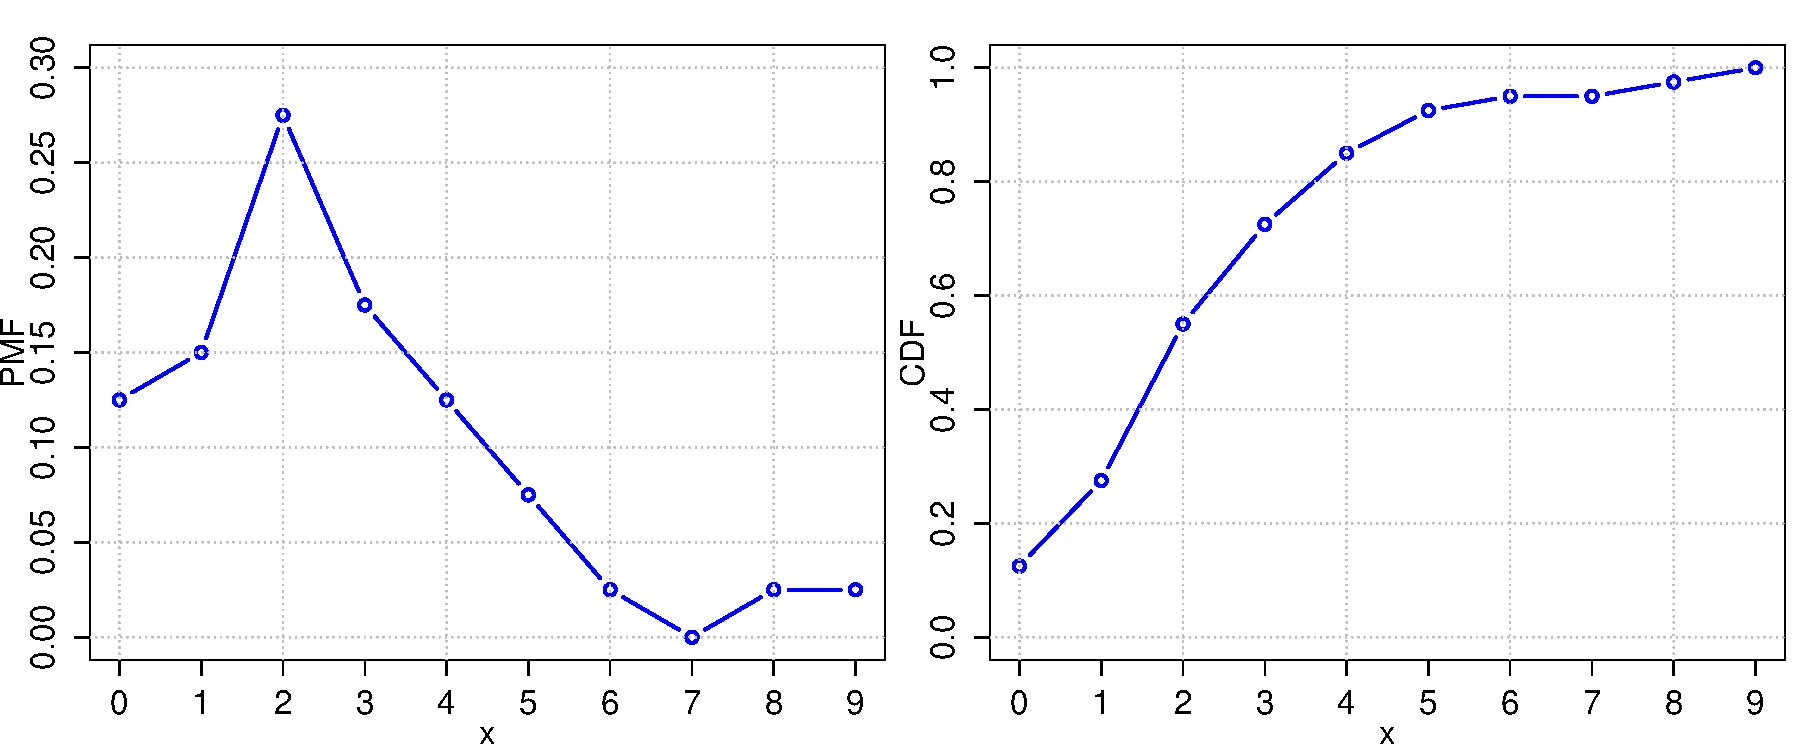
\includegraphics[width=140mm]{pics/CategoricalOrdered.pdf}
 \caption{CategoricalOrdered distribution plotted using the provided R code.}
 \label{fig:CategoricalOrdered}
\end{figure}

\subsubsection*{Parameter: categoryProb}

\noindent\begin{tabular}{p{2cm}cl}
\textbf{name} & & category probabilities \\
\textbf{type} & & vector \\
\textbf{symbol} & & $p_1, \ldots, p_k$  \\
\textbf{definition} & & $0 \leq p_i \leq 1, \Sigma p_i = 1$
\end{tabular}
\subsubsection*{Functions}

\smallskip \noindent \hspace{.2cm} \textbf{PMF} 
\begin{equation*}p(x=i)=p_i\end{equation*}
\smallskip \noindent \hspace{.2cm} \textbf{CDF} 
\begin{equation*}\begin{cases}
    0 & \text{for }x<1 \\
    \sum_{j=1}^i p_j & \text{for }x \in [i,i+1) \\
    1 & \text{for }x \geq k
    \end{cases}\end{equation*}
\smallskip
\subsubsection*{Characteristics}
\smallskip \noindent \hspace{.2cm} \textbf{Mean} 
\begin{equation*}E([x=i]) = p_i, \text{this is the mean of the Iverson bracket } [x=i] \text{ and not the mean of } x\end{equation*}
\smallskip \noindent \hspace{.2cm} \textbf{Median} 
\begin{equation*}i\text{ such that }\sum_{j=1}^{i-1} p_j \leq 0.5\text{ and }\sum_{j=1}^{i} p_j \geq 0.5\end{equation*}
\smallskip \noindent \hspace{.2cm} \textbf{Mode} 
\begin{equation*}i\text{ such that }p_i=\max(p_1, \ldots, p_k)\end{equation*}
\smallskip \noindent \hspace{.2cm} \textbf{Variance} 
\begin{align*}Var([x=i]) &= p_i (1-p_i) \\ Cov([x=i],[x=j]) &= - p_i p_j~~(i\neq j)\end{align*}
\smallskip
\section*{Cauchy1} 

  \bigskip 

\begin{tabular}{p{2cm}cl}
\textbf{name} & & Cauchy (ID: 0000067)\\ 
 
\textbf{type} & & continuous \\ 

\textbf{variate} & & $x$, scalar \\ 

\textbf{support} & & $x \in (-\infty,+\infty)$
\end{tabular}

\begin{figure}[ht!]
\centering
  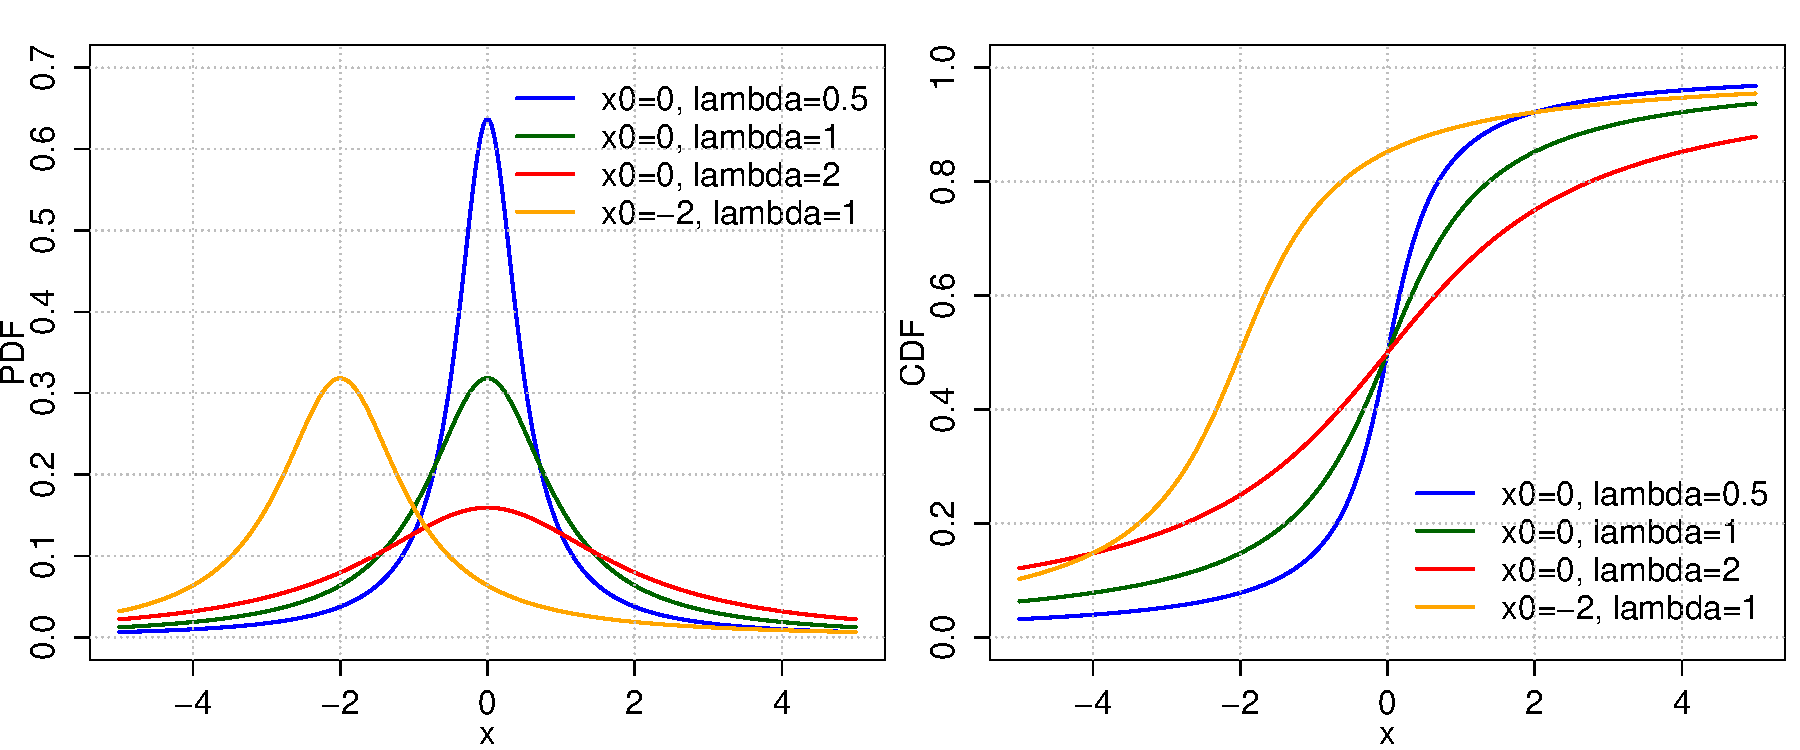
\includegraphics[width=140mm]{pics/Cauchy.pdf}
 \caption{Cauchy distribution plotted using the provided R code.}
 \label{fig:Cauchy}
\end{figure}

\subsubsection*{Parameter: location}

\noindent\begin{tabular}{p{2cm}cl}
\textbf{name} & & location \\
\textbf{type} & & scalar \\
\textbf{symbol} & & $x_0$  \\
\textbf{definition} & & $x_0 \in  R$
\end{tabular}
\subsubsection*{Parameter: scale}

\noindent\begin{tabular}{p{2cm}cl}
\textbf{name} & & scale \\
\textbf{type} & & scalar \\
\textbf{symbol} & & $\gamma$  \\
\textbf{definition} & & $\gamma \in  R$
\end{tabular}
\subsubsection*{Functions}

\smallskip \noindent \hspace{.2cm} \textbf{PDF} 
\begin{equation*}\frac{1}{\pi\gamma\,\left[1 + \left(\frac{x-x_0}{\gamma}\right)^2\right]}\end{equation*}
\smallskip \noindent \hspace{.2cm} \textbf{PDF in R}  
\begin{verbatim}1 / (pi*gamma*(1 + ((x-x0)^2/gamma^2)))\end{verbatim}
\smallskip \noindent \hspace{.2cm} \textbf{CDF} 
\begin{equation*}\frac{1}{\pi} \arctan\left(\frac{x-x_0}{\gamma}\right)+\frac{1}{2}\end{equation*}
\smallskip \noindent \hspace{.2cm} \textbf{CDF in R} 
\begin{verbatim}1/pi * atan((x-x0)/gamma)+1/2\end{verbatim}
\smallskip
\subsubsection*{Characteristics}
\smallskip \noindent \hspace{.2cm} \textbf{Mean} 
\begin{equation*}undefined\end{equation*}
\smallskip \noindent \hspace{.2cm} \textbf{Median} 
\begin{equation*}x_0\end{equation*}
\smallskip \noindent \hspace{.2cm} \textbf{Mode} 
\begin{equation*}x_0\end{equation*}
\smallskip \noindent \hspace{.2cm} \textbf{Variance} 
\begin{equation*}undefined\end{equation*}
\smallskip
\section*{ChiSquared1} 

  \bigskip 

\begin{tabular}{p{2cm}cl}
\textbf{name} & & Chi-squared (ID: 0000077)\\ 
 
\textbf{type} & & continuous \\ 

\textbf{variate} & & $x$, scalar \\ 

\textbf{support} & & $x \in [0,+\infty)$
\end{tabular}

\begin{figure}[ht!]
\centering
  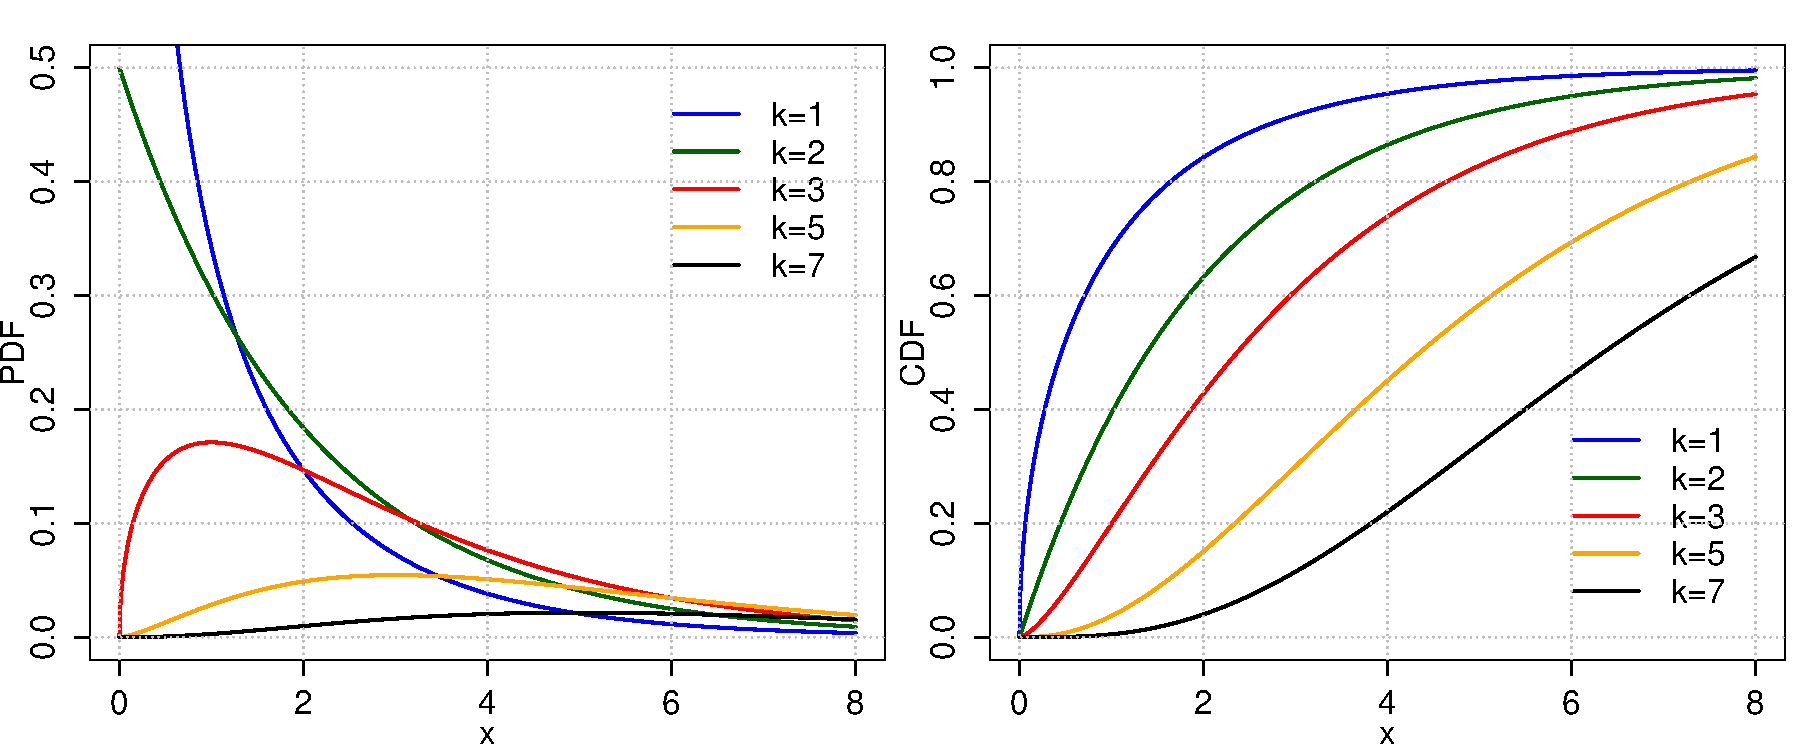
\includegraphics[width=140mm]{pics/ChiSquared.pdf}
 \caption{ChiSquared distribution plotted using the provided R code.}
 \label{fig:ChiSquared}
\end{figure}

\subsubsection*{Parameter: degreesOfFreedom}

\noindent\begin{tabular}{p{2cm}cl}
\textbf{name} & & degrees of freedom \\
\textbf{type} & & scalar \\
\textbf{symbol} & & $k$  \\
\textbf{definition} & & $k \in N$
\end{tabular}
\subsubsection*{Functions}

\smallskip \noindent \hspace{.2cm} \textbf{PDF} 
\begin{equation*}\frac{1}{2^{\frac{k}{2}}\Gamma\left(\frac{k}{2}\right)}\; x^{\frac{k}{2}-1} e^{-\frac{x}{2}}\end{equation*}
\smallskip \noindent \hspace{.2cm} \textbf{PDF in R}  
\begin{verbatim}1/( 2^k/2 * gamma(k/2) ) *  x^(k/2-1) * exp(-x/2)\end{verbatim}
\smallskip \noindent \hspace{.2cm} \textbf{CDF} 
\begin{equation*}\frac{1}{\Gamma\left(\frac{k}{2}\right)}\; \gamma\left(\frac{k}{2},\,\frac{x}{2}\right)\end{equation*}
\smallskip \noindent \hspace{.2cm} \textbf{CDF in R} 
\begin{verbatim}1/gamma(k/2) * Igamma(k/2,x/2)\end{verbatim}
\smallskip
\subsubsection*{Characteristics}
\smallskip \noindent \hspace{.2cm} \textbf{Mean} 
\begin{equation*}k\end{equation*}
\smallskip \noindent \hspace{.2cm} \textbf{Median} 
\begin{equation*}\approx k\bigg(1-\frac{2}{9k}\bigg)^3\end{equation*}
\smallskip \noindent \hspace{.2cm} \textbf{Mode} 
\begin{equation*}max\{k-2,0\}\end{equation*}
\smallskip \noindent \hspace{.2cm} \textbf{Variance} 
\begin{equation*}2k\end{equation*}
\smallskip
%\section*{DiracDelta} 
%
%  \bigskip 
%
%\begin{tabular}{p{2cm}cl}
%\textbf{name} & & Dirac Delta (ID: 0000086)\\ 
% 
%\textbf{type} & &  \\ 
%
%\textbf{variate} & & $-$, - \\ 
%
%\textbf{support} & & $-$
%\end{tabular}
%
%\begin{figure}[ht!]
%\centering
%  \includegraphics[width=140mm]{pics/DiracDelta.pdf}
% \caption{DiracDelta distribution plotted using the provided R code.}
% \label{fig:DiracDelta}
%\end{figure}
%
%\subsubsection*{Functions}
%
%\smallskip \noindent \hspace{.2cm} \textbf{} 
%\begin{equation*}\end{equation*}
%\smallskip \noindent \hspace{.2cm} \textbf{CDF} 
%\begin{equation*}-\end{equation*}
%\smallskip
%\subsubsection*{Characteristics}
%\smallskip
\section*{Dirichlet1} 

  \bigskip 

\begin{tabular}{p{2cm}cl}
\textbf{name} & & Dirichlet (ID: 0000094)\\ 
 
\textbf{type} & & continuous \\ 

\textbf{variate} & & $x$, vector \\ 

\textbf{support} & & $x_1, \cdots, x_K \quad\text{where}\quad x_i \in [0,1]\quad and \quad\sum_{i=1}^K x_i = 1$
\end{tabular}

%\begin{figure}[ht!]
%\centering
%  \includegraphics[width=140mm]{pics/Dirichlet.pdf}
% \caption{Dirichlet distribution plotted using the provided R code.}
% \label{fig:Dirichlet}
%\end{figure}

\subsubsection*{Parameter: concentration}

\noindent\begin{tabular}{p{2cm}cl}
\textbf{name} & & concentration \\
\textbf{type} & & vector \\
\textbf{symbol} & & $\alpha_1, \cdots, \alpha_K$  \\
\textbf{definition} & & $\alpha_1, \cdots, \alpha_K, \alpha_i > 0$
\end{tabular}
\subsubsection*{Functions}

\smallskip \noindent \hspace{.2cm} \textbf{PDF} 
\begin{equation*}\frac{1}{B(\alpha)} \prod_{i=1}^K x_i^{\alpha_i - 1} \\ \text{where} \quad B(\alpha) = \frac{\prod_{i=1}^K \Gamma(\alpha_i)}{\Gamma\bigl(\sum_{i=1}^K \alpha_i\bigr)} \\ \text{where} \quad \alpha=(\alpha_1,\ldots,\alpha_K)\end{equation*}
\smallskip \noindent \hspace{.2cm} \textbf{CDF} 
\begin{equation*}-\end{equation*}
\smallskip
\subsubsection*{Characteristics}
\smallskip \noindent \hspace{.2cm} \textbf{Mean} 
\begin{equation*}E[X_i] = \frac{\alpha_i}{\sum_k \alpha_k}\end{equation*}
\smallskip \noindent \hspace{.2cm} \textbf{Mode} 
\begin{equation*}x_i = \frac{\alpha_i - 1}{\sum_{i=1}^K\alpha_i - K}, \quad \alpha_i > 1\end{equation*}
\smallskip \noindent \hspace{.2cm} \textbf{Variance} 
\begin{align*}Var[X_i] &= \frac{\alpha_i (\alpha_0-\alpha_i)}{\alpha_0^2 (\alpha_0+1)} \quad \text{where} \quad \alpha_0 = \sum_{i=1}^K\alpha_i \\ Cov[X_i,X_j] & = \frac{- \alpha_i \alpha_j}{\alpha_0^2 (\alpha_0+1)}~~(i\neq j)\end{align*}
\smallskip
\section*{Exponential1} 

  \bigskip 

\begin{tabular}{p{2cm}cl}
\textbf{name} & & Exponential (ID: 0000104)\\ 
 
\textbf{type} & & continuous \\ 

\textbf{variate} & & $x$, scalar \\ 

\textbf{support} & & $x \in [0,+\infty)$
\end{tabular}

\begin{figure}[ht!]
\centering
  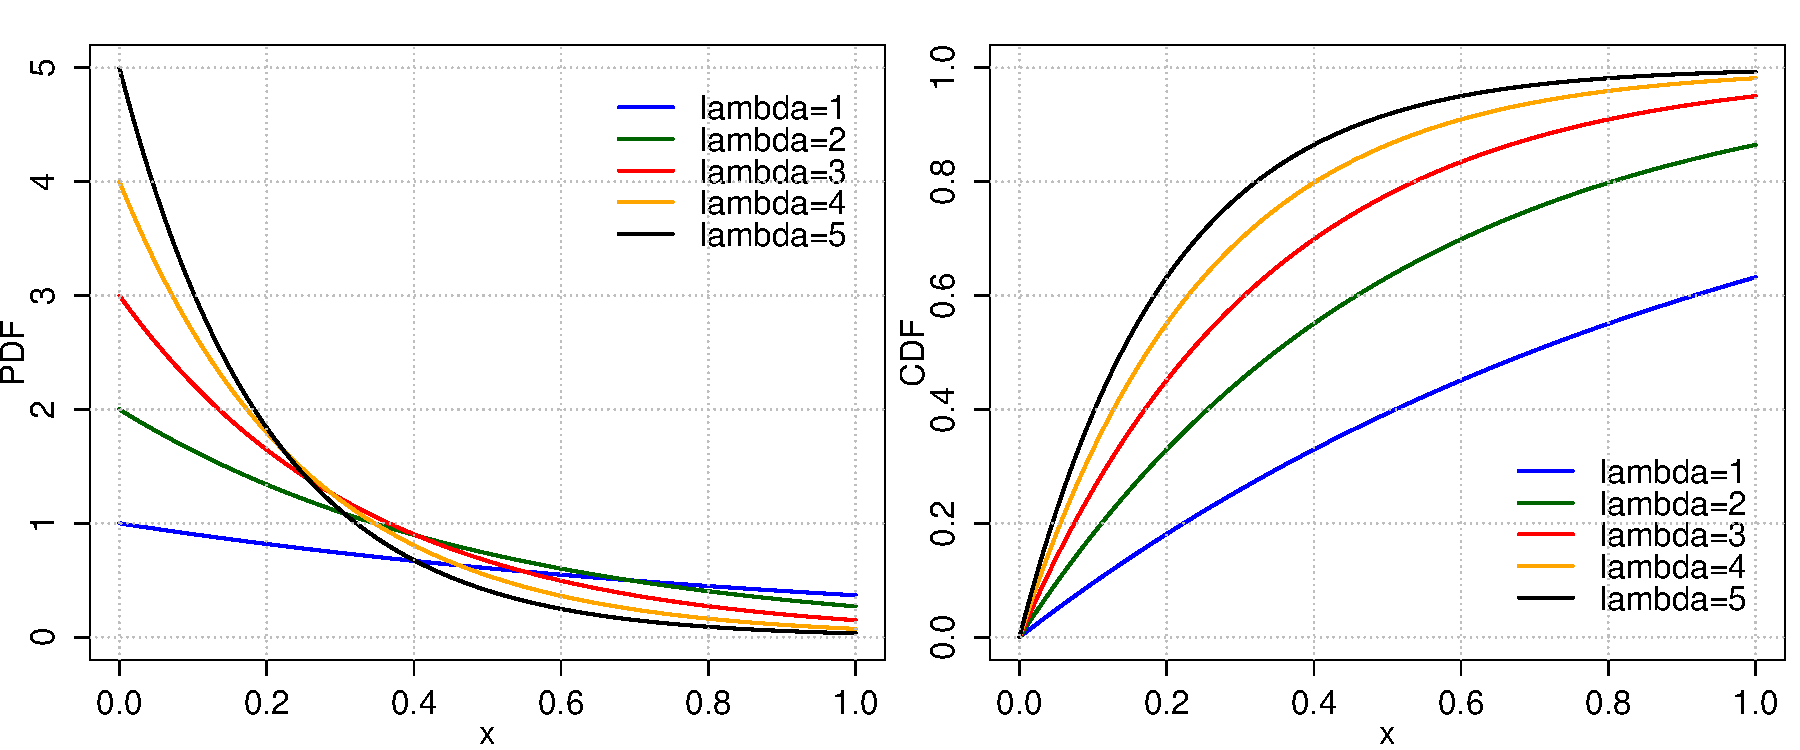
\includegraphics[width=140mm]{pics/Exponential.pdf}
 \caption{Exponential distribution plotted using the provided R code.}
 \label{fig:Exponential}
\end{figure}

\subsubsection*{Parameter: rate}

\noindent\begin{tabular}{p{2cm}cl}
\textbf{name} & & rate or inverse scale \\
\textbf{type} & & scalar \\
\textbf{symbol} & & $\lambda$  \\
\textbf{definition} & & $\lambda > 0$
\end{tabular}
\subsubsection*{Functions}

\smallskip \noindent \hspace{.2cm} \textbf{PDF} 
\begin{equation*}\lambda e^{-\lambda x}\end{equation*}
\smallskip \noindent \hspace{.2cm} \textbf{PDF in R}  
\begin{verbatim}lambda*exp(-lambda*x)\end{verbatim}
\smallskip \noindent \hspace{.2cm} \textbf{CDF} 
\begin{equation*}1 - e^{-\lambda x}\end{equation*}
\smallskip \noindent \hspace{.2cm} \textbf{CDF in R} 
\begin{verbatim}1 - exp(-lambda*x)\end{verbatim}
\smallskip
\subsubsection*{Characteristics}
\smallskip \noindent \hspace{.2cm} \textbf{Mean} 
\begin{equation*}\lambda^{-1}\end{equation*}
\smallskip \noindent \hspace{.2cm} \textbf{Median} 
\begin{equation*}\lambda^{-1} ln(2)\end{equation*}
\smallskip \noindent \hspace{.2cm} \textbf{Mode} 
\begin{equation*}0\end{equation*}
\smallskip \noindent \hspace{.2cm} \textbf{Variance} 
\begin{equation*}\lambda^{-2}\end{equation*}
\smallskip
\section*{F1} 

  \bigskip 

\begin{tabular}{p{2cm}cl}
\textbf{name} & & F (ID: 0000113)\\ 
 
\textbf{type} & & continuous \\ 

\textbf{variate} & & $x$, scalar \\ 

\textbf{support} & & $x \in [0,+\infty)$
\end{tabular}

\begin{figure}[ht!]
\centering
  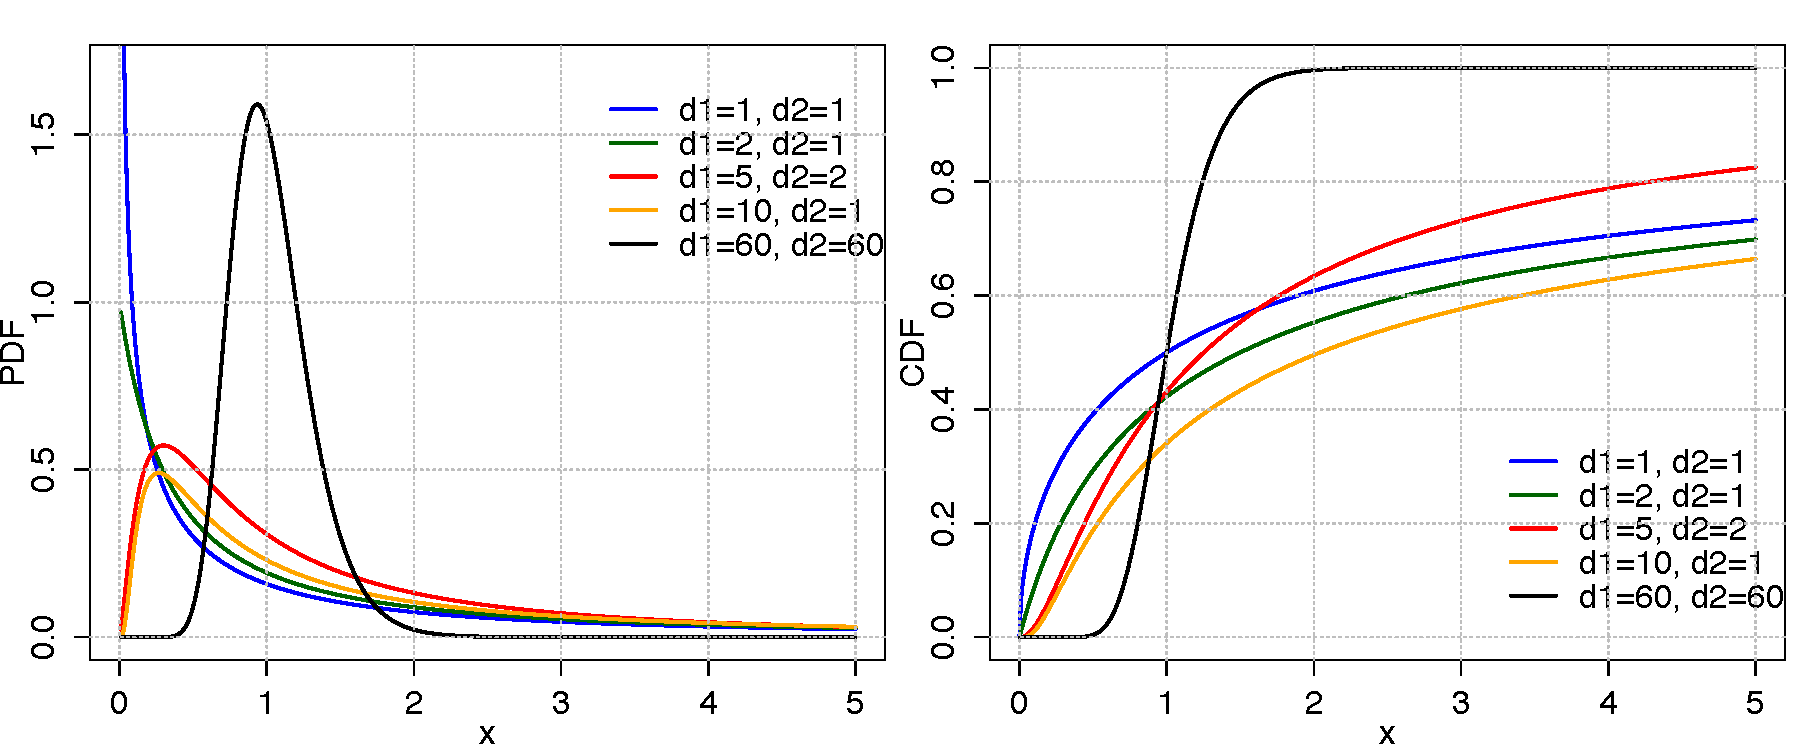
\includegraphics[width=140mm]{pics/F.pdf}
 \caption{F distribution plotted using the provided R code.}
 \label{fig:F}
\end{figure}

\subsubsection*{Parameter: numerator}

\noindent\begin{tabular}{p{2cm}cl}
\textbf{name} & & degree of freedom \\
\textbf{type} & & scalar \\
\textbf{symbol} & & $d_1$  \\
\textbf{definition} & & $d_1 > 0$
\end{tabular}
\subsubsection*{Parameter: denominator}

\noindent\begin{tabular}{p{2cm}cl}
\textbf{name} & & degree of freedom \\
\textbf{type} & & scalar \\
\textbf{symbol} & & $d_2$  \\
\textbf{definition} & & $d_2 > 0$
\end{tabular}
\subsubsection*{Functions}

\smallskip \noindent \hspace{.2cm} \textbf{PDF} 
\begin{equation*}\frac{\sqrt{\frac{(d_1 x)^{d_1}d_2^{d_2}}
{(d_1 x+d_2)^{d_1+d_2}}}}
{x B\left(\frac{d_1}{2},\frac{d_2}{2}\right)}\end{equation*}
\smallskip \noindent \hspace{.2cm} \textbf{PDF in R}  
\begin{verbatim}sqrt((d1*x)^d1*d2^(d2) / (d1*x+d2)^(d1+d2) ) / (x*beta(d1/2,d2/2))\end{verbatim}
\smallskip \noindent \hspace{.2cm} \textbf{CDF} 
\begin{equation*}I_{\frac{d_1 x}{d_1 x + d_2}} \left(\tfrac{d_1}{2}, \tfrac{d_2}{2} \right)\end{equation*}
\smallskip \noindent \hspace{.2cm} \textbf{CDF in R} 
\begin{verbatim}Rbeta(d1*x / (d1*x + d2), d1/2, d2/2)\end{verbatim}
\smallskip
\subsubsection*{Characteristics}
\smallskip \noindent \hspace{.2cm} \textbf{Mean} 
\begin{equation*}\frac{d_2}{d_2-2} \quad \text{for} \quad d_2 > 0\end{equation*}
\smallskip \noindent \hspace{.2cm} \textbf{Mode} 
\begin{equation*}\frac{d_1-2}{d_1}\;\frac{d_2}{d_2+2} \quad \text{for} \quad d_1 > 0\end{equation*}
\smallskip \noindent \hspace{.2cm} \textbf{Variance} 
\begin{equation*}\frac{2\,d_2^2\,(d_1+d_2-2)}{d_1 (d_2-2)^2 (d_2-4)} \quad \text{for} \quad d_2 > 4\end{equation*}
\smallskip
\section*{Gamma1} 

  \bigskip 

\begin{tabular}{p{2cm}cl}
\textbf{name} & & Gamma (ID: 0000123)\\ 
 
\textbf{type} & & continuous \\ 

\textbf{variate} & & $x$, scalar \\ 

\textbf{support} & & $x \in (0,+\infty)$
\end{tabular}

\begin{figure}[ht!]
\centering
  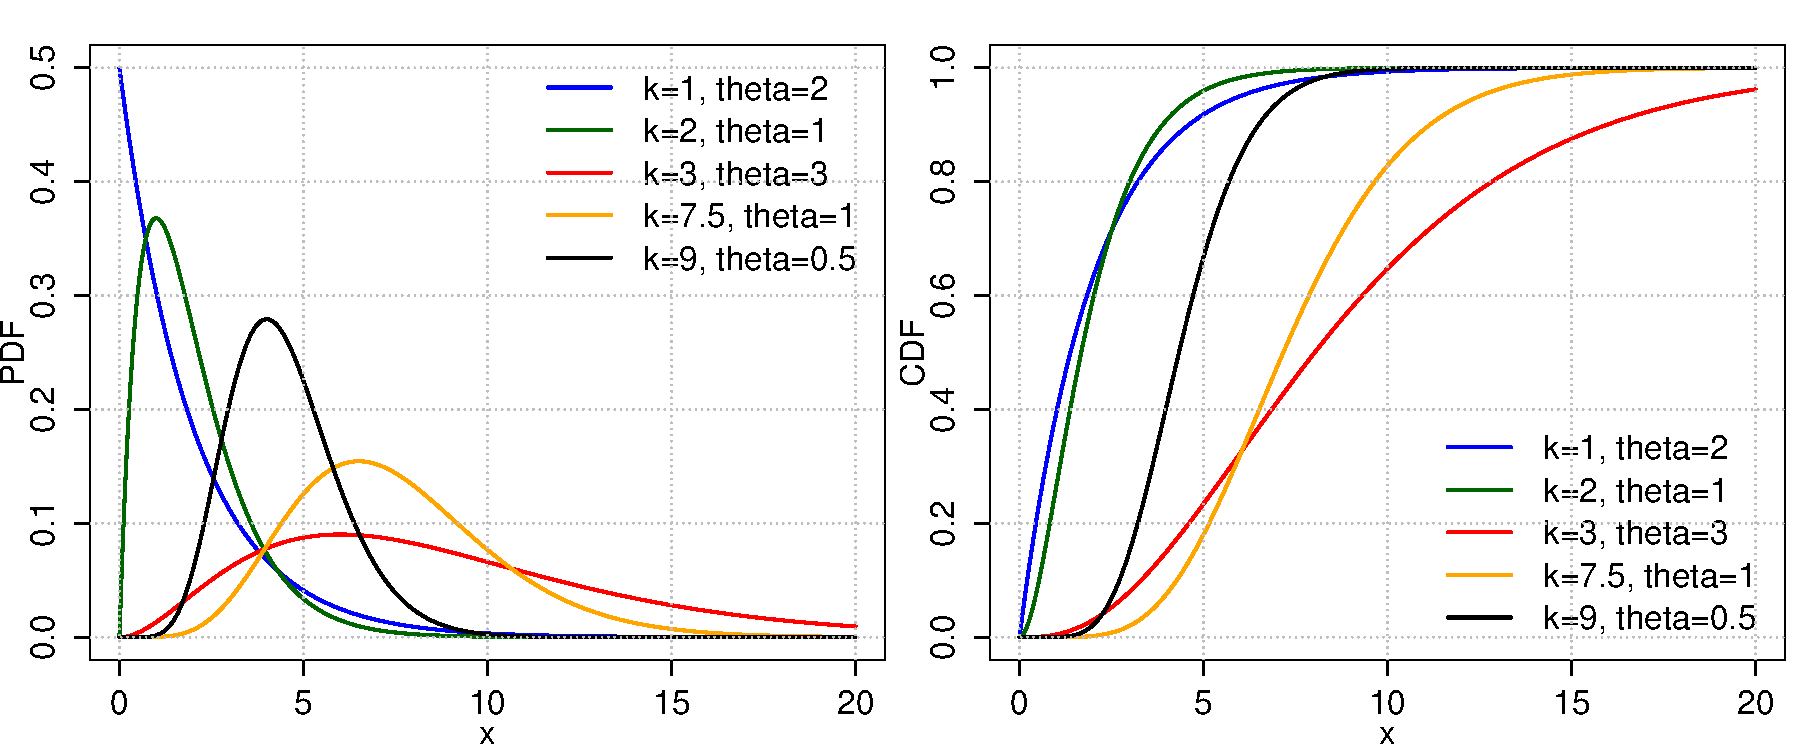
\includegraphics[width=140mm]{pics/Gamma.pdf}
 \caption{Gamma distribution plotted using the provided R code.}
 \label{fig:Gamma}
\end{figure}

\subsubsection*{Parameter: shape}

\noindent\begin{tabular}{p{2cm}cl}
\textbf{name} & & shape \\
\textbf{type} & & scalar \\
\textbf{symbol} & & $k$  \\
\textbf{definition} & & $k > 0$
\end{tabular}
\subsubsection*{Parameter: scale}

\noindent\begin{tabular}{p{2cm}cl}
\textbf{name} & & scale \\
\textbf{type} & & scalar \\
\textbf{symbol} & & $\theta$  \\
\textbf{definition} & & $\theta > 0$
\end{tabular}
\subsubsection*{Functions}

\smallskip \noindent \hspace{.2cm} \textbf{PDF} 
\begin{equation*}\frac{1}{\Gamma(k) \theta^k} x^{k \,-\, 1} e^{-\frac{x}{\theta}}\end{equation*}
\smallskip \noindent \hspace{.2cm} \textbf{PDF in R}  
\begin{verbatim}1 / (gamma(k) * theta^k) * x^(k-1) * exp(-x/theta)\end{verbatim}
\smallskip \noindent \hspace{.2cm} \textbf{CDF} 
\begin{equation*}\frac{1}{\Gamma(k)} \gamma\left(k,\, \frac{x}{\theta}\right)\end{equation*}
\smallskip \noindent \hspace{.2cm} \textbf{CDF in R} 
\begin{verbatim}1/gamma(k) * Igamma(k,x/theta)\end{verbatim}
\smallskip
\subsubsection*{Characteristics}
\smallskip \noindent \hspace{.2cm} \textbf{Mean} 
\begin{equation*}k \theta\end{equation*}
\smallskip \noindent \hspace{.2cm} \textbf{Median} 
\begin{equation*}\text{No simple closed form}\end{equation*}
\smallskip \noindent \hspace{.2cm} \textbf{Mode} 
\begin{equation*}(k \,-\, 1)\theta \text{ for } k \;{\geq}\; 1\end{equation*}
\smallskip \noindent \hspace{.2cm} \textbf{Variance} 
\begin{equation*}k \theta^2\end{equation*}
\smallskip
\section*{GeneralizedGamma1} 

  \bigskip 

\begin{tabular}{p{2cm}cl}
\textbf{name} & & Generalized Gamma 1 (ID: 0000142)\\ 
 
\textbf{type} & & continuous \\ 

\textbf{variate} & & $x$, scalar \\ 

\textbf{support} & & $x \in (0,+\infty)$
\end{tabular}

\begin{figure}[ht!]
\centering
  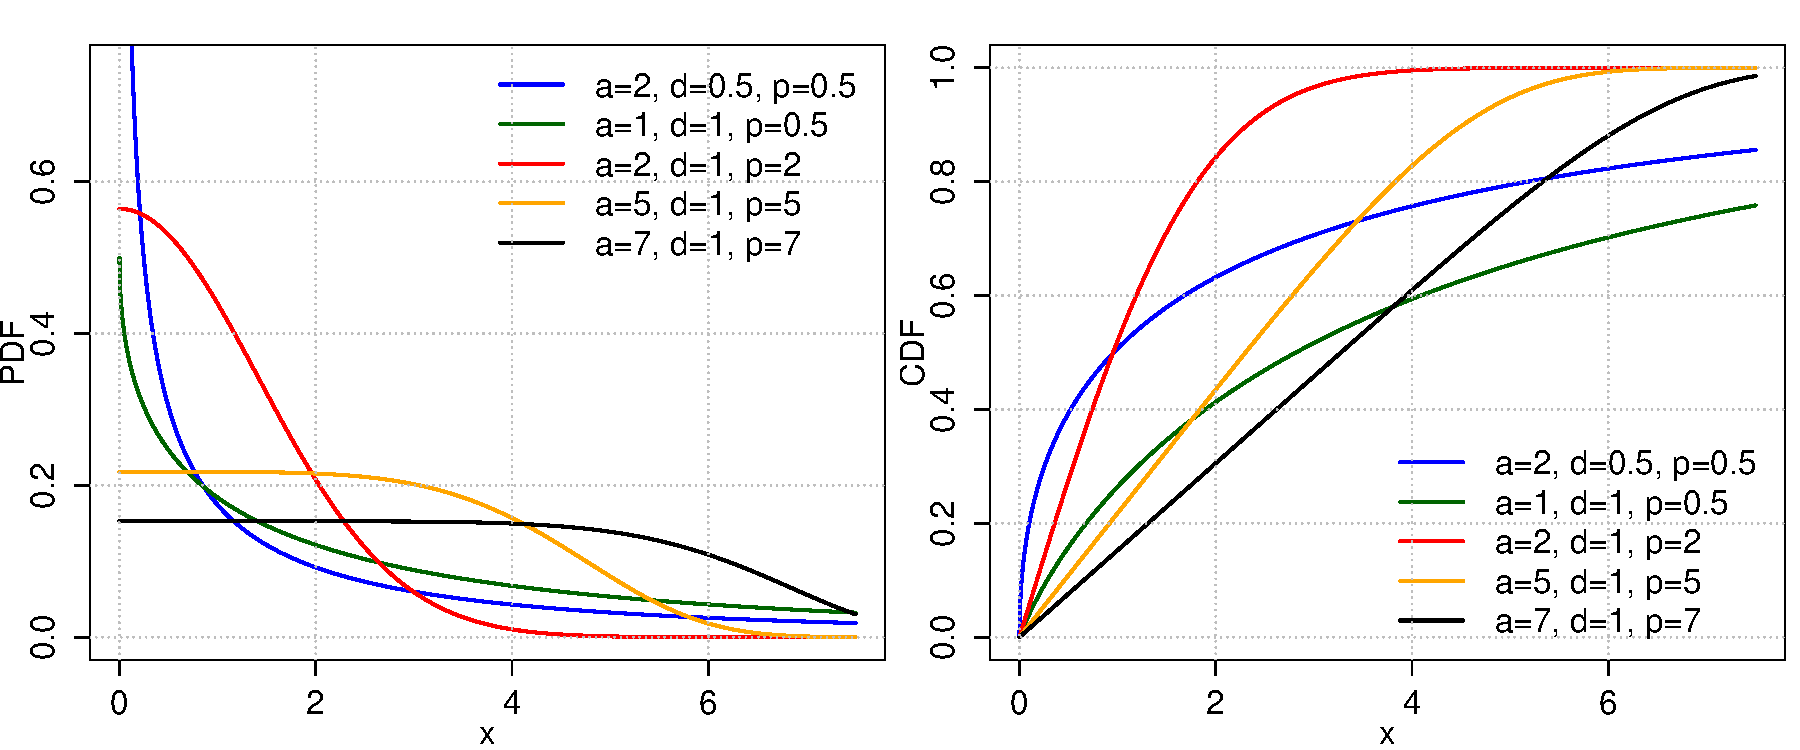
\includegraphics[width=140mm]{pics/GeneralizedGamma1.pdf}
 \caption{GeneralizedGamma1 distribution plotted using the provided R code.}
 \label{fig:GeneralizedGamma1}
\end{figure}

\subsubsection*{Parameter: scale}

\noindent\begin{tabular}{p{2cm}cl}
\textbf{name} & & scale \\
\textbf{type} & & scalar \\
\textbf{symbol} & & $a$  \\
\textbf{definition} & & $a > 0$
\end{tabular}
\subsubsection*{Parameter: shape1}

\noindent\begin{tabular}{p{2cm}cl}
\textbf{name} & & shape \\
\textbf{type} & & scalar \\
\textbf{symbol} & & $d$  \\
\textbf{definition} & & $d > 0$
\end{tabular}
\subsubsection*{Parameter: shape2}

\noindent\begin{tabular}{p{2cm}cl}
\textbf{name} & & shape \\
\textbf{type} & & - \\
\textbf{symbol} & & $p$  \\
\textbf{definition} & & $p > 0$
\end{tabular}
\subsubsection*{Functions}

\smallskip \noindent \hspace{.2cm} \textbf{PDF} 
\begin{equation*}\frac{p/a^d}{\Gamma(d/p)} x^{d-1}e^{-(x/a)^p}\end{equation*}
\smallskip \noindent \hspace{.2cm} \textbf{PDF in R}  
\begin{verbatim}p/a^d/gamma(d/p) * x^(d-1) * exp(-(x/a)^p)\end{verbatim}
\smallskip \noindent \hspace{.2cm} \textbf{CDF} 
\begin{equation*}\frac{\gamma(d/p, (x/a)^p)}{\Gamma(d/p)}\end{equation*}
\smallskip \noindent \hspace{.2cm} \textbf{CDF in R} 
\begin{verbatim}Igamma(d/p, (x/a)^p, lower=T) / gamma(d/p)\end{verbatim}
\smallskip
\subsubsection*{Characteristics}
\smallskip \noindent \hspace{.2cm} \textbf{Mean} 
\begin{equation*}a \frac{\Gamma((d+1)/p)}{\Gamma(d/p)}\end{equation*}
\smallskip \noindent \hspace{.2cm} \textbf{Mode} 
\begin{equation*}a \left(\frac{d-1}{p}\right)^{\frac{1}{p}}, \text{ for } d>1\end{equation*}
\smallskip \noindent \hspace{.2cm} \textbf{Variance} 
\begin{equation*}a^2\left(\frac{\Gamma((d+2)/p)}{\Gamma(d/p)} - \left(\frac{\Gamma((d+1)/p)}{\Gamma(d/p)}\right)^2\right)\end{equation*}
\smallskip
\section*{GeneralizedGamma2} 

  \bigskip 

\begin{tabular}{p{2cm}cl}
\textbf{name} & & Generalized Gamma 2 (ID: 0000153)\\ 
 
\textbf{type} & & continuous \\ 

\textbf{variate} & & $x$, scalar \\ 

\textbf{support} & & $0 < a < x$
\end{tabular}

\begin{figure}[ht!]
\centering
  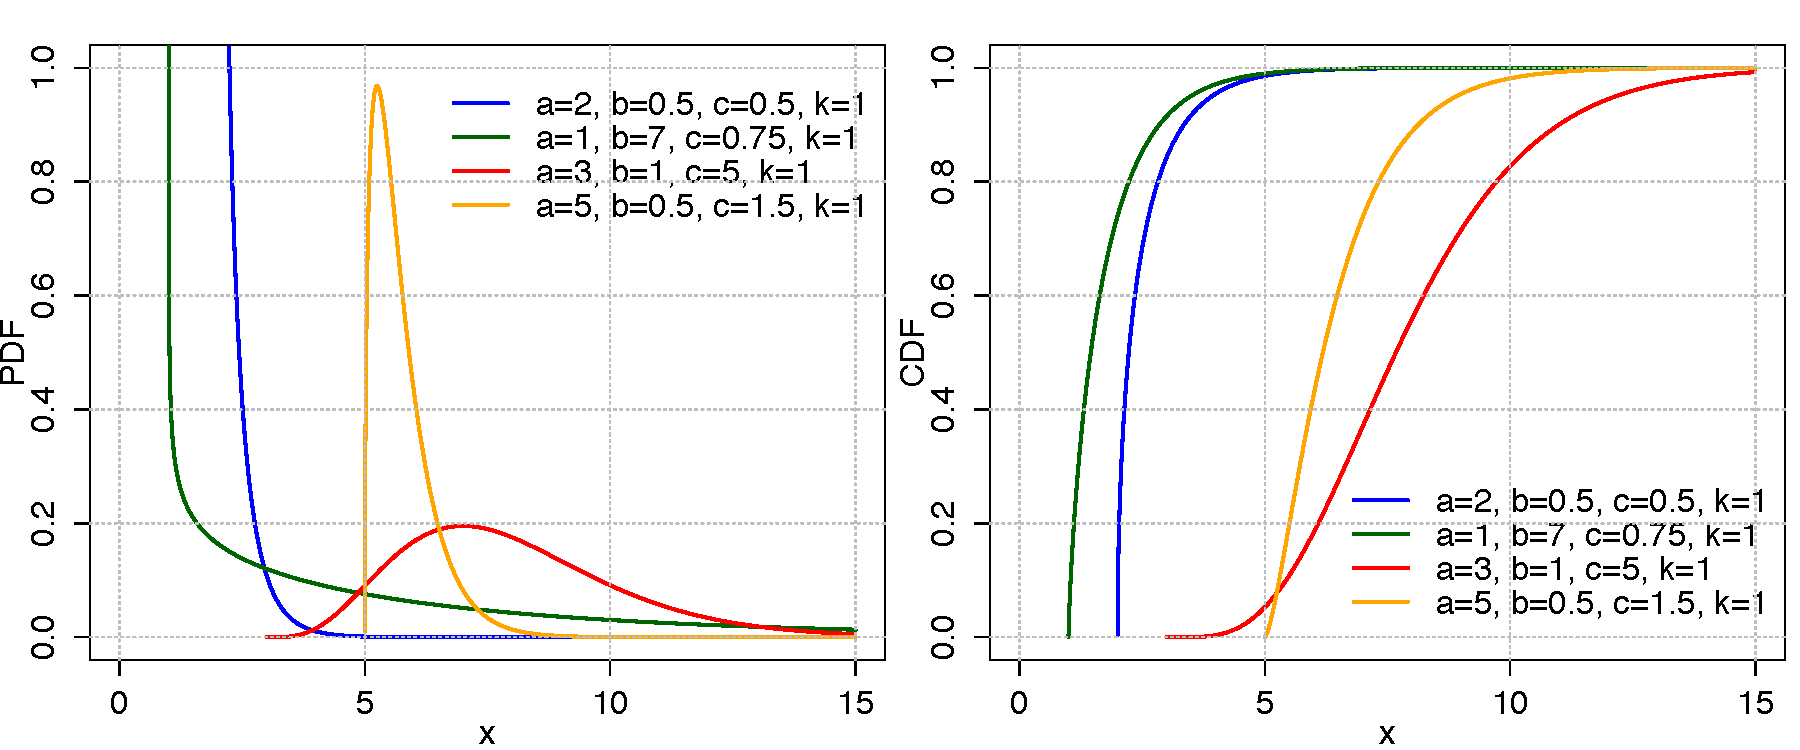
\includegraphics[width=140mm]{pics/GeneralizedGamma2.pdf}
 \caption{GeneralizedGamma2 distribution plotted using the provided R code.}
 \label{fig:GeneralizedGamma2}
\end{figure}

\subsubsection*{Parameter: location}

\noindent\begin{tabular}{p{2cm}cl}
\textbf{name} & & location \\
\textbf{type} & & scalar \\
\textbf{symbol} & & $a$  \\
\textbf{definition} & & $a > 0$
\end{tabular}
\subsubsection*{Parameter: scale}

\noindent\begin{tabular}{p{2cm}cl}
\textbf{name} & & scale \\
\textbf{type} & & scalar \\
\textbf{symbol} & & $b$  \\
\textbf{definition} & & $b > 0$
\end{tabular}
\subsubsection*{Parameter: shape1}

\noindent\begin{tabular}{p{2cm}cl}
\textbf{name} & & shape1 \\
\textbf{type} & & scalar \\
\textbf{symbol} & & $c$  \\
\textbf{definition} & & $c > 0$
\end{tabular}
\subsubsection*{Parameter: shape2}

\noindent\begin{tabular}{p{2cm}cl}
\textbf{name} & & shape2 \\
\textbf{type} & & scalar \\
\textbf{symbol} & & $k$  \\
\textbf{definition} & & $k > 0$
\end{tabular}
\subsubsection*{Functions}

\smallskip \noindent \hspace{.2cm} \textbf{PDF} 
\begin{equation*}\frac{k (x-a)^{kc-1}}{b^{kc}\Gamma(c)}\exp\Big[-\Big(\frac{x-a}{b}\Big)^k\Big]\end{equation*}
\smallskip \noindent \hspace{.2cm} \textbf{PDF in R}  
\begin{verbatim}(k*(x-a)^(k*c-1)) / (b^(k*c)*gamma(c)) * exp( -((x-a)/b)^k )\end{verbatim}
\smallskip \noindent \hspace{.2cm} \textbf{CDF} 
\begin{equation*}\frac{\gamma(c,(\frac{x-a}{b})^k)}{\Gamma(c)}\end{equation*}
\smallskip \noindent \hspace{.2cm} \textbf{CDF in R} 
\begin{verbatim}Igamma(c, ((x-a)/b)^k, lower=T) / gamma(c)\end{verbatim}
\smallskip
\subsubsection*{Characteristics}
\smallskip \noindent \hspace{.2cm} \textbf{Mean} 
\begin{equation*}a + b\Gamma(c+1/k)/\Gamma(c)\end{equation*}
\smallskip \noindent \hspace{.2cm} \textbf{Mode} 
\begin{equation*}a+b(c-1/k)^{1/k}, c>1/k\end{equation*}
\smallskip \noindent \hspace{.2cm} \textbf{Variance} 
\begin{equation*}b^2\{\Gamma(c+2/k)/\Gamma(c)-[\Gamma(c+1/k)/\Gamma(c)]^2\}\end{equation*}
\smallskip
\section*{GeneralizedPoisson1} 

  \bigskip 

\begin{tabular}{p{2cm}cl}
\textbf{name} & & Generalized Poisson (ID: 0000165)\\ 
 
\textbf{type} & & discrete \\ 

\textbf{variate} & & $k
$, scalar \\ 

\textbf{support} & & $k \in \{0,1,2,3,\dots\}$
\end{tabular}

\begin{figure}[ht!]
\centering
  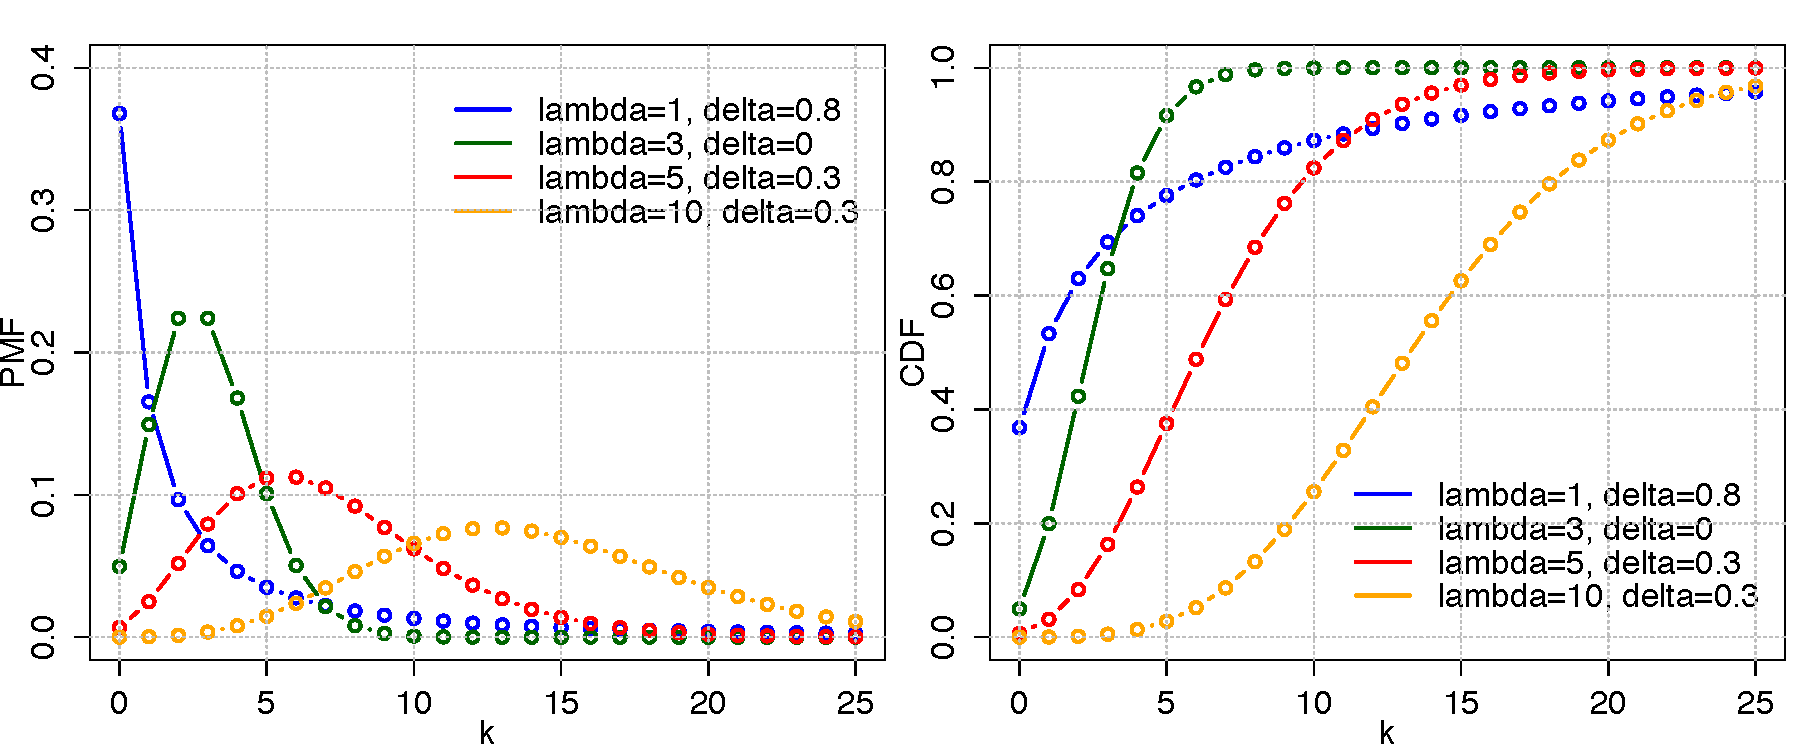
\includegraphics[width=140mm]{pics/GeneralizedPoisson.pdf}
 \caption{GeneralizedPoisson distribution plotted using the provided R code.}
 \label{fig:GeneralizedPoisson}
\end{figure}

\subsubsection*{Parameter: rate}

\noindent\begin{tabular}{p{2cm}cl}
\textbf{name} & & Poisson intensity \\
\textbf{type} & & scalar \\
\textbf{symbol} & & $\lambda$  \\
\textbf{definition} & & $\lambda \in R, \lambda > 0$
\end{tabular}
\subsubsection*{Parameter: dispersion}

\noindent\begin{tabular}{p{2cm}cl}
\textbf{name} & & dispersion \\
\textbf{type} & & scalar \\
\textbf{symbol} & & $\delta$  \\
\textbf{definition} & & $\max(-1,-\lambda/4) < \delta < 1$
\end{tabular}
\subsubsection*{Functions}

\smallskip \noindent \hspace{.2cm} \textbf{PMF} 
\begin{equation*}\frac{\lambda (\lambda+k\delta)^{k-1}\times e^{-\lambda - k \delta}}{k!}\end{equation*}
\smallskip \noindent \hspace{.2cm} \textbf{PMF in R}  
\begin{verbatim}(lambda*(lambda+k*delta)^(k-1) * exp(-lambda-k*delta)) / factorial(k)\end{verbatim}
\smallskip \noindent \hspace{.2cm} \textbf{CDF} 
\begin{equation*}\Sigma_{i=1}^x f(i), x \in \{0,1,2,...\}
\text { with f the PMF}\end{equation*}
\smallskip \noindent \hspace{.2cm} \textbf{CDF in R}  
\begin{verbatim}
cumsum(PMF)
\end{verbatim}
\smallskip
\subsubsection*{Characteristics}
\smallskip \noindent \hspace{.2cm} \textbf{Mean} 
\begin{equation*}\frac{\lambda}{1 -\delta}\end{equation*}
\smallskip \noindent \hspace{.2cm} \textbf{Variance} 
\begin{equation*}\frac{\lambda}{(1 -\delta)^3}\end{equation*}
\smallskip
\section*{Geometric1} 

  \bigskip 

\begin{tabular}{p{2cm}cl}
\textbf{name} & & Geometric (ID: 0000133)\\ 
 
\textbf{type} & & discrete \\ 

\textbf{variate} & & $k
$, scalar \\ 

\textbf{support} & & $k \in \{0,1,2,3,\dots\}$
\end{tabular}

\begin{figure}[ht!]
\centering
  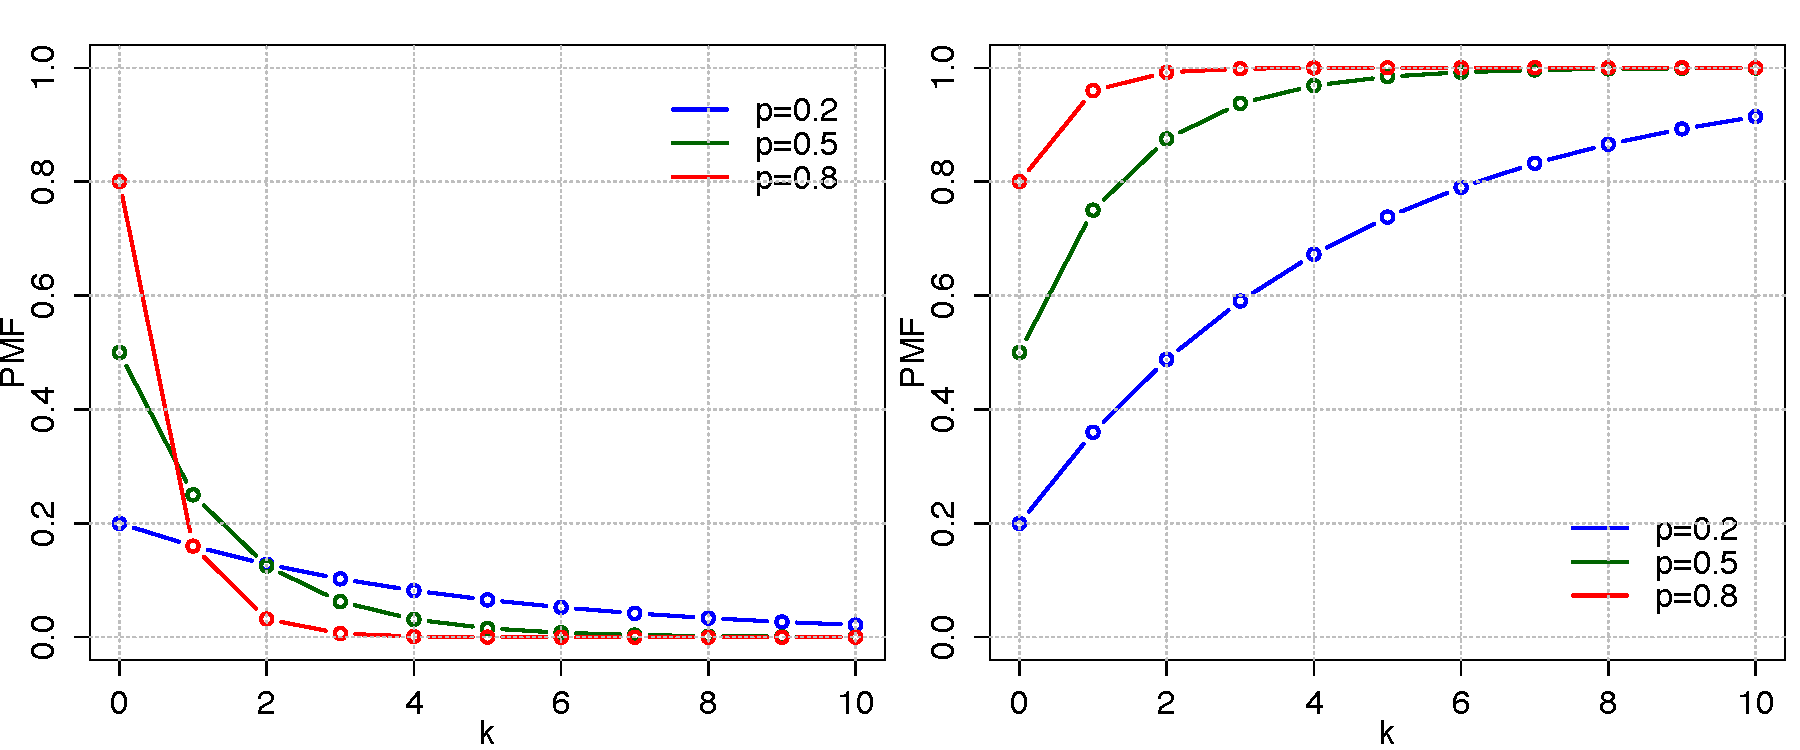
\includegraphics[width=140mm]{pics/Geometric.pdf}
 \caption{Geometric distribution plotted using the provided R code.}
 \label{fig:Geometric}
\end{figure}

\subsubsection*{Parameter: probability}

\noindent\begin{tabular}{p{2cm}cl}
\textbf{name} & & success probability \\
\textbf{type} & & scalar \\
\textbf{symbol} & & $p$  \\
\textbf{definition} & & $0< p \leq 1$
\end{tabular}
\subsubsection*{Functions}

\smallskip \noindent \hspace{.2cm} \textbf{PMF} 
\begin{equation*}(1 - p)^k\,p\end{equation*}
\smallskip \noindent \hspace{.2cm} \textbf{PMF in R}  
\begin{verbatim}p*(1-p)^k\end{verbatim}
\smallskip \noindent \hspace{.2cm} \textbf{CDF} 
\begin{equation*}1-(1 - p)^{k+1}\end{equation*}
\smallskip \noindent \hspace{.2cm} \textbf{CDF in R} 
\begin{verbatim}1-(1 - p)^(k+1)\end{verbatim}
\smallskip
\subsubsection*{Characteristics}
\smallskip \noindent \hspace{.2cm} \textbf{Mean} 
\begin{equation*}\frac{1-p}{p}\end{equation*}
\smallskip \noindent \hspace{.2cm} \textbf{Median} 
\begin{equation*}\left\lceil \frac{-1}{\log_2(1-p)}-1 \right\rceil \text{ (not unique if } -1/\log_2(1-p)-1 \text{ is an integer)}\end{equation*}
\smallskip \noindent \hspace{.2cm} \textbf{Mode} 
\begin{equation*}0\end{equation*}
\smallskip \noindent \hspace{.2cm} \textbf{Variance} 
\begin{equation*}\frac{1-p}{p^2}\end{equation*}
\smallskip
\section*{Gompertz1} 

  \bigskip 

\begin{tabular}{p{2cm}cl}
\textbf{name} & & Gompertz (ID: 0000175)\\ 
 
\textbf{type} & & continuous \\ 

\textbf{variate} & & $x$, scalar \\ 

\textbf{support} & & $x \in (-\infty,+\infty)$
\end{tabular}

\begin{figure}[ht!]
\centering
  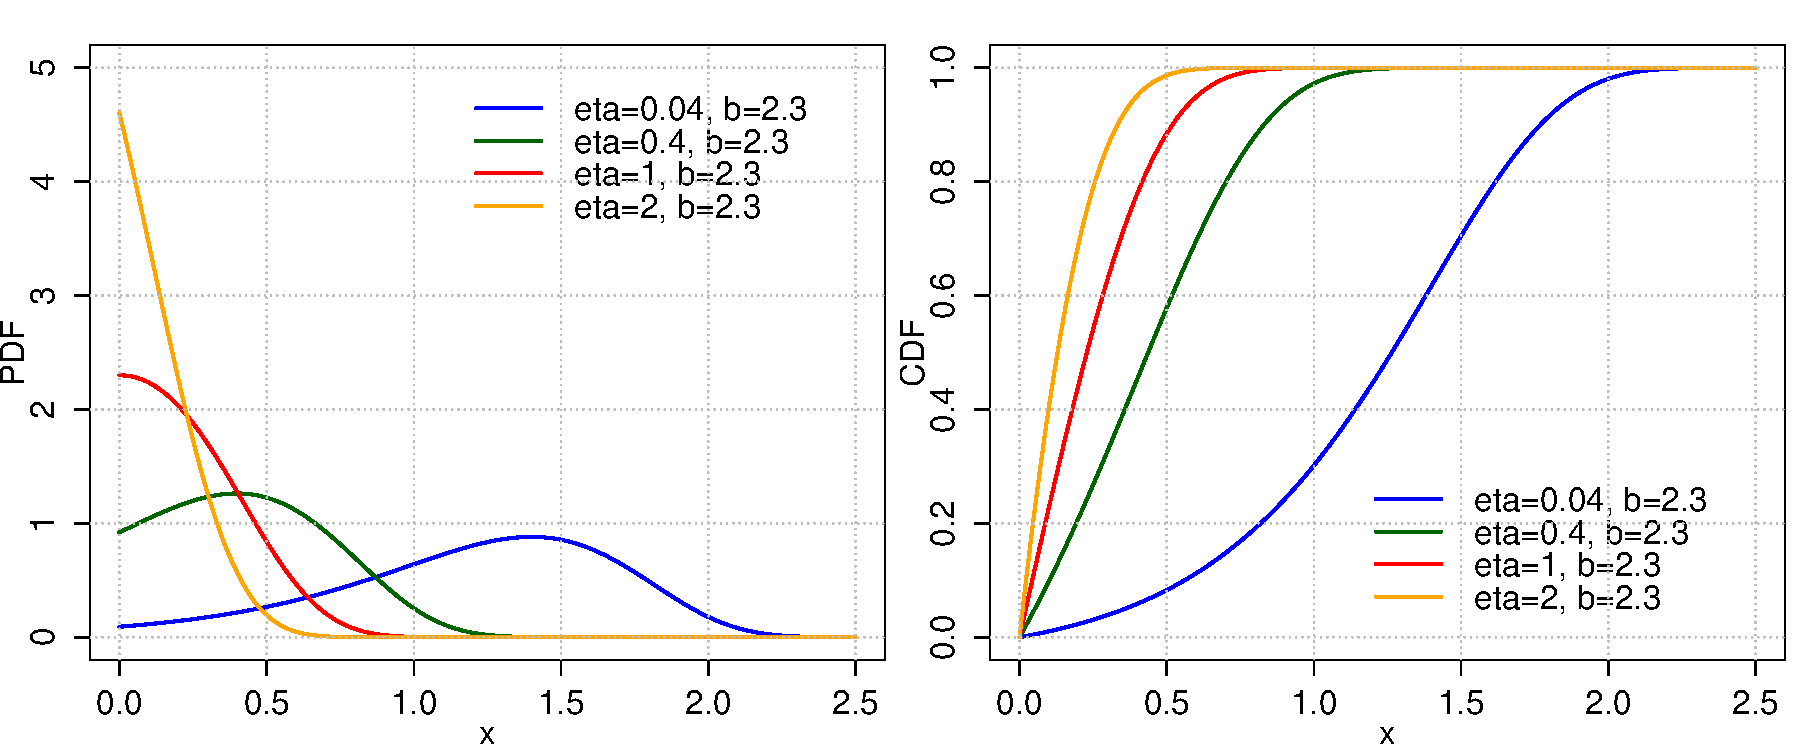
\includegraphics[width=140mm]{pics/Gompertz.pdf}
 \caption{Gompertz distribution plotted using the provided R code.}
 \label{fig:Gompertz}
\end{figure}

\subsubsection*{Parameter: shape}

\noindent\begin{tabular}{p{2cm}cl}
\textbf{name} & & shape \\
\textbf{type} & & scalar \\
\textbf{symbol} & & $\eta$  \\
\textbf{definition} & & $\eta > 0$
\end{tabular}
\subsubsection*{Parameter: scale}

\noindent\begin{tabular}{p{2cm}cl}
\textbf{name} & & scale \\
\textbf{type} & & scalar \\
\textbf{symbol} & & $b$  \\
\textbf{definition} & & $b > 0$
\end{tabular}
\subsubsection*{Functions}

\smallskip \noindent \hspace{.2cm} \textbf{PDF} 
\begin{equation*}b\eta e^{bx}e^{\eta}\exp\left(-\eta e^{bx} \right)\end{equation*}
\smallskip \noindent \hspace{.2cm} \textbf{PDF in R}  
\begin{verbatim}b*eta*exp(b*x)*exp(eta)*exp(-eta*exp(b*x))\end{verbatim}
\smallskip \noindent \hspace{.2cm} \textbf{CDF} 
\begin{equation*}1-\exp\left(-\eta\left(e^{bx}-1 \right)\right)\end{equation*}
\smallskip \noindent \hspace{.2cm} \textbf{CDF in R} 
\begin{verbatim}1-exp(-eta*(exp(b*x)-1))\end{verbatim}
\smallskip
\subsubsection*{Characteristics}
\smallskip \noindent \hspace{.2cm} \textbf{Median} 
\begin{equation*}\left(1/b\right)\log\left[\left(-1/\eta\right) \log\left(1/2\right)+1\right]\end{equation*}
\smallskip
\section*{Gumbel1} 

  \bigskip 

\begin{tabular}{p{2cm}cl}
\textbf{name} & & Gumbel (ID: 0000187)\\ 
 
\textbf{type} & & continuous \\ 

\textbf{variate} & & $x$, scalar \\ 

\textbf{support} & & $x \in (-\infty,+\infty)$
\end{tabular}

\begin{figure}[ht!]
\centering
  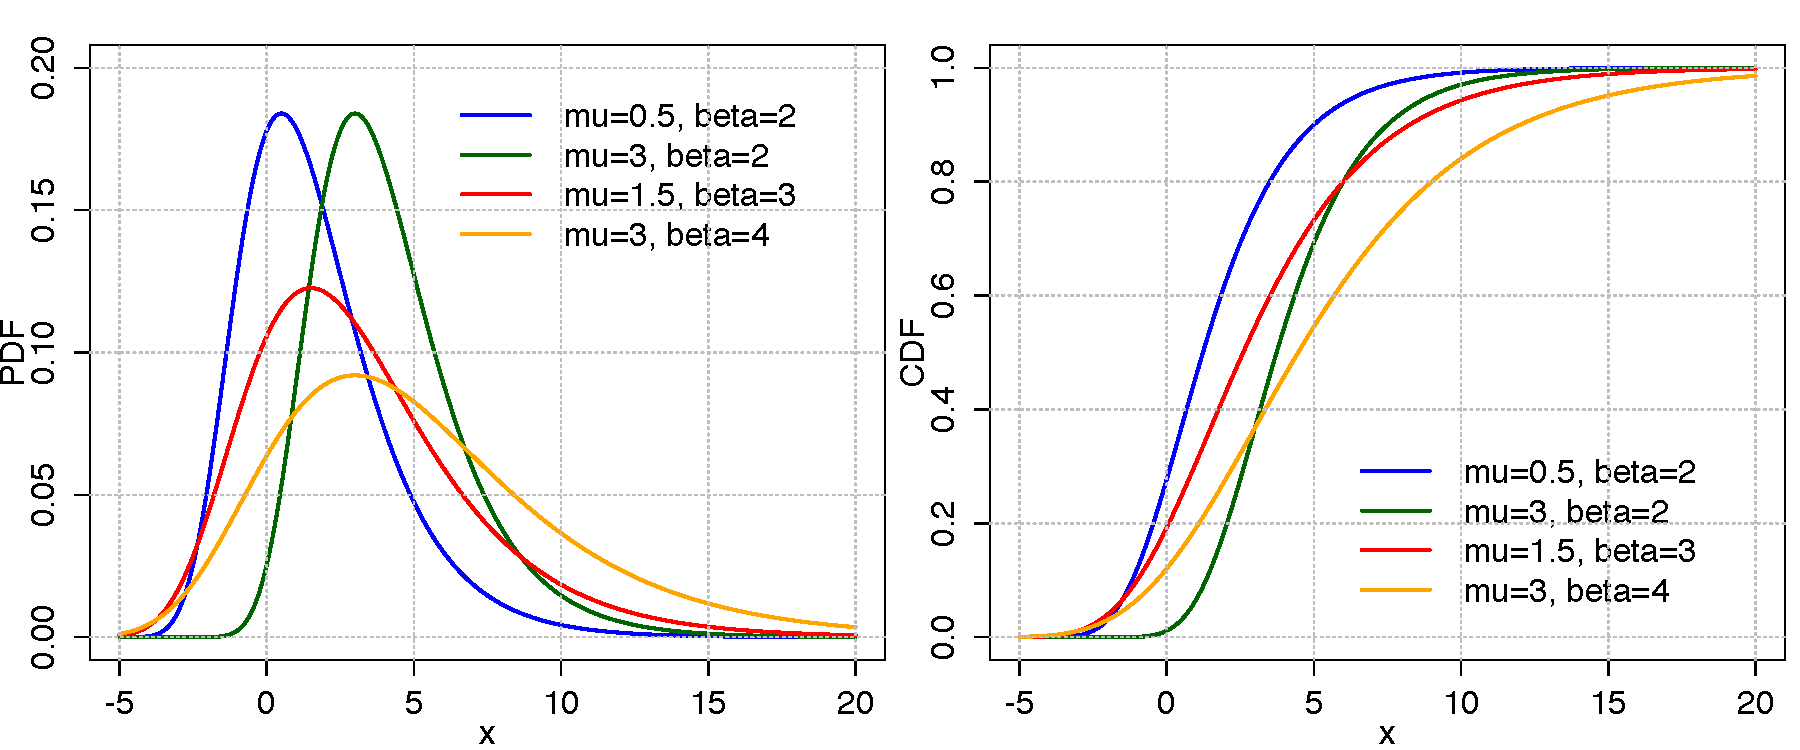
\includegraphics[width=140mm]{pics/Gumbel.pdf}
 \caption{Gumbel distribution plotted using the provided R code.}
 \label{fig:Gumbel}
\end{figure}

\subsubsection*{Parameter: location}

\noindent\begin{tabular}{p{2cm}cl}
\textbf{name} & & location \\
\textbf{type} & & scalar \\
\textbf{symbol} & & $\mu$  \\
\textbf{definition} & & $\mu \in  R$
\end{tabular}
\subsubsection*{Parameter: scale}

\noindent\begin{tabular}{p{2cm}cl}
\textbf{name} & & scale \\
\textbf{type} & & scalar \\
\textbf{symbol} & & $\beta$  \\
\textbf{definition} & & $\beta>0, \beta \in  R$
\end{tabular}
\subsubsection*{Functions}

\smallskip \noindent \hspace{.2cm} \textbf{PDF} 
\begin{equation*}\frac{e^{-e^{-\frac{x-\mu}{\beta}}} e^{-\frac{x-\mu}{\beta}}}{\beta}\end{equation*}
\smallskip \noindent \hspace{.2cm} \textbf{PDF in R}  
\begin{verbatim}(exp(-exp(-(x-mu)/beta)) * exp(-(x-mu)/beta))/beta\end{verbatim}
\smallskip \noindent \hspace{.2cm} \textbf{CDF} 
\begin{equation*}e^{-e^{-(x-\mu)/\beta}}\end{equation*}
\smallskip \noindent \hspace{.2cm} \textbf{CDF in R} 
\begin{verbatim}exp(-exp(-(x-mu)/beta))\end{verbatim}
\smallskip
\subsubsection*{Characteristics}
\smallskip \noindent \hspace{.2cm} \textbf{Mean} 
\begin{equation*}\mu + \beta\,\gamma; \text{ with } \gamma \text{ is Euler constant }\end{equation*}
\smallskip \noindent \hspace{.2cm} \textbf{Median} 
\begin{equation*}\mu - \beta\,\ln(\ln(2))\end{equation*}
\smallskip \noindent \hspace{.2cm} \textbf{Mode} 
\begin{equation*}\mu\end{equation*}
\smallskip \noindent \hspace{.2cm} \textbf{Variance} 
\begin{equation*}\frac{\pi^2}{6} \beta^2\end{equation*}
\smallskip
\section*{Hypergeometric1} 

  \bigskip 

\begin{tabular}{p{2cm}cl}
\textbf{name} & & Hypergeometric (ID: 0000197)\\ 
 
\textbf{type} & & discrete \\ 

\textbf{variate} & & $k$, scalar \\ 

\textbf{support} & & $k\, \in\, \left\{\max{(0,\, n+K-N)},\, \dots,\, \min{(n,\, K )}\right\}$
\end{tabular}

\begin{figure}[ht!]
\centering
  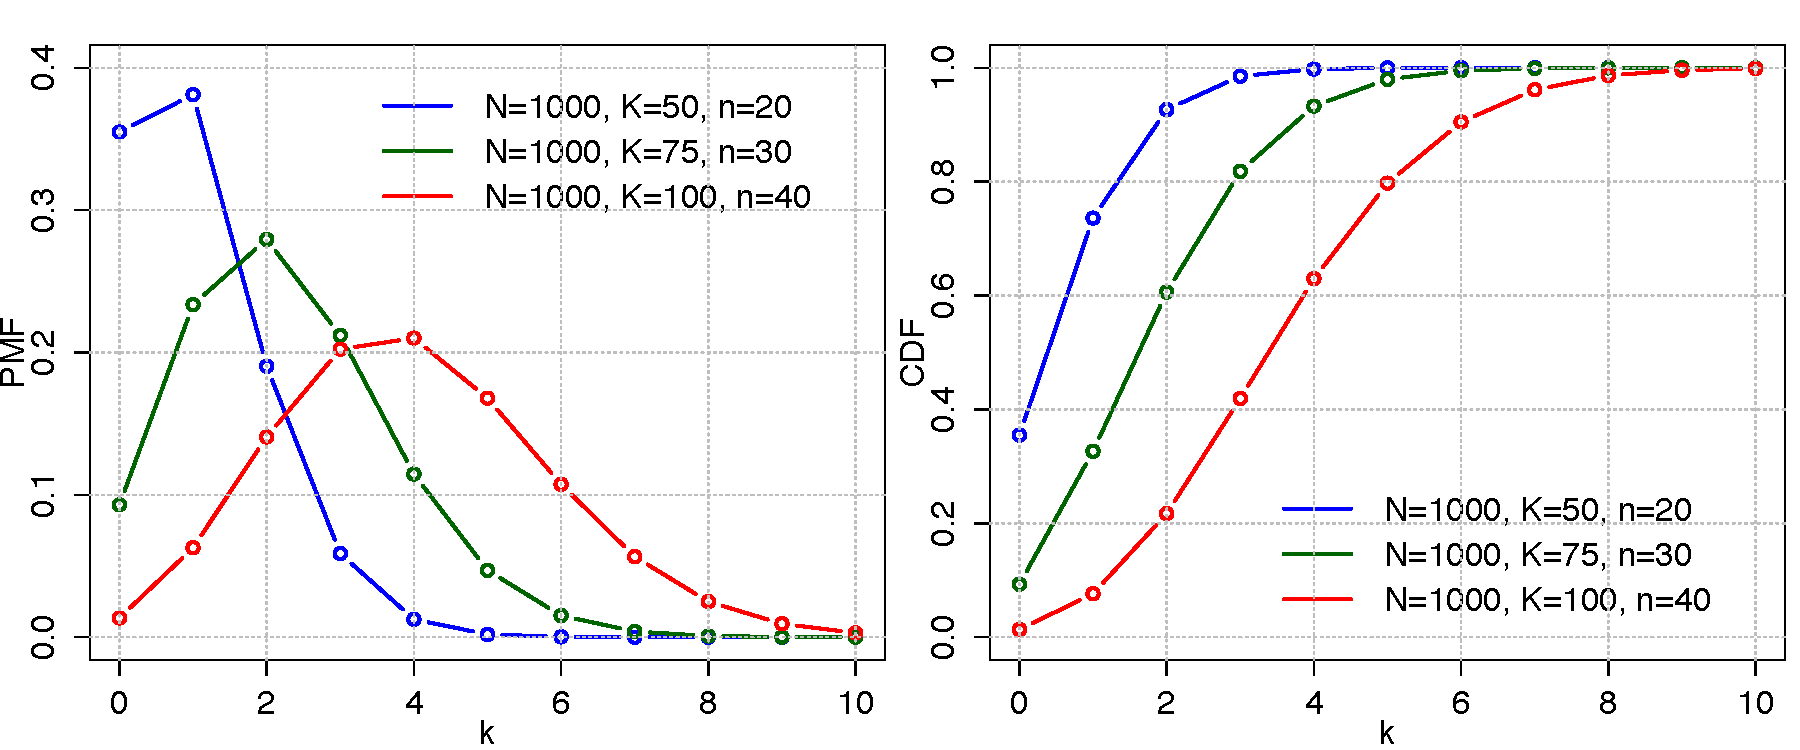
\includegraphics[width=140mm]{pics/Hypergeometric.pdf}
 \caption{Hypergeometric distribution plotted using the provided R code.}
 \label{fig:Hypergeometric}
\end{figure}

\subsubsection*{Parameter: populationSize}

\noindent\begin{tabular}{p{2cm}cl}
\textbf{name} & & population size \\
\textbf{type} & & scalar \\
\textbf{symbol} & & $N$  \\
\textbf{definition} & & $N \in \left\{0,1,2,\dots\right\}$
\end{tabular}
\subsubsection*{Parameter: numberOfSuccesses}

\noindent\begin{tabular}{p{2cm}cl}
\textbf{name} & & number of successes \\
\textbf{type} & & scalar \\
\textbf{symbol} & & $K$  \\
\textbf{definition} & & $K \in \left\{0,1,2,\dots,N\right\} $
\end{tabular}
\subsubsection*{Parameter: numberOfTrials}

\noindent\begin{tabular}{p{2cm}cl}
\textbf{name} & & number of trials \\
\textbf{type} & & scalar \\
\textbf{symbol} & & $n$  \\
\textbf{definition} & & $n \in \left\{0,1,2,\dots,N\right\}$
\end{tabular}
\subsubsection*{Functions}

\smallskip \noindent \hspace{.2cm} \textbf{PMF} 
\begin{equation*}{{{K \choose k} {{N-K} \choose {n-k}}}\over {N \choose n}}\end{equation*}
\smallskip \noindent \hspace{.2cm} \textbf{PMF in R}  
\begin{verbatim}choose(K,k)*choose(M-K,n-k)/choose(M,n)\end{verbatim}
\smallskip \noindent \hspace{.2cm} \textbf{CDF} 
\begin{equation*}1-{{{n \choose {k+1}}{{N-n} \choose {K-k-1}}}\over {N \choose K}} \,_3F_2\!\!\left[\begin{array}{c}1,\ k+1-K,\ k+1-n \\ k+2,\ N+k+2-K-n\end{array};1\right]\end{equation*}
\smallskip \noindent \hspace{.2cm} \textbf{CDF in R} 
\begin{verbatim}cumsum(PMF)\end{verbatim}
\smallskip
\subsubsection*{Characteristics}
\smallskip \noindent \hspace{.2cm} \textbf{Mean} 
\begin{equation*}n {K\over N}\end{equation*}
\smallskip \noindent \hspace{.2cm} \textbf{Mode} 
\begin{equation*}\left \lfloor \frac{(n+1)(K+1)}{N+2} \right \rfloor\end{equation*}
\smallskip \noindent \hspace{.2cm} \textbf{Variance} 
\begin{equation*}n{K\over N}{(N-K)\over N}{N-n\over N-1}\end{equation*}
\smallskip
\section*{InverseBinomial1} 

  \bigskip 

\begin{tabular}{p{2cm}cl}
\textbf{name} & & Inverse Binomial (ID: 0000207)\\ 
 
\textbf{type} & & discrete \\ 

\textbf{variate} & & $x$, scalar \\ 

\textbf{support} & & $x \in  \{0,1,2,3,\dots\}$
\end{tabular}

\begin{figure}[ht!]
\centering
  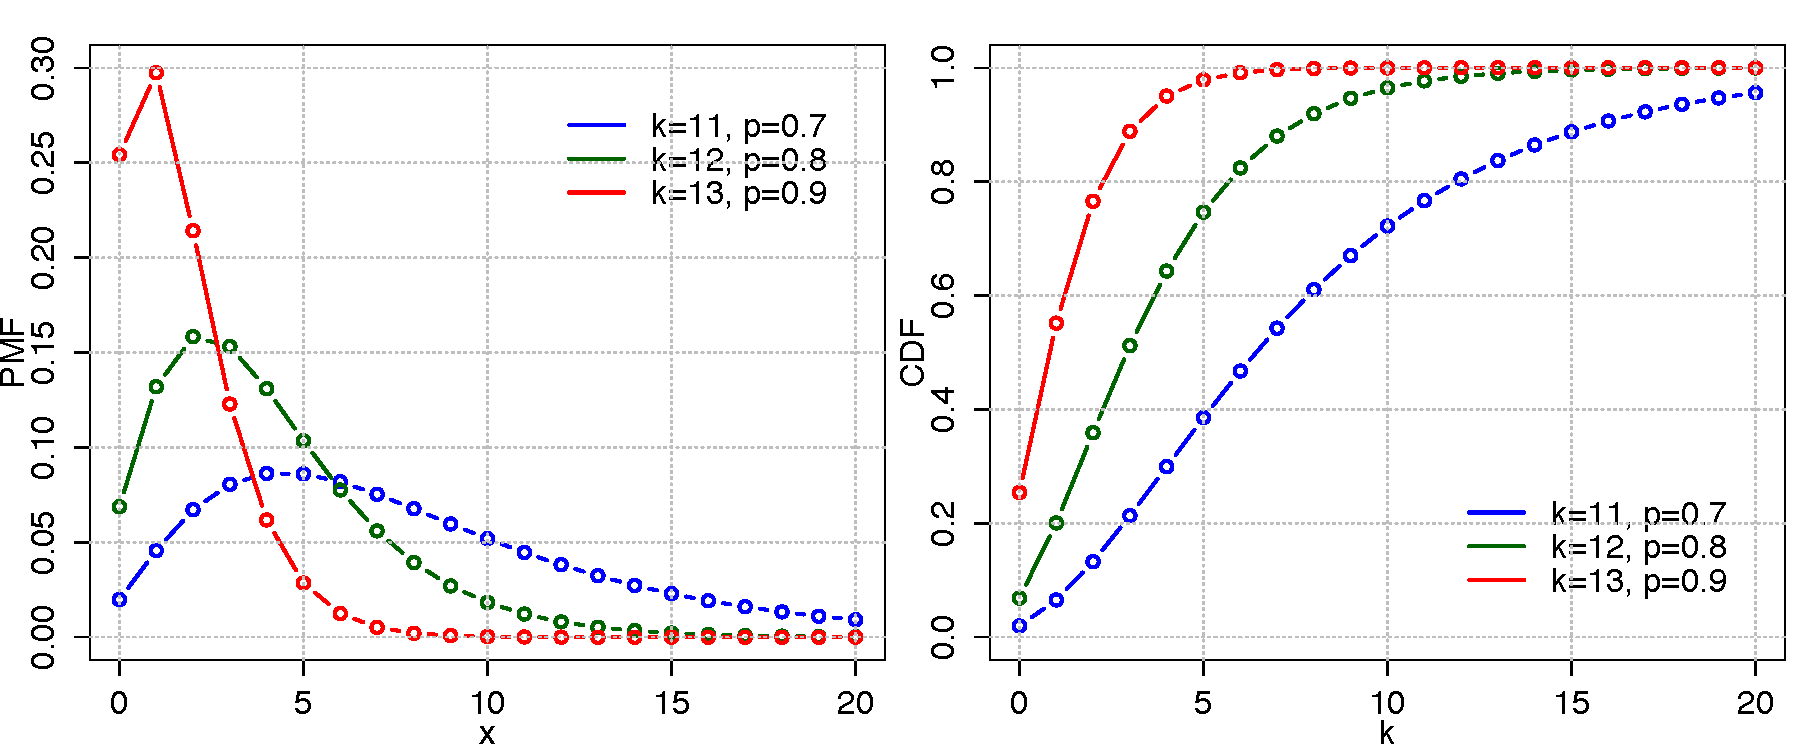
\includegraphics[width=140mm]{pics/InverseBinomial.pdf}
 \caption{InverseBinomial distribution plotted using the provided R code.}
 \label{fig:InverseBinomial}
\end{figure}

\subsubsection*{Parameter: k}

\noindent\begin{tabular}{p{2cm}cl}
\textbf{name} & & - \\
\textbf{type} & & scalar \\
\textbf{symbol} & & $k$  \\
\textbf{definition} & & $k \in \left\{0,1,2,\dots\right\}$
\end{tabular}
\subsubsection*{Parameter: p}

\noindent\begin{tabular}{p{2cm}cl}
\textbf{name} & & - \\
\textbf{type} & & scalar \\
\textbf{symbol} & & $p$  \\
\textbf{definition} & & $1/2 < p < 1$
\end{tabular}
\subsubsection*{Functions}

\smallskip \noindent \hspace{.2cm} \textbf{PMF} 
\begin{equation*}\frac{k \; \Gamma(2x + k)}{\Gamma(x+1) \;\Gamma(x + k + 1)}  \; p^{k+x} (1-p)^x \end{equation*}
\smallskip \noindent \hspace{.2cm} \textbf{PMF in R}  
\begin{verbatim}(k * gamma(2*x+k)) / (gamma(x+1) * gamma(x+k+1)) * p^(x+k) * (1-p)^x\end{verbatim}
\smallskip \noindent \hspace{.2cm} \textbf{CDF} 
\begin{equation*}\Sigma_{i=1}^x f(i), x \in \{0,1,2,...\}
\text { with f the PMF}\end{equation*}
\smallskip \noindent \hspace{.2cm} \textbf{CDF in R}  
\begin{verbatim}
cumsum(PMF)
\end{verbatim}

\smallskip
\subsubsection*{Characteristics}
\smallskip
\section*{InverseGamma1} 

  \bigskip 

\begin{tabular}{p{2cm}cl}
\textbf{name} & & Inverse-Gamma (ID: 0000216)\\ 
 
\textbf{type} & & continuous \\ 

\textbf{variate} & & $x$, scalar \\ 

\textbf{support} & & $x \in (0,+\infty)$
\end{tabular}

\begin{figure}[ht!]
\centering
  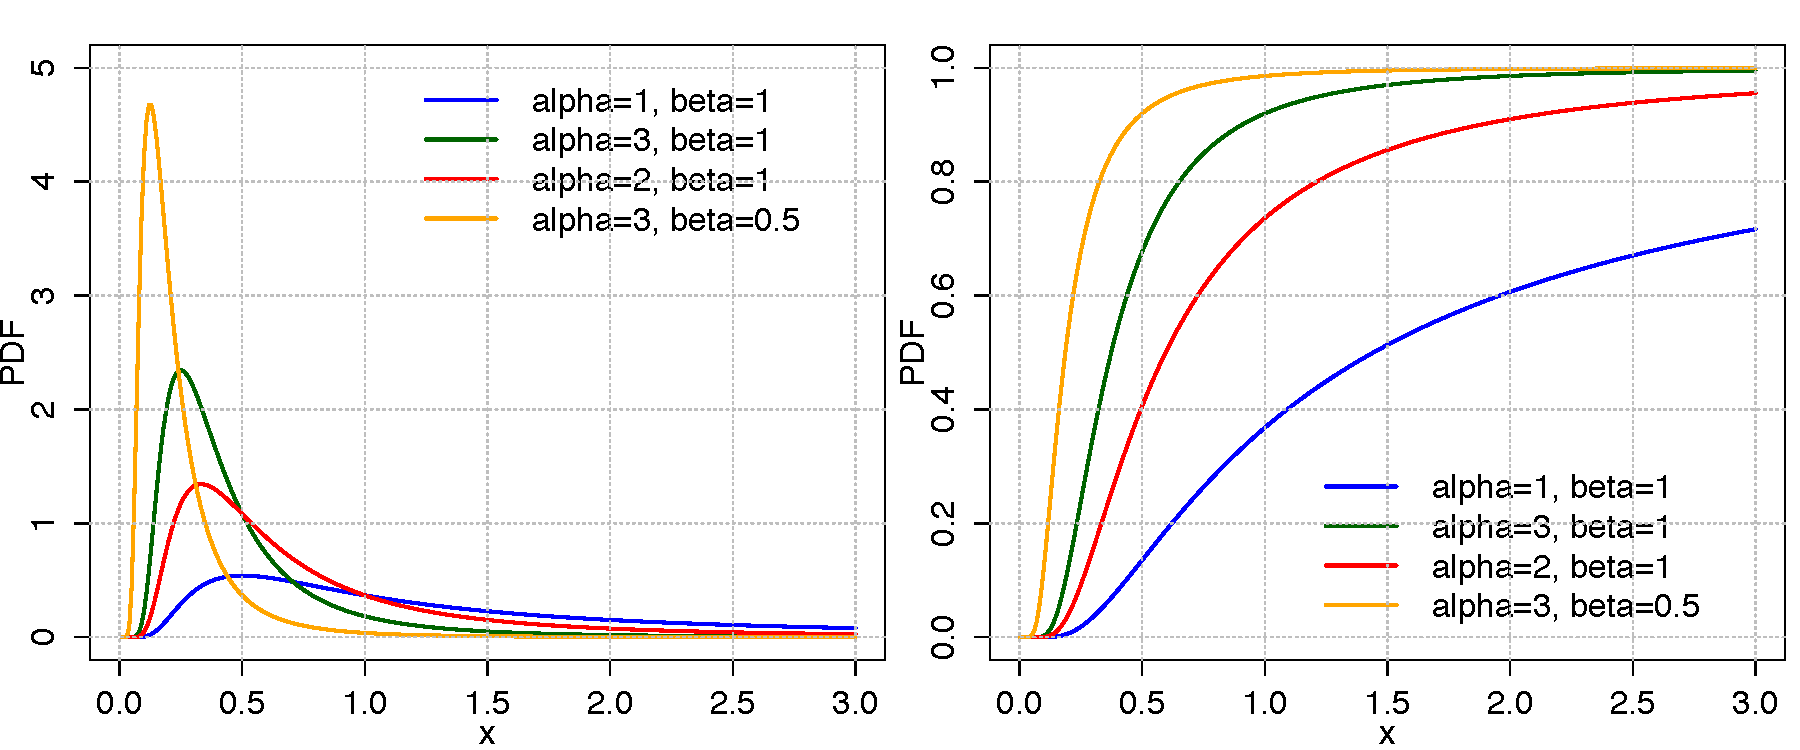
\includegraphics[width=140mm]{pics/InverseGamma.pdf}
 \caption{InverseGamma distribution plotted using the provided R code.}
 \label{fig:InverseGamma}
\end{figure}

\subsubsection*{Parameter: shape}

\noindent\begin{tabular}{p{2cm}cl}
\textbf{name} & & shape \\
\textbf{type} & & scalar \\
\textbf{symbol} & & $\alpha$  \\
\textbf{definition} & & $\alpha>0, \alpha \in  R$
\end{tabular}
\subsubsection*{Parameter: scale}

\noindent\begin{tabular}{p{2cm}cl}
\textbf{name} & & scale \\
\textbf{type} & & scalar \\
\textbf{symbol} & & $\beta$  \\
\textbf{definition} & & $\beta>0, \beta \in  R$
\end{tabular}
\subsubsection*{Functions}

\smallskip \noindent \hspace{.2cm} \textbf{PDF} 
\begin{equation*}\frac{\beta^\alpha}{\Gamma(\alpha)} x^{-\alpha - 1} \exp \left(\frac{-\beta}{x}\right)\end{equation*}
\smallskip \noindent \hspace{.2cm} \textbf{PDF in R}  
\begin{verbatim}beta^alpha/gamma(alpha) * x^(-alpha-1) * exp(-beta/x)\end{verbatim}
\smallskip \noindent \hspace{.2cm} \textbf{CDF} 
\begin{equation*}\frac{\Gamma(\alpha, \beta/x)}{\Gamma(\alpha)}\end{equation*}
\smallskip \noindent \hspace{.2cm} \textbf{CDF in R} 
\begin{verbatim}Igamma(alpha, beta/x, lower=F) / gamma(alpha)\end{verbatim}
\smallskip
\subsubsection*{Characteristics}
\smallskip \noindent \hspace{.2cm} \textbf{Mean} 
\begin{equation*}\frac{\beta}{\alpha-1} \text{ for } \alpha > 1\end{equation*}
\smallskip \noindent \hspace{.2cm} \textbf{Mode} 
\begin{equation*}\frac{\beta}{\alpha + 1}\end{equation*}
\smallskip \noindent \hspace{.2cm} \textbf{Variance} 
\begin{equation*}\frac{\beta^2}{(\alpha-1)^2(\alpha-2)} \text{ for } \alpha > 2\end{equation*}
\smallskip
\section*{InverseGaussian1} 

  \bigskip 

\begin{tabular}{p{2cm}cl}
\textbf{name} & & Inverse Gaussian (ID: 0000226)\\ 
 
\textbf{type} & & continuous \\ 

\textbf{variate} & & $$,  \\ 

\textbf{support} & & $$
\end{tabular}

\begin{figure}[ht!]
\centering
  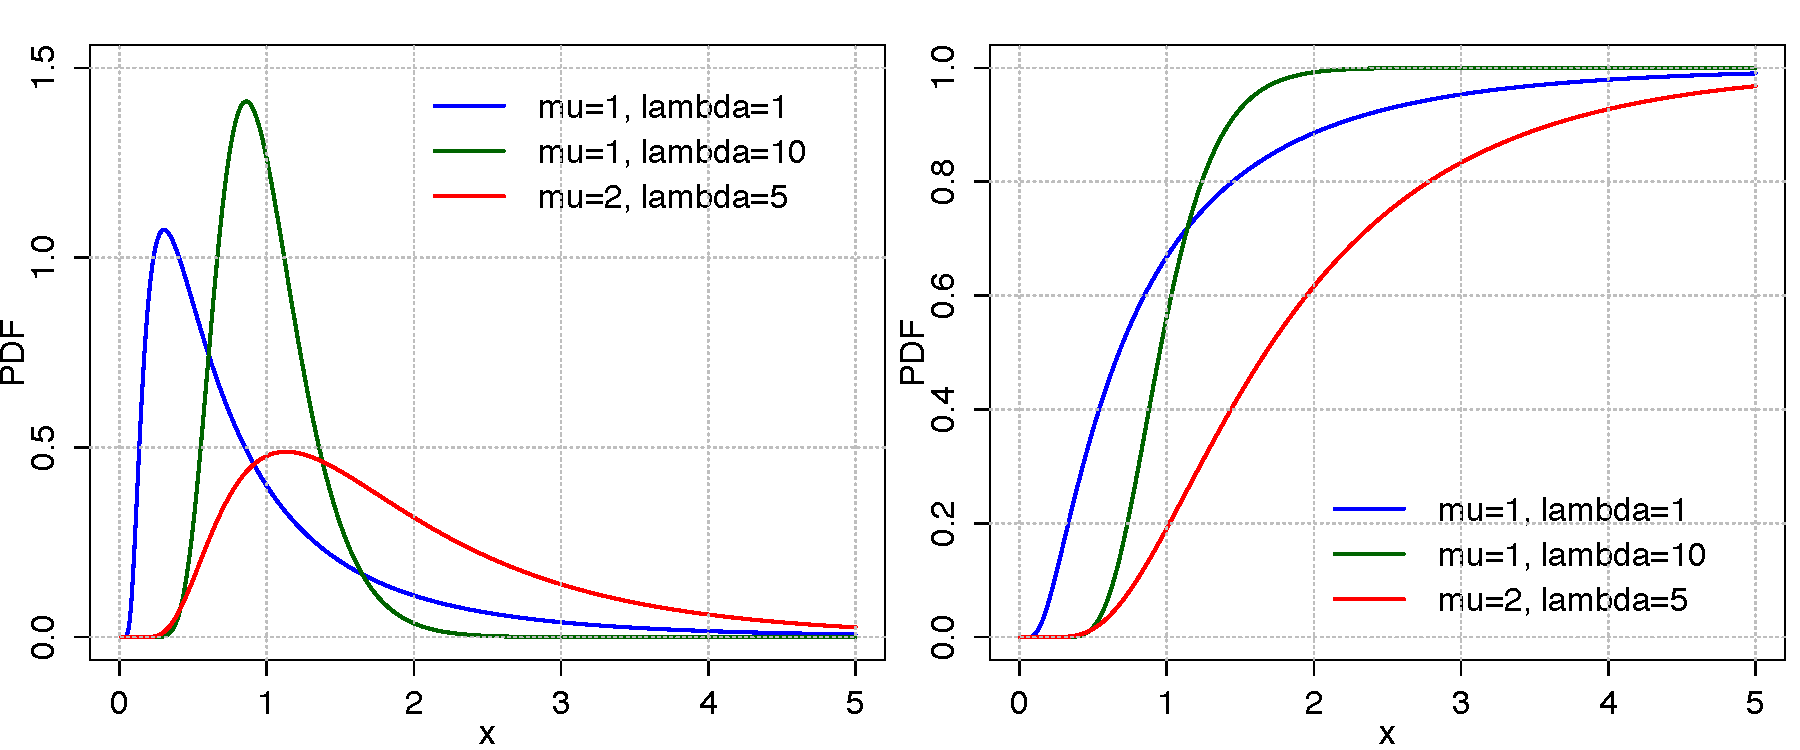
\includegraphics[width=140mm]{pics/InverseGaussian.pdf}
 \caption{InverseGaussian distribution plotted using the provided R code.}
 \label{fig:InverseGaussian}
\end{figure}

\subsubsection*{Parameter: shape}

\noindent\begin{tabular}{p{2cm}cl}
\textbf{name} & & shape \\
\textbf{type} & & scalar \\
\textbf{symbol} & & $\lambda$  \\
\textbf{definition} & & $\lambda > 0$
\end{tabular}
\subsubsection*{Parameter: mean}

\noindent\begin{tabular}{p{2cm}cl}
\textbf{name} & & mean \\
\textbf{type} & & scalar \\
\textbf{symbol} & & $\mu$  \\
\textbf{definition} & & $\mu > 0$
\end{tabular}
\subsubsection*{Functions}

\smallskip \noindent \hspace{.2cm} \textbf{PDF} 
\begin{equation*}\sqrt{\frac{\lambda}{2\pi x^3}} \exp\Big(-\frac{\lambda}{2\mu^2 x}(x-\mu)^2\Big)\end{equation*}
\smallskip \noindent \hspace{.2cm} \textbf{PDF in R}  
\begin{verbatim}sqrt(lambda/(2*pi*x^3) ) * exp(-lambda/(2*mu^2 x) * (x-mu)^2)\end{verbatim}
\smallskip \noindent \hspace{.2cm} \textbf{CDF} 
\begin{equation*}\Phi\left(\sqrt{\frac{\lambda}{x}} \left(\frac{x}{\mu}-1 \right)\right) +\exp\left(\frac{2 \lambda}{\mu}\right) \Phi\left(-\sqrt{\frac{\lambda}{x}}\left(\frac{x}{\mu}+1 \right)\right)\end{equation*}
\smallskip \noindent \hspace{.2cm} \textbf{CDF in R} 
\begin{verbatim}pnorm(sqrt(lambda/x) * (x/mu-1)) + exp(2*lambda/mu) * pnorm(-sqrt(lambda/x) * (x/mu+1))\end{verbatim}
\smallskip
\subsubsection*{Characteristics}
\smallskip
\section*{InverseWishart1} 

  \bigskip 

\begin{tabular}{p{2cm}cl}
\textbf{name} & & Inverse-Wishart (ID: 0000235)\\ 
 
\textbf{type} & & continuous \\ 

\textbf{variate} & & $X$, matrix \\ 

\textbf{support} & & $X(p \times p) - \text{positive-definite matrix}$
\end{tabular}

%\begin{figure}[ht!]
%\centering
%  \includegraphics[width=140mm]{pics/InverseWishart.pdf}
% \caption{InverseWishart distribution plotted using the provided R code.}
% \label{fig:InverseWishart}
%\end{figure}

\subsubsection*{Parameter: scaleMatrix}

\noindent\begin{tabular}{p{2cm}cl}
\textbf{name} & & scale matrix \\
\textbf{type} & & matrix \\
\textbf{symbol} & & $\Psi$  \\
\textbf{definition} & & $\Psi > 0, \text{positive-definite matrix}$
\end{tabular}
\subsubsection*{Parameter: degreesOfFreedom}

\noindent\begin{tabular}{p{2cm}cl}
\textbf{name} & & degrees of freedom \\
\textbf{type} & & scalar \\
\textbf{symbol} & & $\nu$  \\
\textbf{definition} & & $\nu > p-1, \nu \in  R$
\end{tabular}
\subsubsection*{Functions}

\smallskip \noindent \hspace{.2cm} \textbf{PDF} 
\begin{equation*}\frac{\left|\Psi\right|^{\frac{\nu}{2}}}{2^{\frac{\nu p}{2}}\Gamma_p(\frac{\nu}{2})} \left|X\right|^{-\frac{\nu+p+1}{2}}e^{-\frac{1}{2}\text{tr}(\Psi X^{-1})}\end{equation*}
\smallskip \noindent \hspace{.2cm} \textbf{CDF} 
\begin{equation*}-\end{equation*}
\smallskip
\subsubsection*{Characteristics}
\smallskip \noindent \hspace{.2cm} \textbf{Mean} 
\begin{equation*}\frac{\Psi}{\nu - p - 1} \text{ for }\nu > p + 1\end{equation*}
\smallskip \noindent \hspace{.2cm} \textbf{Mode} 
\begin{equation*}\frac{\Psi}{\nu + p + 1}\end{equation*}
\smallskip
\section*{Laplace1} 

  \bigskip 

\begin{tabular}{p{2cm}cl}
\textbf{name} & & Laplace 1 (ID: 0000245)\\ 
 
\textbf{type} & & continuous \\ 

\textbf{variate} & & $x$, scalar \\ 

\textbf{support} & & $x \in (-\infty,+\infty)$
\end{tabular}

\begin{figure}[ht!]
\centering
  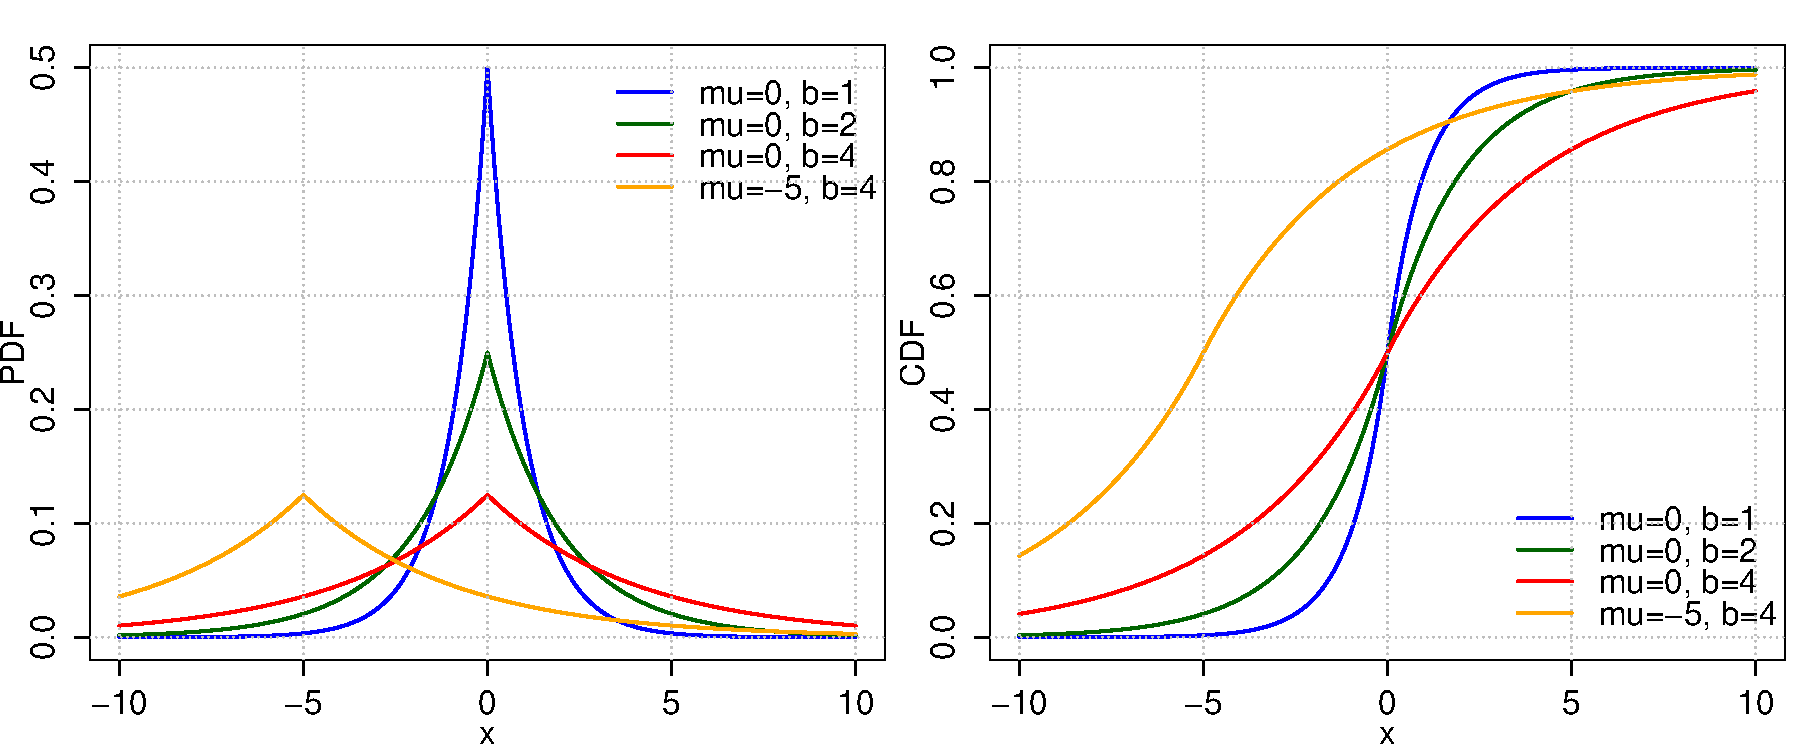
\includegraphics[width=140mm]{pics/Laplace1.pdf}
 \caption{Laplace1 distribution plotted using the provided R code.}
 \label{fig:Laplace1}
\end{figure}

\subsubsection*{Parameter: location}

\noindent\begin{tabular}{p{2cm}cl}
\textbf{name} & & location \\
\textbf{type} & & scalar \\
\textbf{symbol} & & $\mu$  \\
\textbf{definition} & & $\mu \in R$
\end{tabular}
\subsubsection*{Parameter: scale}

\noindent\begin{tabular}{p{2cm}cl}
\textbf{name} & & scale \\
\textbf{type} & & scalar \\
\textbf{symbol} & & $b$  \\
\textbf{definition} & & $b > 0, b \in R$
\end{tabular}
\subsubsection*{Functions}

\smallskip \noindent \hspace{.2cm} \textbf{PDF} 
\begin{equation*}\frac{1}{2\,b} \exp \left(-\frac{|x-\mu|}b \right)\end{equation*}
\smallskip \noindent \hspace{.2cm} \textbf{PDF in R}  
\begin{verbatim}1/(2*b) * exp(- abs(x-mu)/b )\end{verbatim}
\smallskip \noindent \hspace{.2cm} \textbf{CDF} 
\begin{equation*}\begin{cases}
      \frac12 \exp \left( \frac{x-\mu}{b} \right) & \mbox{if }x < \mu \\
          1-\frac12 \exp \left( -\frac{x-\mu}{b} \right) & \mbox{if }x \geq \mu
       \end{cases}\end{equation*}
\smallskip \noindent \hspace{.2cm} \textbf{CDF in R} 
\begin{verbatim}1/2 * exp( (x-mu)/b ) for x < mu
1- 1/2 * exp( -(x-mu)/b ) x >= mu\end{verbatim}
\smallskip
\subsubsection*{Characteristics}
\smallskip \noindent \hspace{.2cm} \textbf{Mean} 
\begin{equation*}\mu\end{equation*}
\smallskip \noindent \hspace{.2cm} \textbf{Median} 
\begin{equation*}\mu\end{equation*}
\smallskip \noindent \hspace{.2cm} \textbf{Mode} 
\begin{equation*}\mu\end{equation*}
\smallskip \noindent \hspace{.2cm} \textbf{Variance} 
\begin{equation*}2 b^2\end{equation*}
\smallskip
\section*{Laplace2} 

  \bigskip 

\begin{tabular}{p{2cm}cl}
\textbf{name} & & Laplace 2 (ID: 0000256)\\ 
 
\textbf{type} & & continuous \\ 

\textbf{variate} & & $x$, scalar \\ 

\textbf{support} & & $x \in (-\infty,+\infty)$
\end{tabular}

\begin{figure}[ht!]
\centering
  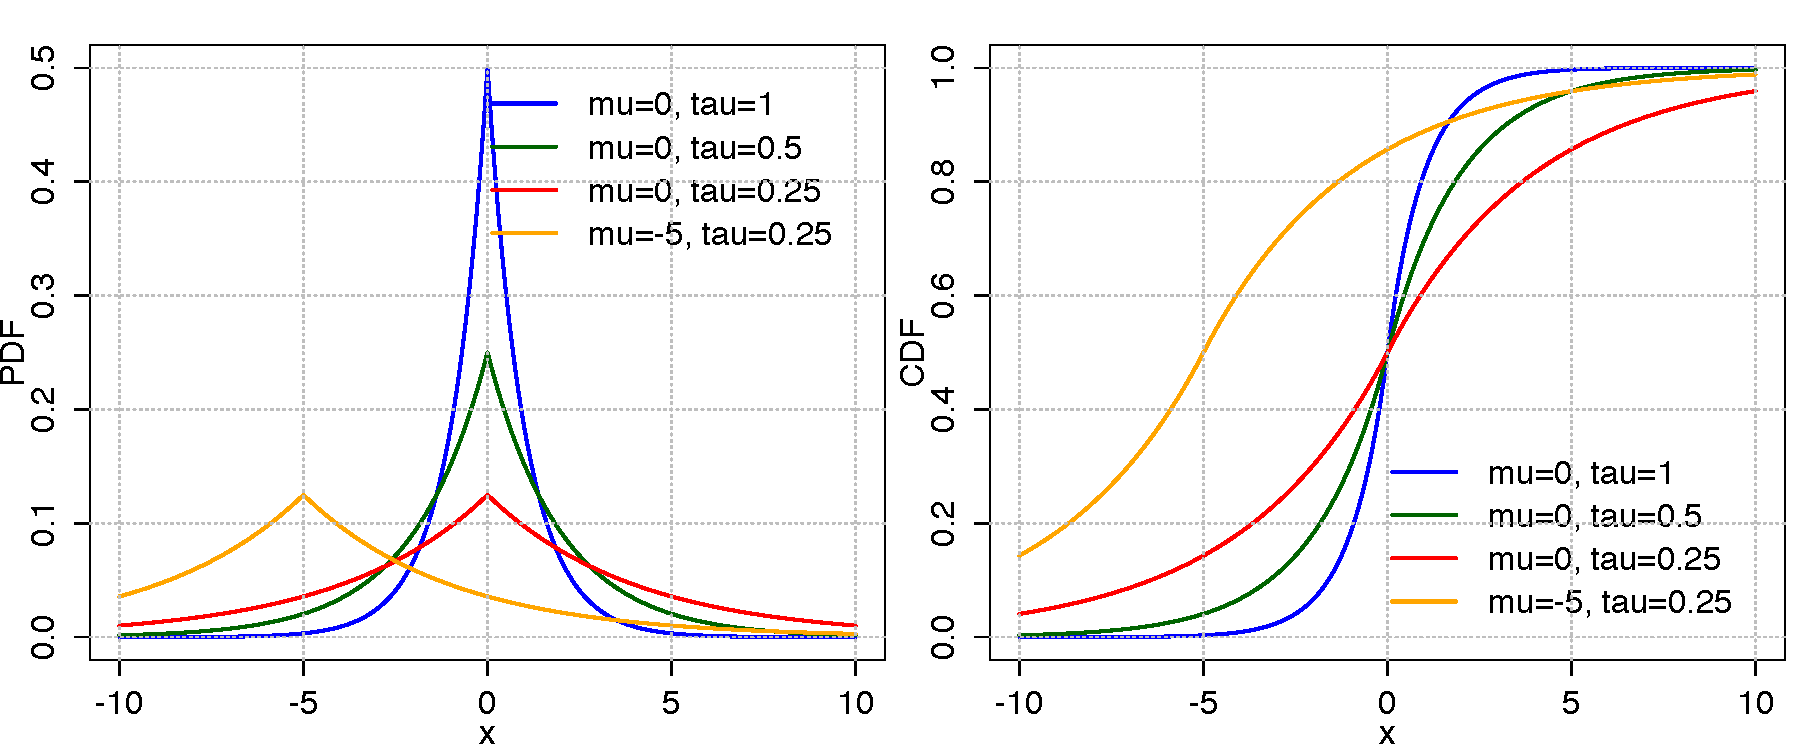
\includegraphics[width=140mm]{pics/Laplace2.pdf}
 \caption{Laplace2 distribution plotted using the provided R code.}
 \label{fig:Laplace2}
\end{figure}

\subsubsection*{Parameter: location}

\noindent\begin{tabular}{p{2cm}cl}
\textbf{name} & & location \\
\textbf{type} & & scalar \\
\textbf{symbol} & & $\mu$  \\
\textbf{definition} & & $\mu \in R$
\end{tabular}
\subsubsection*{Parameter: tau}

\noindent\begin{tabular}{p{2cm}cl}
\textbf{name} & & precision \\
\textbf{type} & & scalar \\
\textbf{symbol} & & $\tau$  \\
\textbf{definition} & & $\tau > 0, \tau \in R$
\end{tabular}
\subsubsection*{Functions}

\smallskip \noindent \hspace{.2cm} \textbf{PDF} 
\begin{equation*}\frac{\tau}{2} \exp \left(-\tau|x-\mu| \right)\end{equation*}
\smallskip \noindent \hspace{.2cm} \textbf{PDF in R}  
\begin{verbatim}tau/2 * exp(-tau * abs(x-mu))\end{verbatim}
\smallskip \noindent \hspace{.2cm} \textbf{CDF} 
\begin{equation*}\begin{cases}
\frac12 \exp \left( \tau (x-\mu) \right) & \mbox{if }x < \mu \\
1-\frac12 \exp \left( -\tau (x-\mu) \right) & \mbox{if }x \geq \mu
\end{cases}\end{equation*}
\smallskip \noindent \hspace{.2cm} \textbf{CDF in R} 
\begin{verbatim}1/2 * exp( tau*(x-mu) ) for x < mu
1- 1/2 * exp( -tau*(x-mu) ) x >= mu\end{verbatim}
\smallskip
\subsubsection*{Characteristics}
\smallskip \noindent \hspace{.2cm} \textbf{Mean} 
\begin{equation*}\mu\end{equation*}
\smallskip \noindent \hspace{.2cm} \textbf{Variance} 
\begin{equation*}2 / \tau^2\end{equation*}
\smallskip
\section*{Logistic1} 

  \bigskip 

\begin{tabular}{p{2cm}cl}
\textbf{name} & & Logistic (ID: 0000268)\\ 
 
\textbf{type} & & continuous \\ 

\textbf{variate} & & $x$, scalar \\ 

\textbf{support} & & $x \in (-\infty,+\infty)$
\end{tabular}

\begin{figure}[ht!]
\centering
  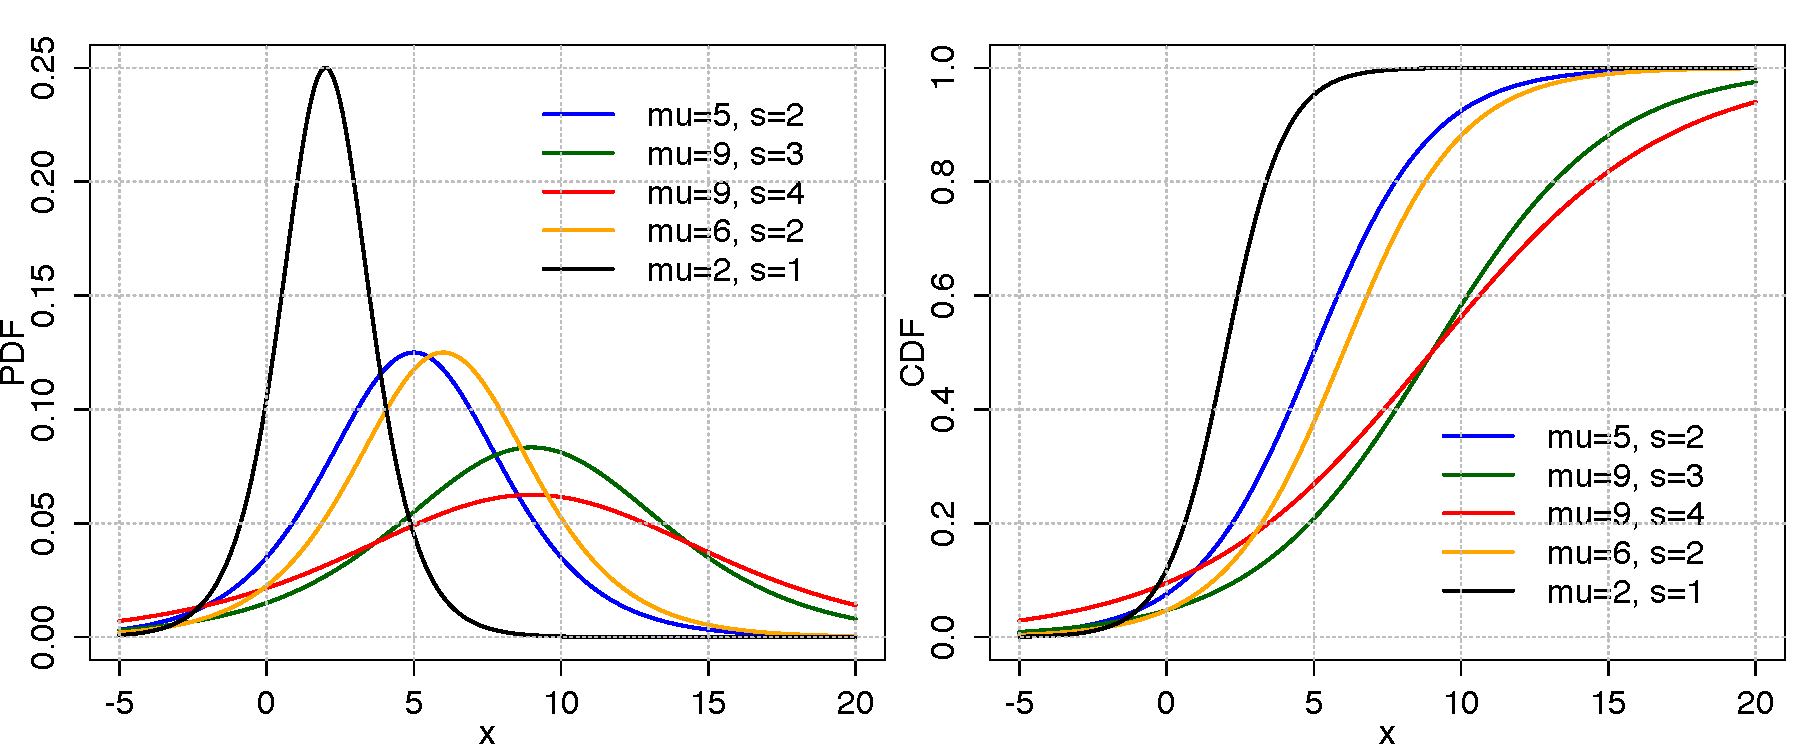
\includegraphics[width=140mm]{pics/Logistic.pdf}
 \caption{Logistic distribution plotted using the provided R code.}
 \label{fig:Logistic}
\end{figure}

\subsubsection*{Parameter: location}

\noindent\begin{tabular}{p{2cm}cl}
\textbf{name} & & location \\
\textbf{type} & & scalar \\
\textbf{symbol} & & $\mu$  \\
\textbf{definition} & & $\mu \in R$
\end{tabular}
\subsubsection*{Parameter: scale}

\noindent\begin{tabular}{p{2cm}cl}
\textbf{name} & & scale \\
\textbf{type} & & scalar \\
\textbf{symbol} & & $s$  \\
\textbf{definition} & & $s > 0, s \in R$
\end{tabular}
\subsubsection*{Functions}

\smallskip \noindent \hspace{.2cm} \textbf{PDF} 
\begin{equation*}\frac{e^{-\frac{x-\mu}{s}}} {s\left(1+e^{-\frac{x-\mu}{s}}\right)^2}\end{equation*}
\smallskip \noindent \hspace{.2cm} \textbf{PDF in R}  
\begin{verbatim}exp(-(x-mu)/s) / (s*(1+exp(-(x-mu)/s))^2)\end{verbatim}
\smallskip \noindent \hspace{.2cm} \textbf{CDF} 
\begin{equation*}\frac{1}{1+e^{-\frac{x-\mu}{s}}}\end{equation*}
\smallskip \noindent \hspace{.2cm} \textbf{CDF in R} 
\begin{verbatim}1/(1+exp(-(x-mu)/s))\end{verbatim}
\smallskip
\subsubsection*{Characteristics}
\smallskip \noindent \hspace{.2cm} \textbf{Mean} 
\begin{equation*}\mu\end{equation*}
\smallskip \noindent \hspace{.2cm} \textbf{Median} 
\begin{equation*}\mu\end{equation*}
\smallskip \noindent \hspace{.2cm} \textbf{Mode} 
\begin{equation*}\mu\end{equation*}
\smallskip \noindent \hspace{.2cm} \textbf{Variance} 
\begin{equation*}\frac{s^2 \pi^2}{3}\end{equation*}
\smallskip

\section*{LogLogistic} 

  \bigskip 

\begin{tabular}{p{2cm}cl}
\textbf{name} & & Log-Logistic (ID: 0000278)\\ 
 
\textbf{type} & & continuous \\ 

\textbf{variate} & & $x$, scalar \\ 

\textbf{support} & & $x \in [0,+\infty)$
\end{tabular}

\begin{figure}[ht!]
\centering
  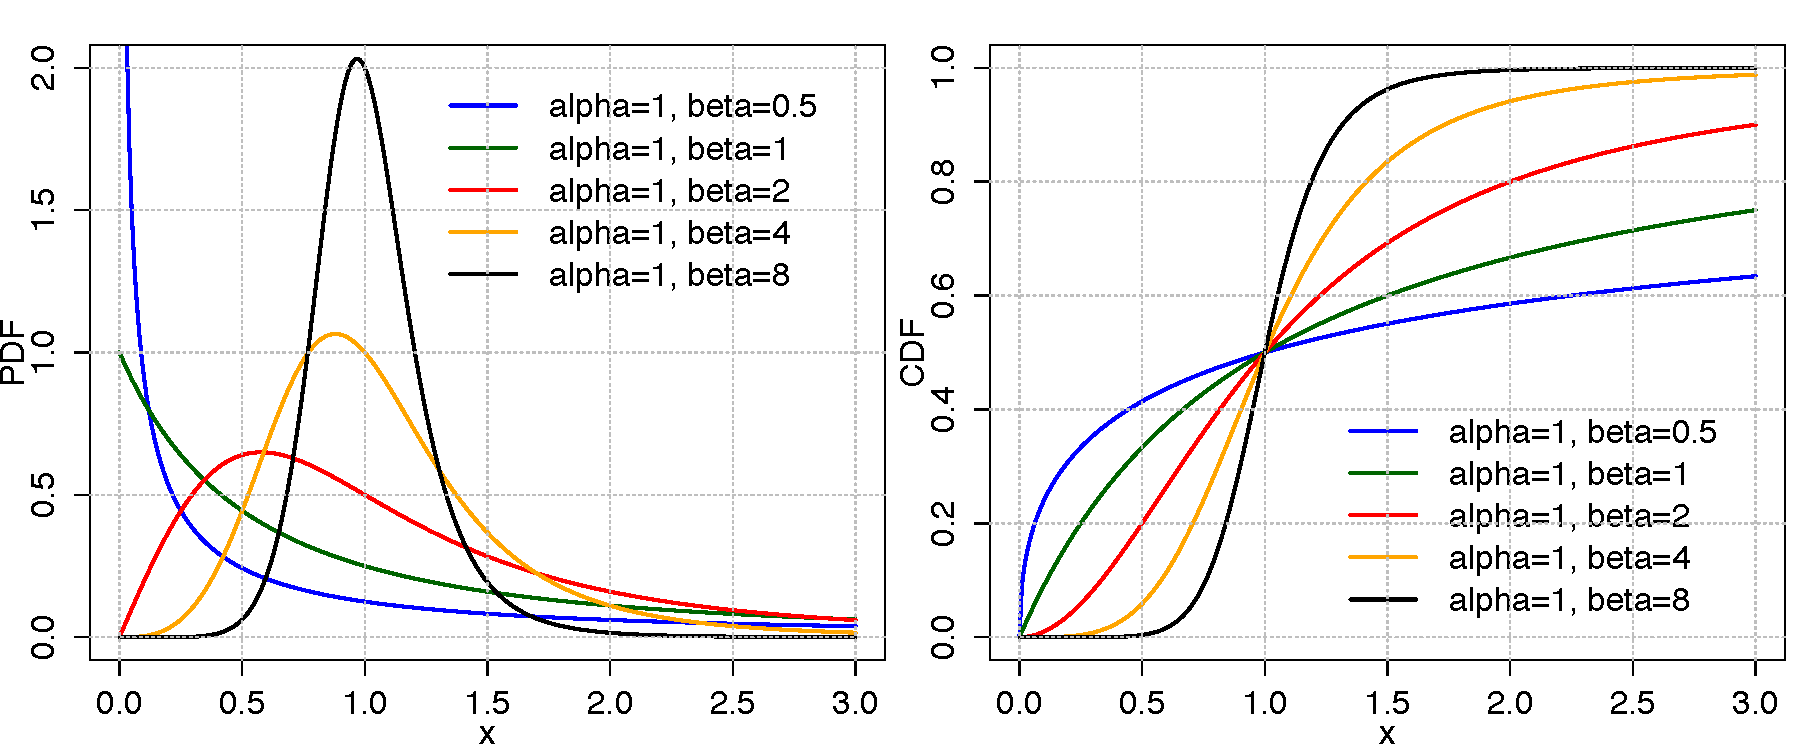
\includegraphics[width=140mm]{pics/LogLogistic.pdf}
 \caption{LogLogistic distribution plotted using the provided R code.}
 \label{fig:LogLogistic}
\end{figure}

\subsubsection*{Parameter: scale}

\noindent\begin{tabular}{p{2cm}cl}
\textbf{name} & & scale \\
\textbf{type} & & scalar \\
\textbf{symbol} & & $\alpha$  \\
\textbf{definition} & & $\alpha > 0$
\end{tabular}
\subsubsection*{Parameter: shape}

\noindent\begin{tabular}{p{2cm}cl}
\textbf{name} & & shape \\
\textbf{type} & & scalar \\
\textbf{symbol} & & $\beta$  \\
\textbf{definition} & & $\beta > 0$
\end{tabular}
\subsubsection*{Functions}

\smallskip \noindent \hspace{.2cm} \textbf{PDF} 
\begin{equation*}\frac{(\beta/\alpha)(x/\alpha)^{\beta-1}}{(1+(x/\alpha)^\beta)^2}\end{equation*}
\smallskip \noindent \hspace{.2cm} \textbf{PDF in R}  
\begin{verbatim}(beta/alpha)*(x/alpha)^(beta-1) / (1+(x/alpha)^beta)^2\end{verbatim}
\smallskip \noindent \hspace{.2cm} \textbf{CDF} 
\begin{equation*}\frac{1}{1+(x/\alpha)^{-\beta}}\end{equation*}
\smallskip \noindent \hspace{.2cm} \textbf{CDF in R} 
\begin{verbatim}1 / (1+(x/alpha)^(-beta))\end{verbatim}
\smallskip
\subsubsection*{Characteristics}
\smallskip \noindent \hspace{.2cm} \textbf{Mean} 
\begin{equation*}\frac{\alpha \pi/\beta}{\sin(\pi/\beta)} \text{ if } \beta>1, \text{ else undefined}\end{equation*}
\smallskip \noindent \hspace{.2cm} \textbf{Median} 
\begin{equation*}\alpha\end{equation*}
\smallskip \noindent \hspace{.2cm} \textbf{Mode} 
\begin{equation*}\alpha \Big(\frac{\beta-1}{\beta+1}\Big)^{1/\beta} \text{ if } \beta>1, 0 \text{ otherwise}\end{equation*}
\smallskip \noindent \hspace{.2cm} \textbf{Variance} 
\begin{equation*}\alpha^2 \Big(\frac{2\pi/\beta}{\sin(2\pi/\beta)} - \frac{(\pi/\beta)^2}{\sin^2(\pi/\beta)} \Big), \text{ for } \beta>2\end{equation*}
\smallskip
\section*{LogNormal1} 

  \bigskip 

\begin{tabular}{p{2cm}cl}
\textbf{name} & & Log-Normal 1 (ID: 0000289)\\ 
 
\textbf{type} & & continuous \\ 

\textbf{variate} & & $x$, scalar \\ 

\textbf{support} & & $x \in (0,+\infty)$
\end{tabular}

\begin{figure}[ht!]
\centering
  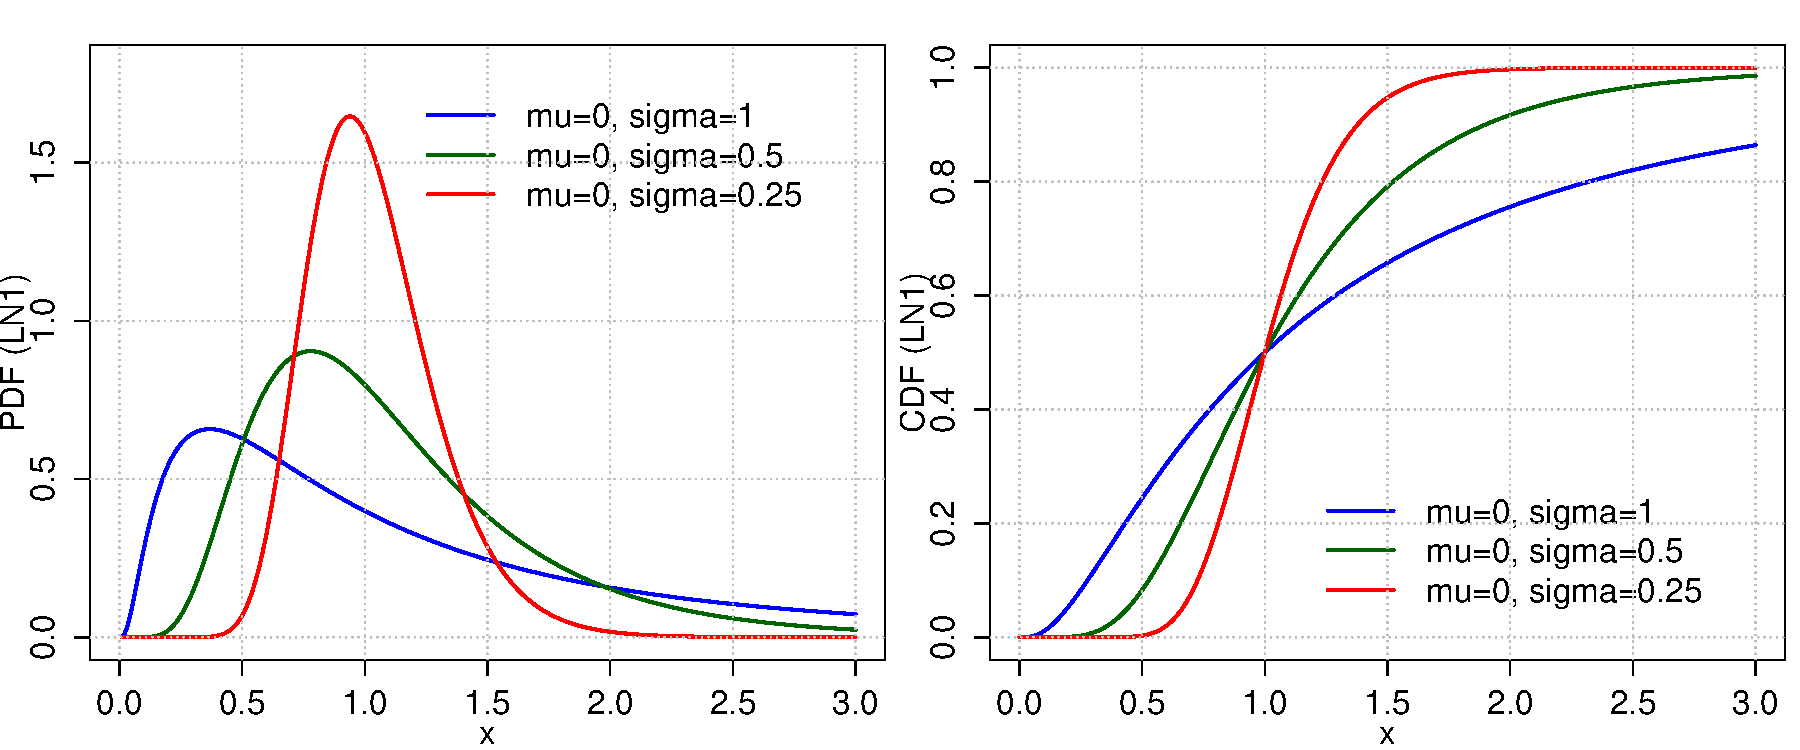
\includegraphics[width=140mm]{pics/LogNormal1.pdf}
 \caption{LogNormal1 distribution plotted using the provided R code.}
 \label{fig:LogNormal1}
\end{figure}

\subsubsection*{Parameter: meanLog}

\noindent\begin{tabular}{p{2cm}cl}
\textbf{name} & & mean of log(x) \\
\textbf{type} & & scalar \\
\textbf{symbol} & & $\mu$  \\
\textbf{definition} & & $\mu \in R$
\end{tabular}
\subsubsection*{Parameter: stdevLog}

\noindent\begin{tabular}{p{2cm}cl}
\textbf{name} & & shape \\
\textbf{type} & & scalar \\
\textbf{symbol} & & $\sigma$  \\
\textbf{definition} & & $\sigma > 0$
\end{tabular}
\subsubsection*{Functions}

\smallskip \noindent \hspace{.2cm} \textbf{PDF} 
\begin{equation*}\frac{1}{x\sigma\sqrt{2\pi}}\ e^{-\frac{\left(\ln x-\mu\right)^2}{2\sigma^2}}\end{equation*}
\smallskip \noindent \hspace{.2cm} \textbf{PDF in R}  
\begin{verbatim}1/(x*sigma*sqrt(2*pi)) * exp((-(log(x)-mu)^2)/(2*sigma^2))\end{verbatim}
\smallskip \noindent \hspace{.2cm} \textbf{CDF} 
\begin{equation*}\frac12 + \frac12\,\text{erf}\Big[\frac{\ln x-\mu}{\sqrt{2}\sigma}\Big]\end{equation*}
\smallskip \noindent \hspace{.2cm} \textbf{CDF in R} 
\begin{verbatim}1/2 + 1/2 *erf( (log(x)-mu)/(sqrt(2)*sigma) )\end{verbatim}
\smallskip
\subsubsection*{Characteristics}
\smallskip \noindent \hspace{.2cm} \textbf{Mean} 
\begin{equation*}e^{\mu+\sigma^2/2}\end{equation*}
\smallskip \noindent \hspace{.2cm} \textbf{Median} 
\begin{equation*}e^{\mu}\end{equation*}
\smallskip \noindent \hspace{.2cm} \textbf{Mode} 
\begin{equation*}e^{\mu-\sigma^2}\end{equation*}
\smallskip \noindent \hspace{.2cm} \textbf{Variance} 
\begin{equation*}(e^{\sigma^2}\!\!-1) e^{2\mu+\sigma^2}\end{equation*}
\smallskip
\section*{LogNormal2} 

  \bigskip 

\begin{tabular}{p{2cm}cl}
\textbf{name} & & Log-Normal 2 (ID: 0000299)\\ 
 
\textbf{type} & & continuous \\ 

\textbf{variate} & & $x$, scalar \\ 

\textbf{support} & & $x \in (0,+\infty)$
\end{tabular}

\begin{figure}[ht!]
\centering
  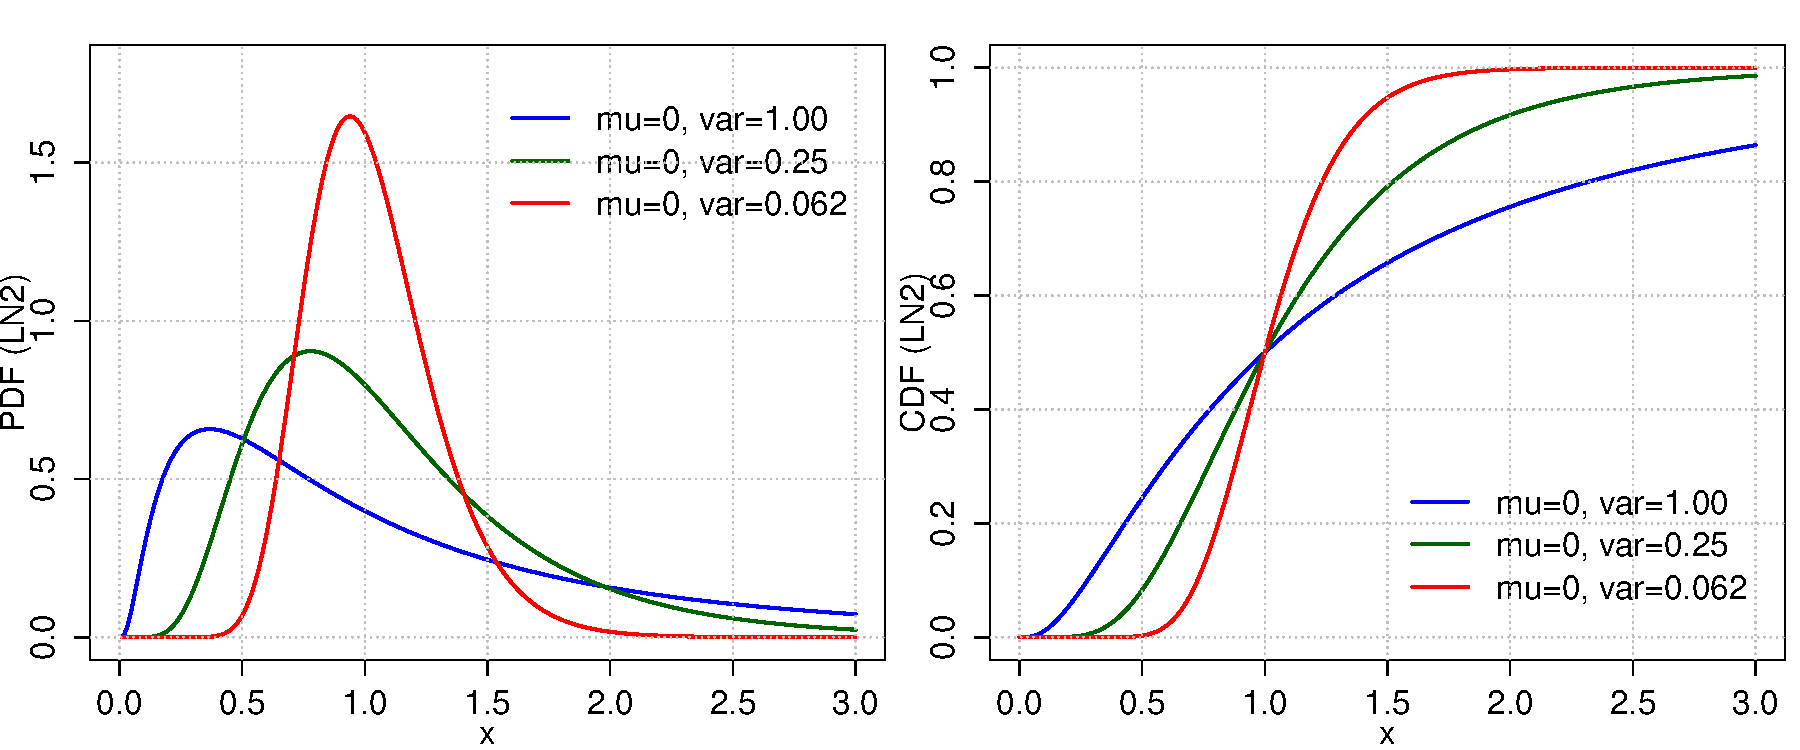
\includegraphics[width=140mm]{pics/LogNormal2.pdf}
 \caption{LogNormal2 distribution plotted using the provided R code.}
 \label{fig:LogNormal2}
\end{figure}

\subsubsection*{Parameter: meanLog}

\noindent\begin{tabular}{p{2cm}cl}
\textbf{name} & & mean of log(x) \\
\textbf{type} & & scalar \\
\textbf{symbol} & & $\mu$  \\
\textbf{definition} & & $\mu \in R$
\end{tabular}
\subsubsection*{Parameter: varLog}

\noindent\begin{tabular}{p{2cm}cl}
\textbf{name} & & shape \\
\textbf{type} & & scalar \\
\textbf{symbol} & & $v$  \\
\textbf{definition} & & $v > 0$
\end{tabular}
\subsubsection*{Functions}

\smallskip \noindent \hspace{.2cm} \textbf{PDF} 
\begin{equation*}\frac{1}{x\sqrt{v}\sqrt{2\pi}}\ e^{-\frac{\left(\ln x-\mu\right)^2}{2 v}}\end{equation*}
\smallskip \noindent \hspace{.2cm} \textbf{PDF in R}  
\begin{verbatim}1/(x*sqrt(v)*sqrt(2*pi)) * exp(-(ln(x)-mu)^2/(2*v))\end{verbatim}
\smallskip \noindent \hspace{.2cm} \textbf{CDF} 
\begin{equation*}\frac12 + \frac12\,\text{erf}\Big[\frac{\ln x-\mu}{\sqrt{2}\sqrt{var}}\Big]\end{equation*}
\smallskip \noindent \hspace{.2cm} \textbf{CDF in R} 
\begin{verbatim}1/2 + 1/2 * erf( (log(x)-mu) / (sqrt(2)*sqrt(var)) )\end{verbatim}
\smallskip
\subsubsection*{Characteristics}
\smallskip
\section*{LogNormal3} 

  \bigskip 

\begin{tabular}{p{2cm}cl}
\textbf{name} & & Log-Normal 3 (ID: 0000309)\\ 
 
\textbf{type} & & continuous \\ 

\textbf{variate} & & $x$, scalar \\ 

\textbf{support} & & $x \in (0,+\infty)$
\end{tabular}

\begin{figure}[ht!]
\centering
  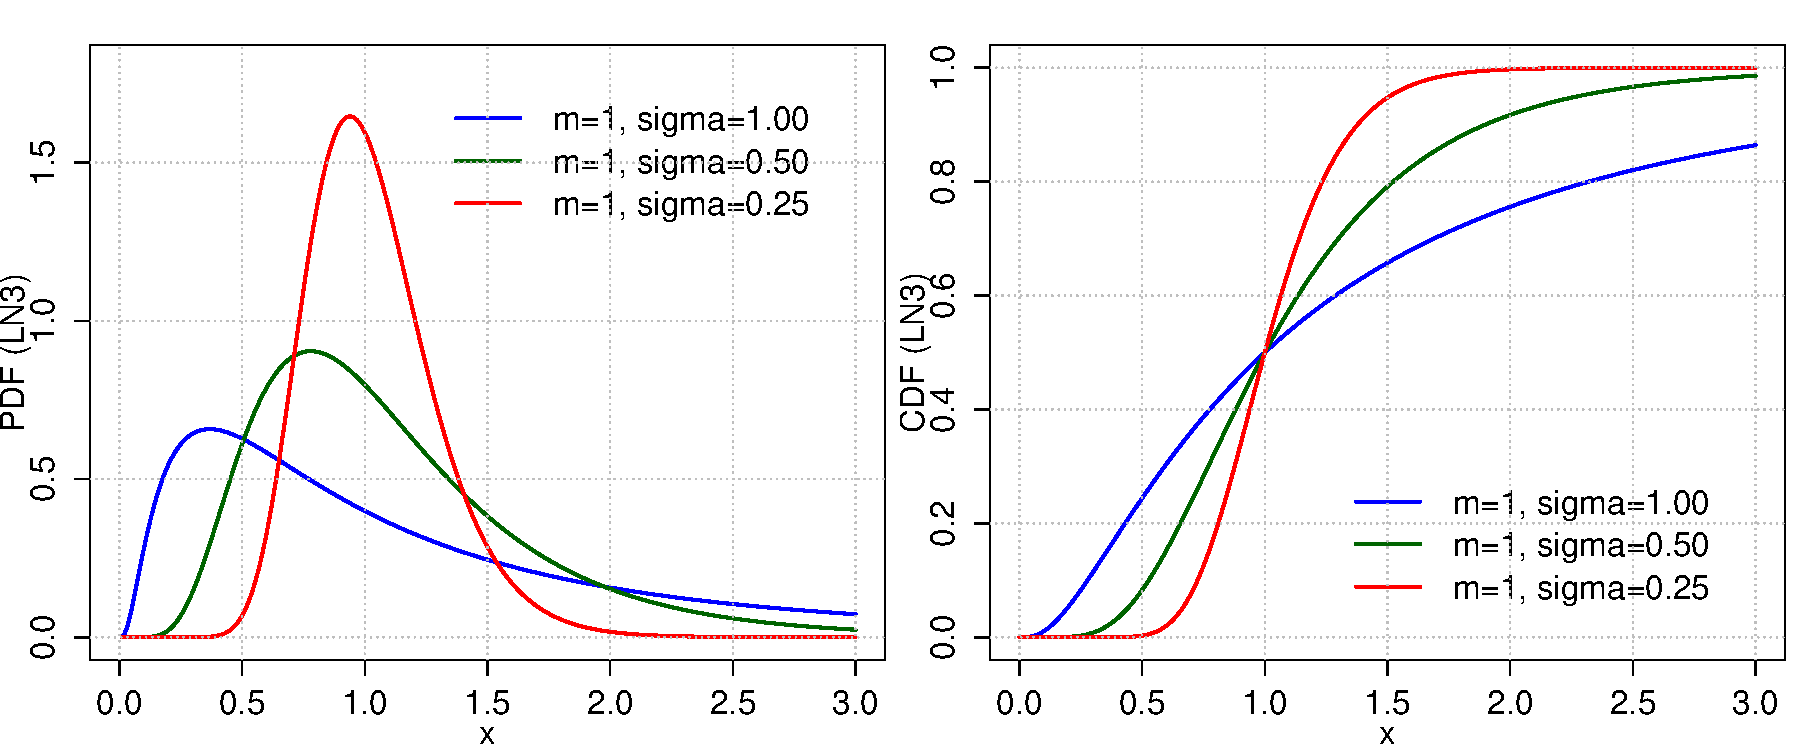
\includegraphics[width=140mm]{pics/LogNormal3.pdf}
 \caption{LogNormal3 distribution plotted using the provided R code.}
 \label{fig:LogNormal3}
\end{figure}

\subsubsection*{Parameter: median}

\noindent\begin{tabular}{p{2cm}cl}
\textbf{name} & & median / geometric mean \\
\textbf{type} & & scalar \\
\textbf{symbol} & & $m$  \\
\textbf{definition} & & $m>0$
\end{tabular}
\subsubsection*{Parameter: stdevLog}

\noindent\begin{tabular}{p{2cm}cl}
\textbf{name} & & shape \\
\textbf{type} & & scalar \\
\textbf{symbol} & & $\sigma$  \\
\textbf{definition} & & $\sigma > 0$
\end{tabular}
\subsubsection*{Functions}

\smallskip \noindent \hspace{.2cm} \textbf{PDF} 
\begin{equation*}\frac{1}{x\sigma\sqrt{2\pi}}\ e^{-\frac{\left[\ln (x/m)\right]^2}{2\sigma^2}}\end{equation*}
\smallskip \noindent \hspace{.2cm} \textbf{PDF in R}  
\begin{verbatim}1/(x*sigma*sqrt(2*pi)) * exp(-(log(x/m))^2 / (2*sigma^2))\end{verbatim}
\smallskip \noindent \hspace{.2cm} \textbf{CDF} 
\begin{equation*}\frac12 + \frac12\,\text{erf}\Big[\frac{\ln x-\ln m}{\sqrt{2}\sigma}\Big]\end{equation*}
\smallskip \noindent \hspace{.2cm} \textbf{CDF in R} 
\begin{verbatim}1/2 + 1/2 * erf( (log(x)-log(m)) / (sqrt(2)*sigma) )\end{verbatim}
\smallskip
\subsubsection*{Characteristics}
\smallskip
\section*{LogNormal4} 

  \bigskip 

\begin{tabular}{p{2cm}cl}
\textbf{name} & & Log-Normal 4 (ID: 0000319)\\ 
 
\textbf{type} & & continuous \\ 

\textbf{variate} & & $x$, scalar \\ 

\textbf{support} & & $x \in (0,+\infty)$
\end{tabular}

\begin{figure}[ht!]
\centering
  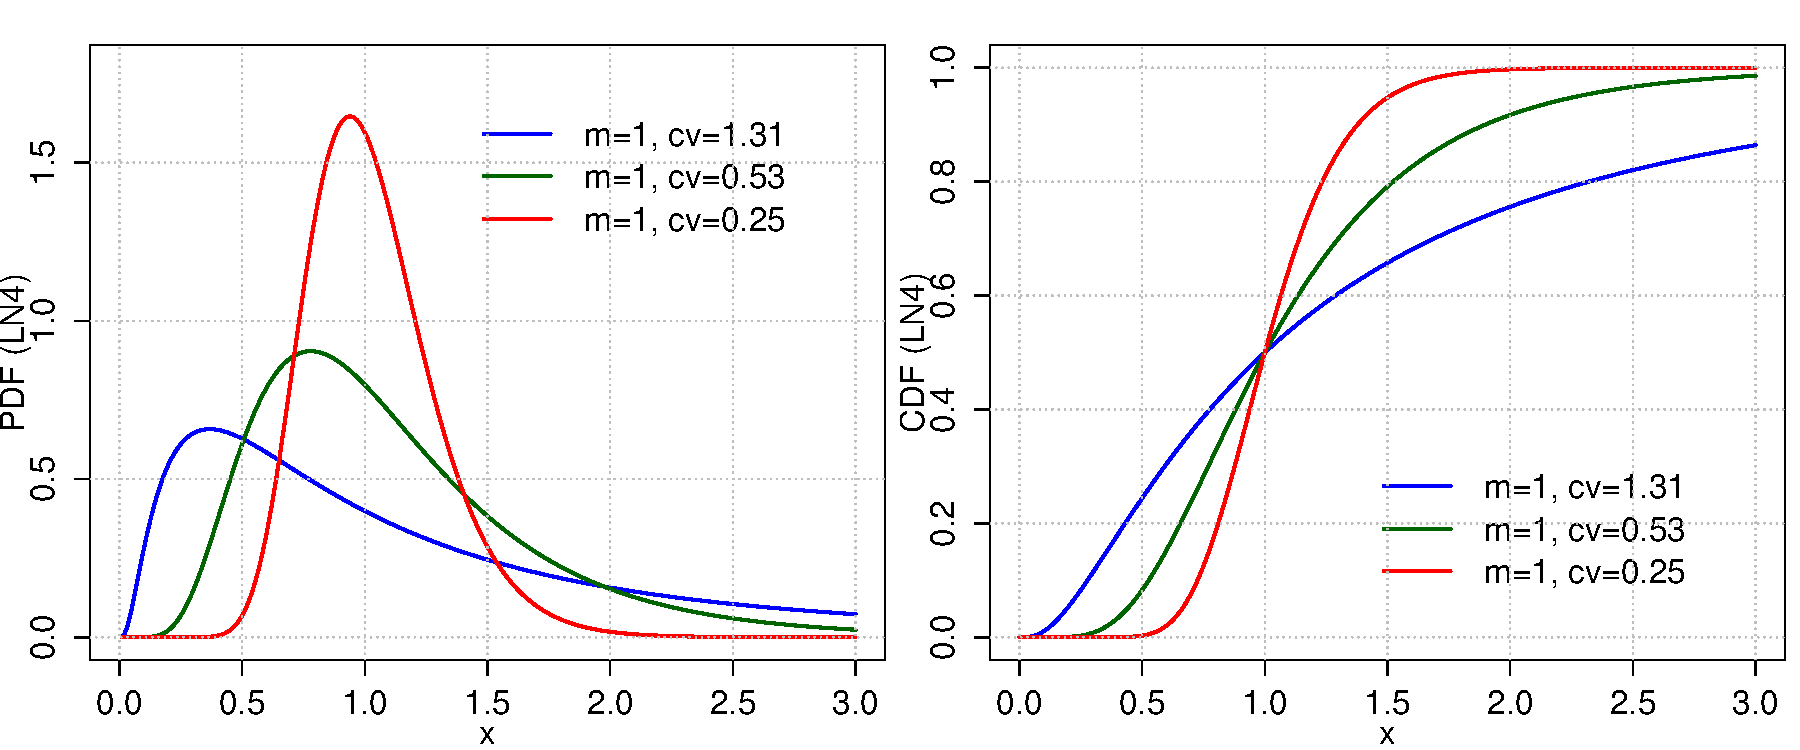
\includegraphics[width=140mm]{pics/LogNormal4.pdf}
 \caption{LogNormal4 distribution plotted using the provided R code.}
 \label{fig:LogNormal4}
\end{figure}

\subsubsection*{Parameter: median}

\noindent\begin{tabular}{p{2cm}cl}
\textbf{name} & & median / geometric mean \\
\textbf{type} & & scalar \\
\textbf{symbol} & & $m$  \\
\textbf{definition} & & $m>0$
\end{tabular}
\subsubsection*{Parameter: coefVar}

\noindent\begin{tabular}{p{2cm}cl}
\textbf{name} & & coefficient of variation \\
\textbf{type} & & scalar \\
\textbf{symbol} & & $cv$  \\
\textbf{definition} & & $cv>0$
\end{tabular}
\subsubsection*{Functions}

\smallskip \noindent \hspace{.2cm} \textbf{PDF} 
\begin{equation*}\frac{1}{x\sqrt{\ln(cv^2+1)}\sqrt{2\pi}}\ e^{-\frac{\left[\ln (x/m)\right]^2}{2\ln(cv^2+1)}}\end{equation*}
\smallskip \noindent \hspace{.2cm} \textbf{PDF in R}  
\begin{verbatim}1/(x*sqrt(log(cv^2+1))*sqrt(2*pi)) * exp( -(log(x/m))^2 / (2*log(cv^2+1)) )\end{verbatim}
\smallskip \noindent \hspace{.2cm} \textbf{CDF} 
\begin{equation*}\frac12 + \frac12\,\text{erf}\Big[\frac{\ln x-\ln m}{\sqrt{2}\sqrt{\log(cv^2+1)}}\Big]\end{equation*}
\smallskip \noindent \hspace{.2cm} \textbf{CDF in R} 
\begin{verbatim}1/2 + 1/2 * erf( (log(x)-log(m)) / (sqrt(2*log(cv^2+1))) )\end{verbatim}
\smallskip
\subsubsection*{Characteristics}
\smallskip
\section*{LogNormal5} 

  \bigskip 

\begin{tabular}{p{2cm}cl}
\textbf{name} & & Log-Normal 5 (ID: 0000004)\\ 
 
\textbf{type} & & continuous \\ 

\textbf{variate} & & $x$, scalar \\ 

\textbf{support} & & $x \in (0,+\infty)$
\end{tabular}

\begin{figure}[ht!]
\centering
  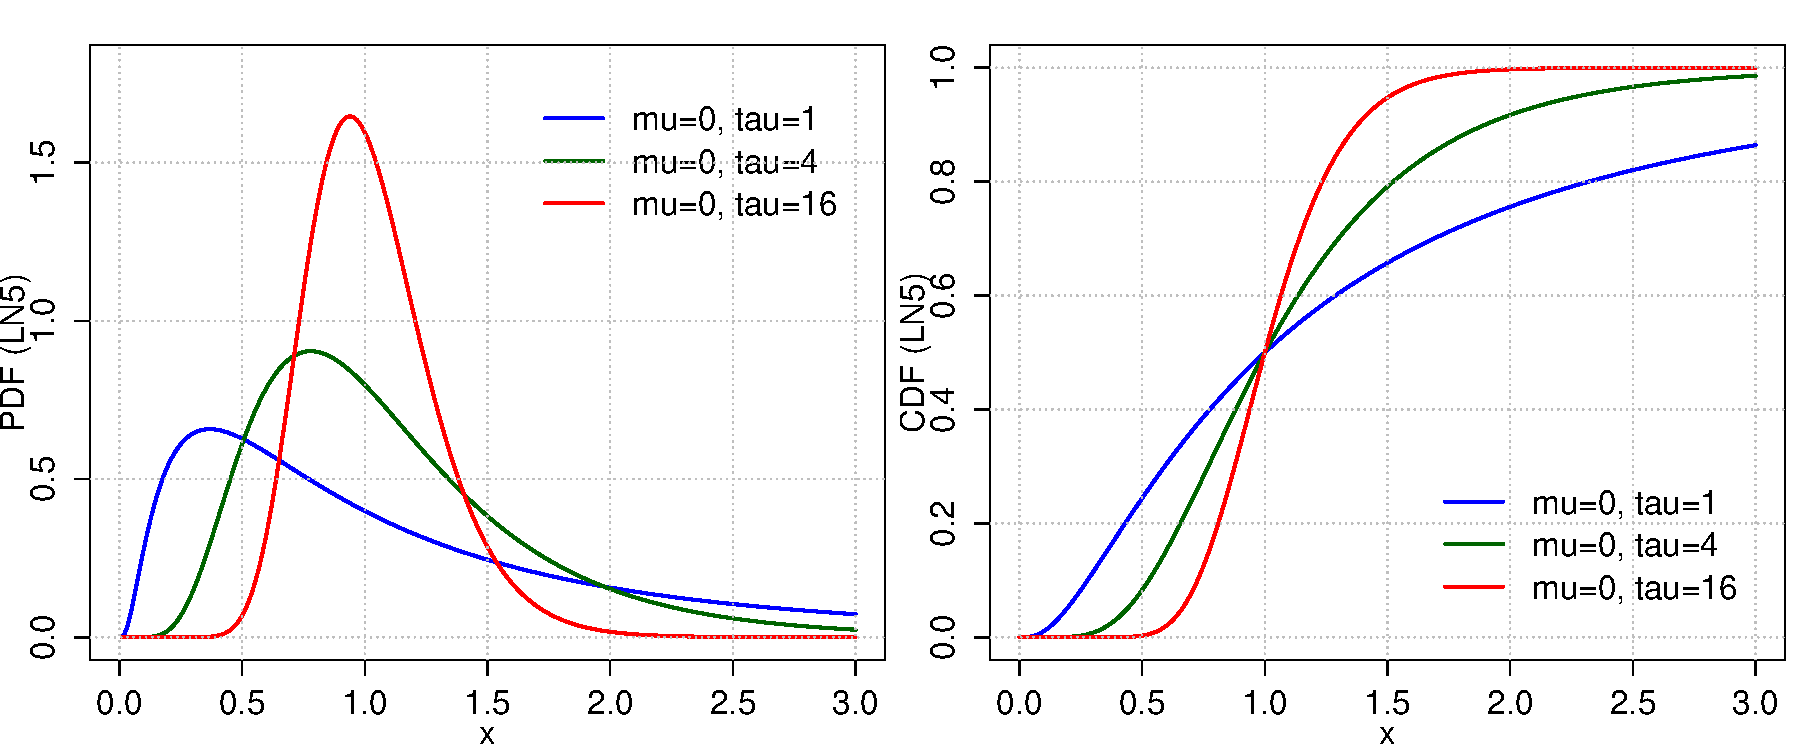
\includegraphics[width=140mm]{pics/LogNormal5.pdf}
 \caption{LogNormal5 distribution plotted using the provided R code.}
 \label{fig:LogNormal5}
\end{figure}

\subsubsection*{Parameter: meanLog}

\noindent\begin{tabular}{p{2cm}cl}
\textbf{name} & & mean of log(x) \\
\textbf{type} & & scalar \\
\textbf{symbol} & & $\mu$  \\
\textbf{definition} & & $\mu \in R$
\end{tabular}
\subsubsection*{Parameter: precision}

\noindent\begin{tabular}{p{2cm}cl}
\textbf{name} & & precision \\
\textbf{type} & & scalar \\
\textbf{symbol} & & $\tau$  \\
\textbf{definition} & & $\tau > 0$
\end{tabular}
\subsubsection*{Functions}

\smallskip \noindent \hspace{.2cm} \textbf{PDF} 
\begin{equation*}\sqrt{\frac{\tau}{2 \pi}} \frac{1}{x}e^{-\frac{\tau}{2}(\log x-\mu)^2}\end{equation*}
\smallskip \noindent \hspace{.2cm} \textbf{PDF in R}  
\begin{verbatim}sqrt(tau / (2*pi)) * (1/x) * exp(- (tau/2)*(log(x)-mu)^2 )\end{verbatim}
\smallskip \noindent \hspace{.2cm} \textbf{CDF} 
\begin{equation*}\frac12 + \frac12\,\text{erf}\Big[\frac{\ln x-\mu}{\sqrt{2/\tau}}\Big]\end{equation*}
\smallskip \noindent \hspace{.2cm} \textbf{CDF in R} 
\begin{verbatim}1/2 + 1/2 * erf( (log(x)-mu) / sqrt(2/tau) )\end{verbatim}
\smallskip
\subsubsection*{Characteristics}
\smallskip
%\section*{LogNormal6} 
%
%  \bigskip 
%
%\begin{tabular}{p{2cm}cl}
%\textbf{name} & & Log-Normal 6 (ID: 0000019)\\ 
% 
%\textbf{type} & &  \\ 
%
%\textbf{variate} & & $$,  \\ 
%
%\textbf{support} & & $$
%\end{tabular}
%
%\begin{figure}[ht!]
%\centering
%  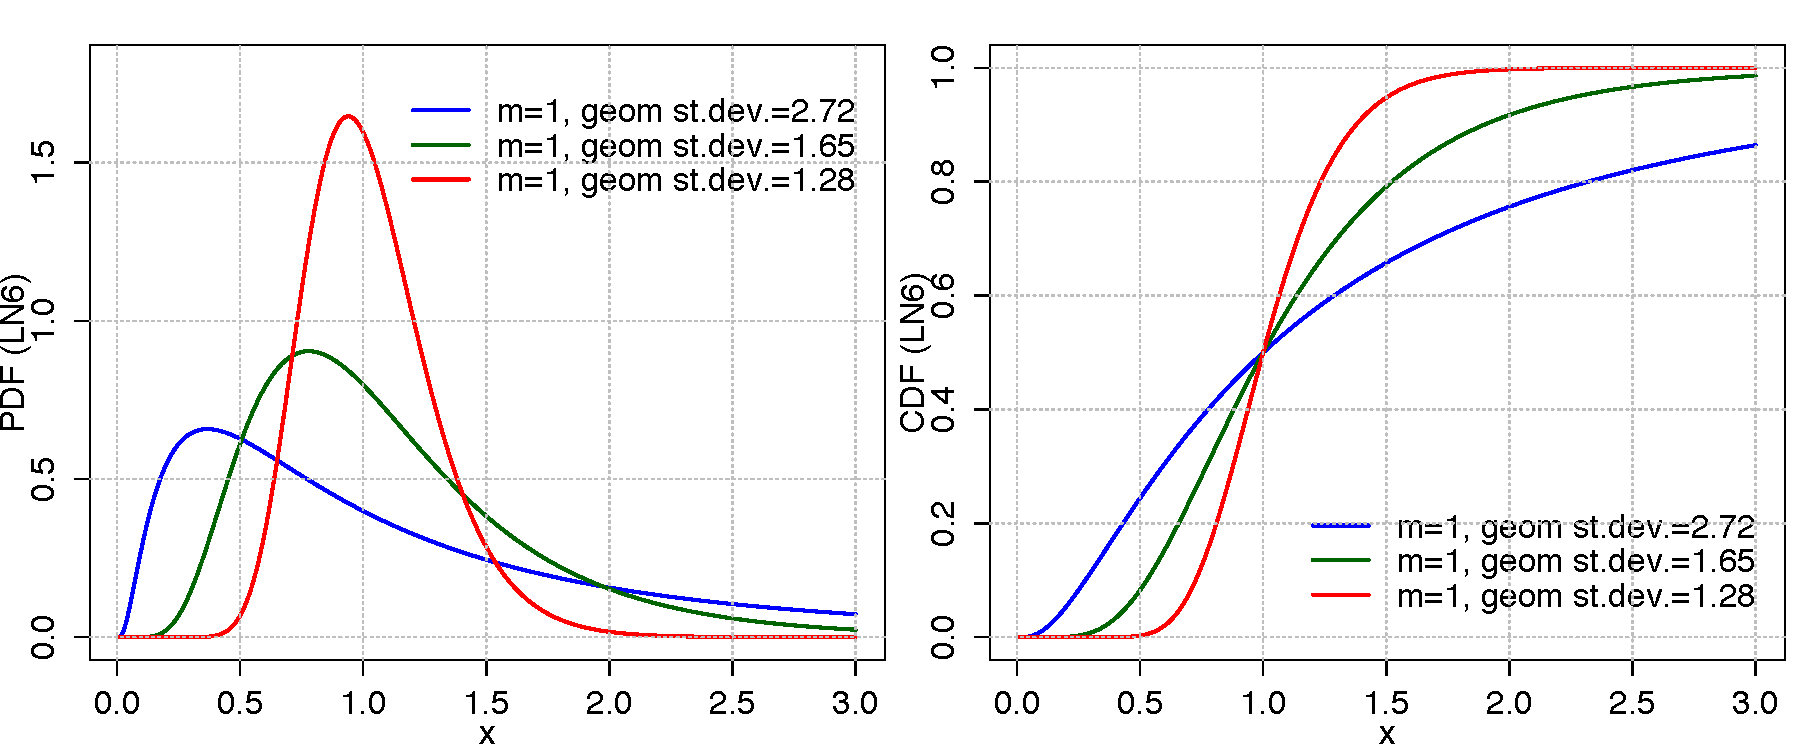
\includegraphics[width=140mm]{pics/LogNormal6.pdf}
% \caption{LogNormal6 distribution plotted using the provided R code.}
% \label{fig:LogNormal6}
%\end{figure}
%
%\subsubsection*{Functions}
%
%\smallskip \noindent \hspace{.2cm} \textbf{} 
%\begin{equation*}\end{equation*}
%\smallskip \noindent \hspace{.2cm} \textbf{CDF} 
%\begin{equation*}\end{equation*}
%\smallskip
%\subsubsection*{Characteristics}
%\smallskip
\section*{LogUniform1} 

  \bigskip 

\begin{tabular}{p{2cm}cl}
\textbf{name} & & Log-Uniform (ID: 0000044)\\ 
 
\textbf{type} & & continuous \\ 

\textbf{variate} & & $x$, scalar \\ 

\textbf{support} & & $x \in (min,max)$
\end{tabular}

\begin{figure}[ht!]
\centering
  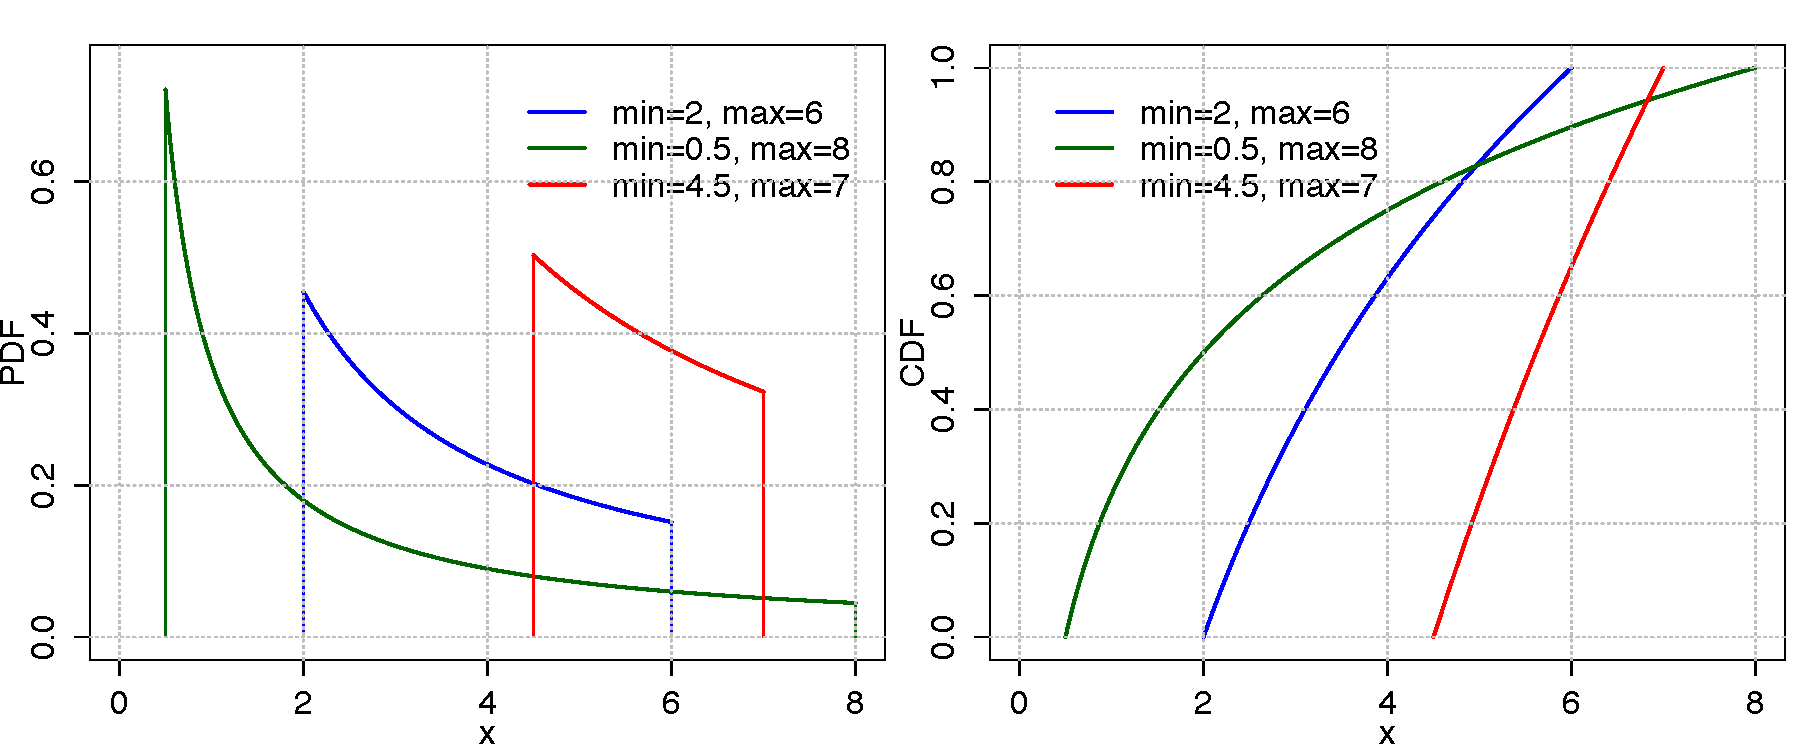
\includegraphics[width=140mm]{pics/LogUniform.pdf}
 \caption{LogUniform distribution plotted using the provided R code.}
 \label{fig:LogUniform}
\end{figure}

\subsubsection*{Parameter: minimum}

\noindent\begin{tabular}{p{2cm}cl}
\textbf{name} & & minimum \\
\textbf{type} & & scalar \\
\textbf{symbol} & & $min$  \\
\textbf{definition} & & $min>0$
\end{tabular}
\subsubsection*{Parameter: maximum}

\noindent\begin{tabular}{p{2cm}cl}
\textbf{name} & & maximum \\
\textbf{type} & & scalar \\
\textbf{symbol} & & $max$  \\
\textbf{definition} & & $max \geq min$
\end{tabular}
\subsubsection*{Functions}

\smallskip \noindent \hspace{.2cm} \textbf{PDF} 
\begin{equation*}\frac{1}{x(\log(max) - \log(min))}\end{equation*}
\smallskip \noindent \hspace{.2cm} \textbf{PDF in R}  
\begin{verbatim}1/(x*(log(max) - log(min)))\end{verbatim}
\smallskip \noindent \hspace{.2cm} \textbf{CDF} 
\begin{equation*}\frac{\log(x) - \log(min)}{\log(max) - \log(min)}\end{equation*}
\smallskip \noindent \hspace{.2cm} \textbf{CDF in R} 
\begin{verbatim}(log(x) - log(min)) / (log(max) - log(min))\end{verbatim}
\smallskip
\subsubsection*{Characteristics}
\smallskip
\section*{MixtureDistribution1} 

  \bigskip 

\begin{tabular}{p{2cm}cl}
\textbf{name} & & Mixture Distribution (ID: 0000053)\\ 
 
\textbf{variate} & & $-$ \\ 

\textbf{support} & & $-$
\end{tabular}

%\begin{figure}[ht!]
%\centering
%  \includegraphics[width=140mm]{pics/MixtureDistribution.pdf}
% \caption{MixtureDistribution distribution plotted using the provided R code.}
% \label{fig:MixtureDistribution}
%\end{figure}
\begin{figure}[htb!]
\centering
  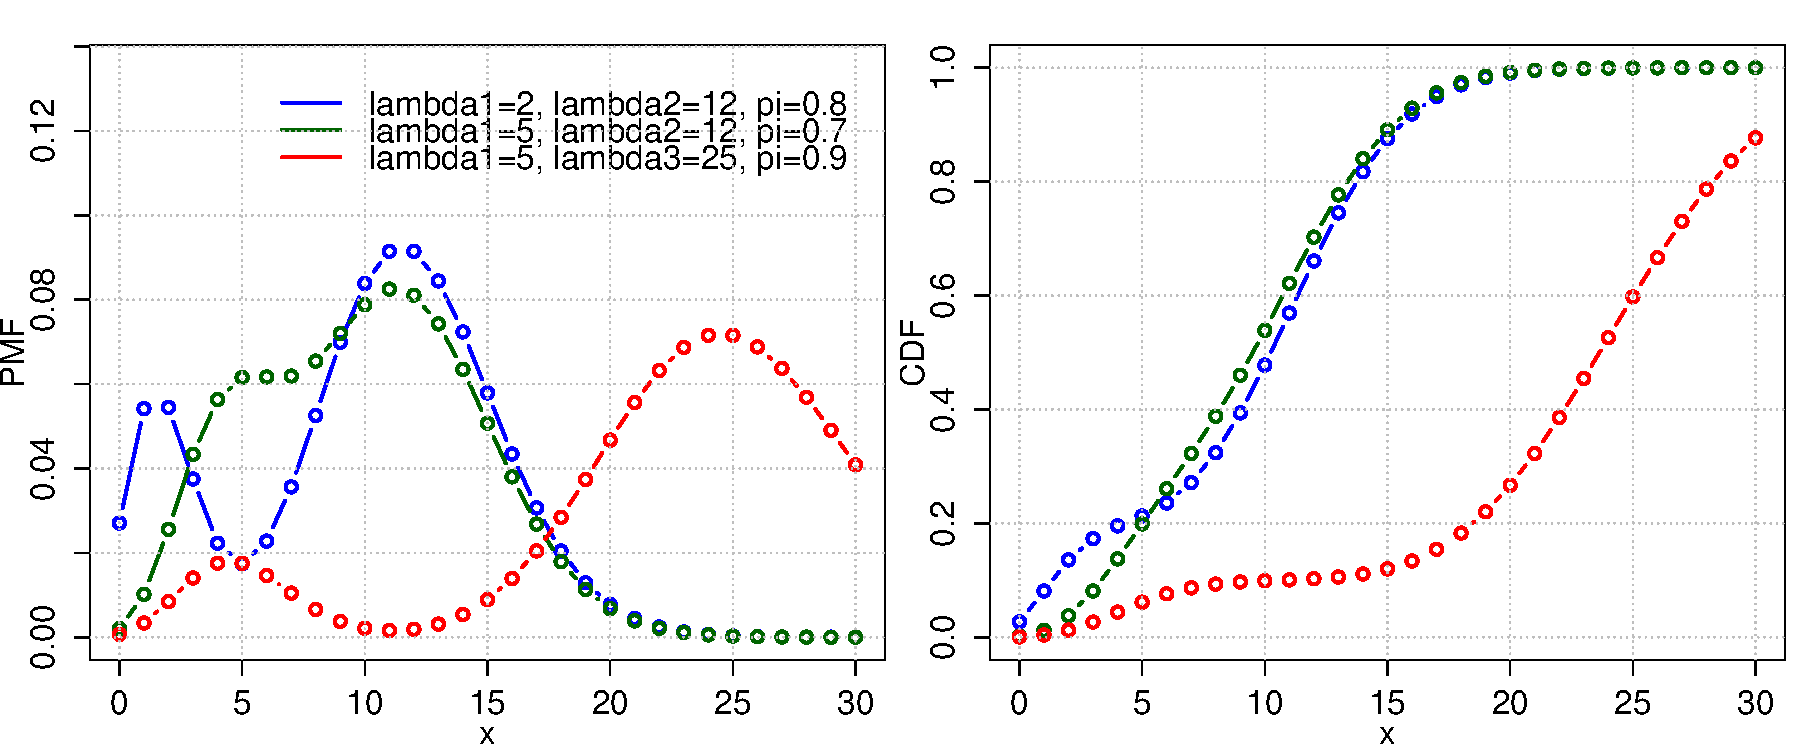
\includegraphics[width=140mm]{pics/MixturePoisson.pdf}
 \caption{Example 1: PMF and CDF of the Mixture Poisson distribution plotted using the formula for 
 for various values as shown in the legend of the left plot. The PMF reads: $(1\!-\!\pi_1) \,\lambda_1^k/k! \,\exp(-\lambda_1) + \pi_1\,\lambda_2^k / k! \, \exp(-\lambda_2)$. The CDF reads: $(1-\pi_1)\,\Gamma(\lfloor k+1 , \lambda_1 \rfloor) / \lfloor k \rfloor!+\pi_1 \,\Gamma(\lfloor k+1 , \lambda_2 \rfloor) / \lfloor k \rfloor!$.}
 \label{fig:MixturePoisson_pmf_cdf}
\end{figure}
\begin{figure}[htb!]
\centering
  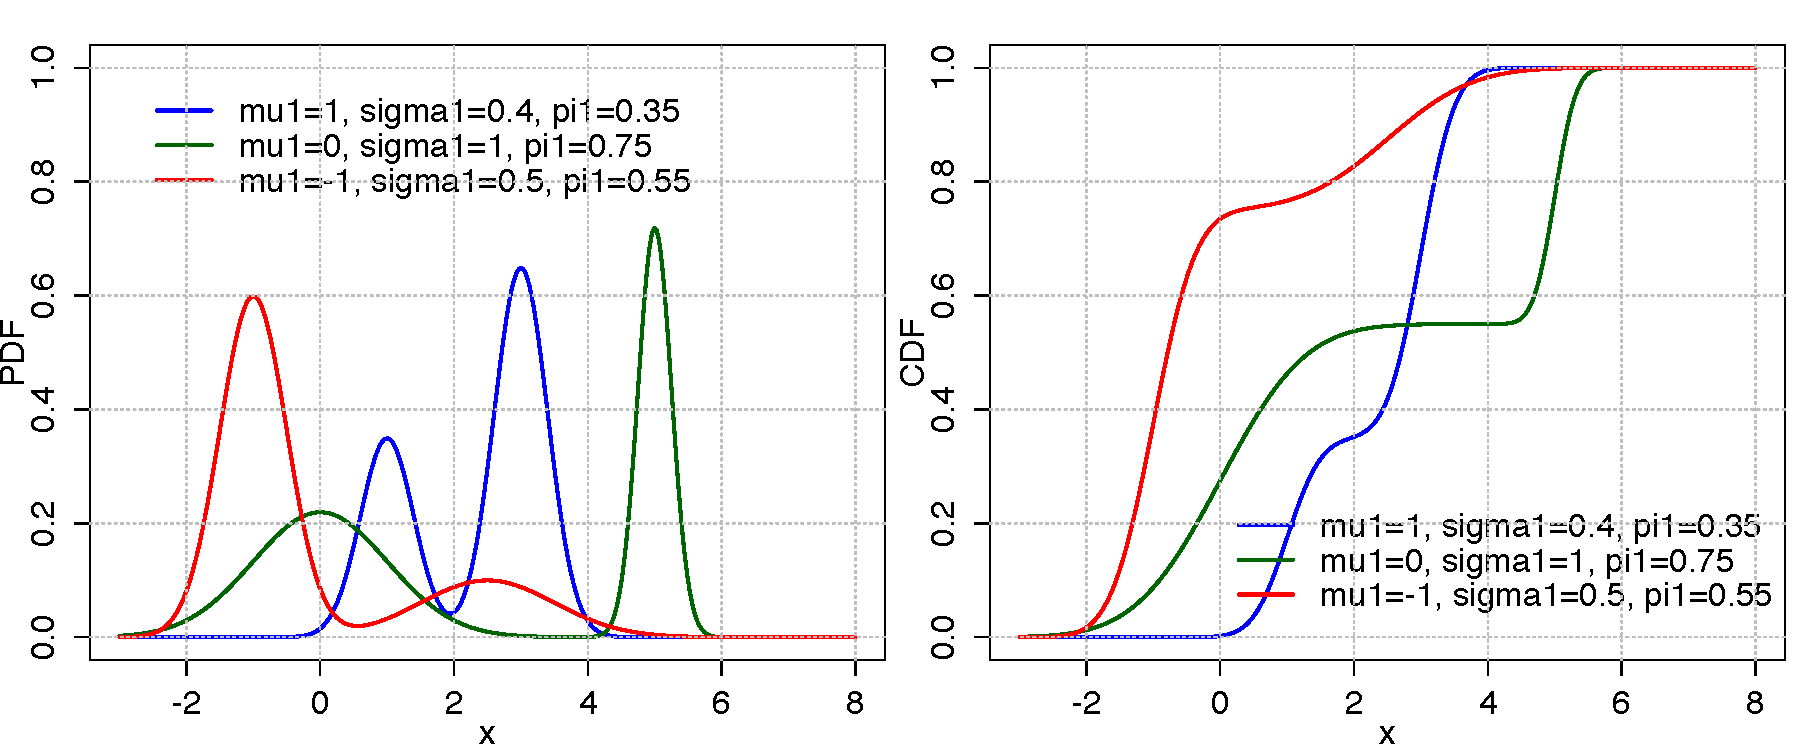
\includegraphics[width=140mm]{pics/MixtureNormal.pdf}
 \caption{Example 2: PDF and CDF of the Mixture Normal distribution plotted using the formula for 
 for various values as shown in the legend of the left plot. The PDF reads: $(1\!-\!\pi_1)\times1/(\sigma_1\sqrt{2\pi})\exp(-(x-\mu_1)^2/(2\sigma_1^2)) + \pi_1\,\times1/(\sigma_2\sqrt{2\pi})\exp(-(x-\mu_2)^2/(2\sigma_2^2))$. The CDF reads: $(1\!-\!\pi_1)\times1/2 (1 + erf((x-\mu_1)/(\sigma_1\sqrt{2})))  + \pi_1\,\times1/2  (1 + erf((x-\mu_2)/(\sigma_2\sqrt{2})))$.}
 \label{fig:MixtureNormal_pdf_cdf}
\end{figure}

\subsubsection*{Parameter: weight}

\noindent\begin{tabular}{p{2cm}cl}
\textbf{name} & & mixing coefficients \\
\textbf{type} & & vector \\
\textbf{symbol} & & $\pi_1, \ldots, \pi_k$  \\
\textbf{definition} & & $\Sigma_{i=1}^K \pi_i=1; 0\le \pi_i \le 1$
\end{tabular}
\subsubsection*{Functions}

\smallskip \noindent \hspace{.2cm} \textbf{PDF} 
\begin{equation*}f(x; \pi, \theta) = \sum_{i=1}^{K} \pi_{i}\; p_i(x; \theta_i) \text{ where } p_i(x; \theta_i) \text{ the PDF of the } i^{th} \text{ component with parameters } \theta_i\end{equation*}
\smallskip \noindent \hspace{.2cm} \textbf{PMF} 
\begin{equation*}f(x; \pi, \theta) = \sum_{i=1}^{K} \pi_{i}\; p_i(x; \theta_i) \text{ where } p_i(x; \theta_i) \text{ the PMF of the } i^{th} \text{ component with parameters } \theta_i\end{equation*}
\smallskip
\subsubsection*{Characteristics}
\smallskip
\section*{Multinomial1} 

  \bigskip 

\begin{tabular}{p{2cm}cl}
\textbf{name} & & Multinomial (ID: 0000062)\\ 
 
\textbf{type} & & discrete \\ 

\textbf{variate} & & $X$, vector \\ 

\textbf{support} & & $X_i \in \{0,\dots,n\}, \Sigma X_i = n$
\end{tabular}

%\begin{figure}[ht!]
%\centering
%  \includegraphics[width=140mm]{pics/Multinomial.pdf}
% \caption{Multinomial distribution plotted using the provided R code.}
% \label{fig:Multinomial}
%\end{figure}

\subsubsection*{Parameter: numberOfTrials}

\noindent\begin{tabular}{p{2cm}cl}
\textbf{name} & & number of trials \\
\textbf{type} & & scalar \\
\textbf{symbol} & & $n$  \\
\textbf{definition} & & $n > 0, n \in N$
\end{tabular}
\subsubsection*{Parameter: probabilityOfSuccess}

\noindent\begin{tabular}{p{2cm}cl}
\textbf{name} & & event probabilities \\
\textbf{type} & & vector \\
\textbf{symbol} & & $p_1, \ldots, p_k$  \\
\textbf{definition} & & $p_1, \ldots, p_k, \Sigma p_i = 1$
\end{tabular}
\subsubsection*{Functions}

\smallskip \noindent \hspace{.2cm} \textbf{PMF} 
\begin{equation*}\frac{n!}{x_1!\cdots x_k!} p_1^{x_1} \cdots p_k^{x_k}\end{equation*}
\smallskip \noindent \hspace{.2cm} \textbf{CDF} 
\begin{equation*}-\end{equation*}
\smallskip
\subsubsection*{Characteristics}
\smallskip \noindent \hspace{.2cm} \textbf{Mean} 
\begin{equation*}E\{X_i\} = np_i\end{equation*}
\smallskip \noindent \hspace{.2cm} \textbf{Variance} 
\begin{align*}Var(X_i) &= n p_i (1-p_i) \\
Cov(X_i,X_j) &= - n p_i p_j~~(i\neq j)\end{align*}
\smallskip
\section*{MultivariateNormal1} 

  \bigskip 

\begin{tabular}{p{2cm}cl}
\textbf{name} & & Multivariate Normal 1 (ID: 0000072)\\ 
 
\textbf{type} & & continuous \\ 

\textbf{variate} & & $x$, vector \\ 

\textbf{support} & & $x \in \mu + \text{span}(\Sigma) \subseteq  R^k$
\end{tabular}

%\begin{figure}[ht!]
%\centering
%  \includegraphics[width=140mm]{pics/MultivariateNormal1.pdf}
% \caption{MultivariateNormal1 distribution plotted using the provided R code.}
% \label{fig:MultivariateNormal1}
%\end{figure}

\subsubsection*{Parameter: mean}

\noindent\begin{tabular}{p{2cm}cl}
\textbf{name} & & location \\
\textbf{type} & & vector \\
\textbf{symbol} & & $\mu$  \\
\textbf{definition} & & $\mu \in R^k$
\end{tabular}
\subsubsection*{Parameter: covarianceMatrix}

\noindent\begin{tabular}{p{2cm}cl}
\textbf{name} & & covariance matrix \\
\textbf{type} & & matrix \\
\textbf{symbol} & & $\Sigma$  \\
\textbf{definition} & & $\Sigma \in R^{k\times k}$
\end{tabular}
\subsubsection*{Functions}

\smallskip \noindent \hspace{.2cm} \textbf{PDF} 
\begin{equation*}(2\pi)^{-\frac{k}{2}}|\Sigma|^{-\frac{1}{2}}\, e^{ -\frac{1}{2}(x-\mu)'\Sigma^{-1}(x-\mu) }\end{equation*}
\smallskip \noindent \hspace{.2cm} \textbf{CDF} 
\begin{equation*}\text{no analytic expression}\end{equation*}
\smallskip
\subsubsection*{Characteristics}
\smallskip \noindent \hspace{.2cm} \textbf{Mean} 
\begin{equation*}\mu\end{equation*}
\smallskip \noindent \hspace{.2cm} \textbf{Mode} 
\begin{equation*}\mu\end{equation*}
\smallskip \noindent \hspace{.2cm} \textbf{Variance} 
\begin{equation*}\Sigma\end{equation*}
\smallskip
\section*{MultivariateNormal2} 

  \bigskip 

\begin{tabular}{p{2cm}cl}
\textbf{name} & & Multivariate Normal 2 (ID: 0000081)\\ 
 
\textbf{type} & & continuous \\ 

\textbf{variate} & & $x$, vector \\ 

\textbf{support} & & $x \in \mu + \text{span}(\Sigma) \subseteq  R^k$
\end{tabular}

%\begin{figure}[ht!]
%\centering
%  \includegraphics[width=140mm]{pics/MultivariateNormal2.pdf}
% \caption{MultivariateNormal2 distribution plotted using the provided R code.}
% \label{fig:MultivariateNormal2}
%\end{figure}

\subsubsection*{Parameter: mean}

\noindent\begin{tabular}{p{2cm}cl}
\textbf{name} & & location \\
\textbf{type} & & vector \\
\textbf{symbol} & & $\mu$  \\
\textbf{definition} & & $\mu \in R^k$
\end{tabular}
\subsubsection*{Parameter: precisionMatrix}

\noindent\begin{tabular}{p{2cm}cl}
\textbf{name} & & precision matrix \\
\textbf{type} & & matrix \\
\textbf{symbol} & & $T$  \\
\textbf{definition} & & $-$
\end{tabular}
\subsubsection*{Functions}

\smallskip \noindent \hspace{.2cm} \textbf{PDF} 
\begin{equation*}(2\pi)^{-d/2}|T|^{\frac{1}{2}}\, \exp\big( -\frac{1}{2}(x-\mu)' T (x-\mu) \big)\end{equation*}
\smallskip \noindent \hspace{.2cm} \textbf{CDF} 
\begin{equation*}\text{no analytic expression}\end{equation*}
\smallskip
\subsubsection*{Characteristics}
\smallskip \noindent \hspace{.2cm} \textbf{Mean} 
\begin{equation*}\mu\end{equation*}
\smallskip \noindent \hspace{.2cm} \textbf{Mode} 
\begin{equation*}\mu\end{equation*}
\smallskip \noindent \hspace{.2cm} \textbf{Variance} 
\begin{equation*}\Sigma\end{equation*}
\smallskip
\section*{MultivariateStudentT1} 

  \bigskip 

\begin{tabular}{p{2cm}cl}
\textbf{name} & & Multivariate (Student) T 1 (ID: 0000088)\\ 
 
\textbf{type} & & continuous \\ 

\textbf{variate} & & $x$, vector \\ 

\textbf{support} & & $x \in R^p$
\end{tabular}

%\begin{figure}[ht!]
%\centering
%  \includegraphics[width=140mm]{pics/MultivariateStudentT1.pdf}
% \caption{MultivariateStudentT1 distribution plotted using the provided R code.}
% \label{fig:MultivariateStudentT1}
%\end{figure}

\subsubsection*{Parameter: mean}

\noindent\begin{tabular}{p{2cm}cl}
\textbf{name} & & location \\
\textbf{type} & & vector \\
\textbf{symbol} & & $\mu$  \\
\textbf{definition} & & $\mu = [\mu_1, \dots, \mu_p]^T, \mu_i \in R$
\end{tabular}
\subsubsection*{Parameter: covarianceMatrix}

\noindent\begin{tabular}{p{2cm}cl}
\textbf{name} & & covariance matrix \\
\textbf{type} & & matrix \\
\textbf{symbol} & & $\Sigma$  \\
\textbf{definition} & & $\Sigma, \text{ positive-definite real } p\times p \text{ matrix}$
\end{tabular}
\subsubsection*{Parameter: degreesOfFreedom}

\noindent\begin{tabular}{p{2cm}cl}
\textbf{name} & & degrees of freedom \\
\textbf{type} & & scalar \\
\textbf{symbol} & & $\nu$  \\
\textbf{definition} & & $\nu$
\end{tabular}
\subsubsection*{Functions}

\smallskip \noindent \hspace{.2cm} \textbf{PDF} 
\begin{equation*}\frac{\Gamma\left[(\nu+p)/2\right]}{\Gamma(\nu/2)\nu^{p/2}\pi^{p/2}\left|\Sigma\right|^{1/2}\left[1+\frac{1}{\nu}(x-\mu)^{\rm T}\Sigma^{-1}(x-\mu)\right]^{(\nu+p)/2}}\end{equation*}
\smallskip \noindent \hspace{.2cm} \textbf{CDF} 
\begin{equation*}\text{no analytic expression}\end{equation*}
\smallskip
\subsubsection*{Characteristics}
\smallskip \noindent \hspace{.2cm} \textbf{Mean} 
\begin{equation*}\begin{cases}
\mu & \text{for }\nu > 1 \\
undefined & \text{else} 
\end{cases}\end{equation*}
\smallskip \noindent \hspace{.2cm} \textbf{Median} 
\begin{equation*}\mu\end{equation*}
\smallskip \noindent \hspace{.2cm} \textbf{Mode} 
\begin{equation*}\mu\end{equation*}
\smallskip \noindent \hspace{.2cm} \textbf{Variance} 
\begin{equation*}\begin{cases}
\frac{\nu}{\nu-2} \Sigma & \text{for }\nu > 2 \\
undefined & \text{else} 
\end{cases}\end{equation*}
\smallskip
\section*{MultivariateStudentT2} 

  \bigskip 

\begin{tabular}{p{2cm}cl}
\textbf{name} & & Multivariate (Student) T 2 (ID: 0000098)\\ 
 
\textbf{type} & & continuous \\ 

\textbf{variate} & & $x$, vector \\ 

\textbf{support} & & $x \in R^p, k\geq 2$
\end{tabular}

%\begin{figure}[ht!]
%\centering
%  \includegraphics[width=140mm]{pics/MultivariateStudentT2.pdf}
% \caption{MultivariateStudentT2 distribution plotted using the provided R code.}
% \label{fig:MultivariateStudentT2}
%\end{figure}

\subsubsection*{Parameter: mean}

\noindent\begin{tabular}{p{2cm}cl}
\textbf{name} & & location \\
\textbf{type} & & vector \\
\textbf{symbol} & & $\mu$  \\
\textbf{definition} & & $\mu = [\mu_1, \dots, \mu_p]^T, \mu_i \in R$
\end{tabular}
\subsubsection*{Parameter: precisionMatrix}

\noindent\begin{tabular}{p{2cm}cl}
\textbf{name} & & precision matrix \\
\textbf{type} & & matrix \\
\textbf{symbol} & & $T$  \\
\textbf{definition} & & $-$
\end{tabular}
\subsubsection*{Parameter: degreesOfFreedom}

\noindent\begin{tabular}{p{2cm}cl}
\textbf{name} & & degrees of freedom \\
\textbf{type} & & scalar \\
\textbf{symbol} & & $k$  \\
\textbf{definition} & & $-$
\end{tabular}
\subsubsection*{Functions}

\smallskip \noindent \hspace{.2cm} \textbf{PDF} 
\begin{equation*}\frac{\Gamma((k+d)/2)}{\Gamma(k/2) k^{d/2} \pi^{d/2}}|T|^{1/2} \Big[ 1 + \frac{1}{k}(x-\mu)' T (x-\mu) \Big]^{-(k+d)/2}\end{equation*}
\smallskip \noindent \hspace{.2cm} \textbf{CDF} 
\begin{equation*}-\end{equation*}
\smallskip
\subsubsection*{Characteristics}
\smallskip
\section*{Nakagami1} 

  \bigskip 

\begin{tabular}{p{2cm}cl}
\textbf{name} & & Nakagami (ID: 0000108)\\ 
 
\textbf{type} & & continuous \\ 

\textbf{variate} & & $x$, scalar \\ 

\textbf{support} & & $x \in (0,+\infty)$
\end{tabular}

\begin{figure}[ht!]
\centering
  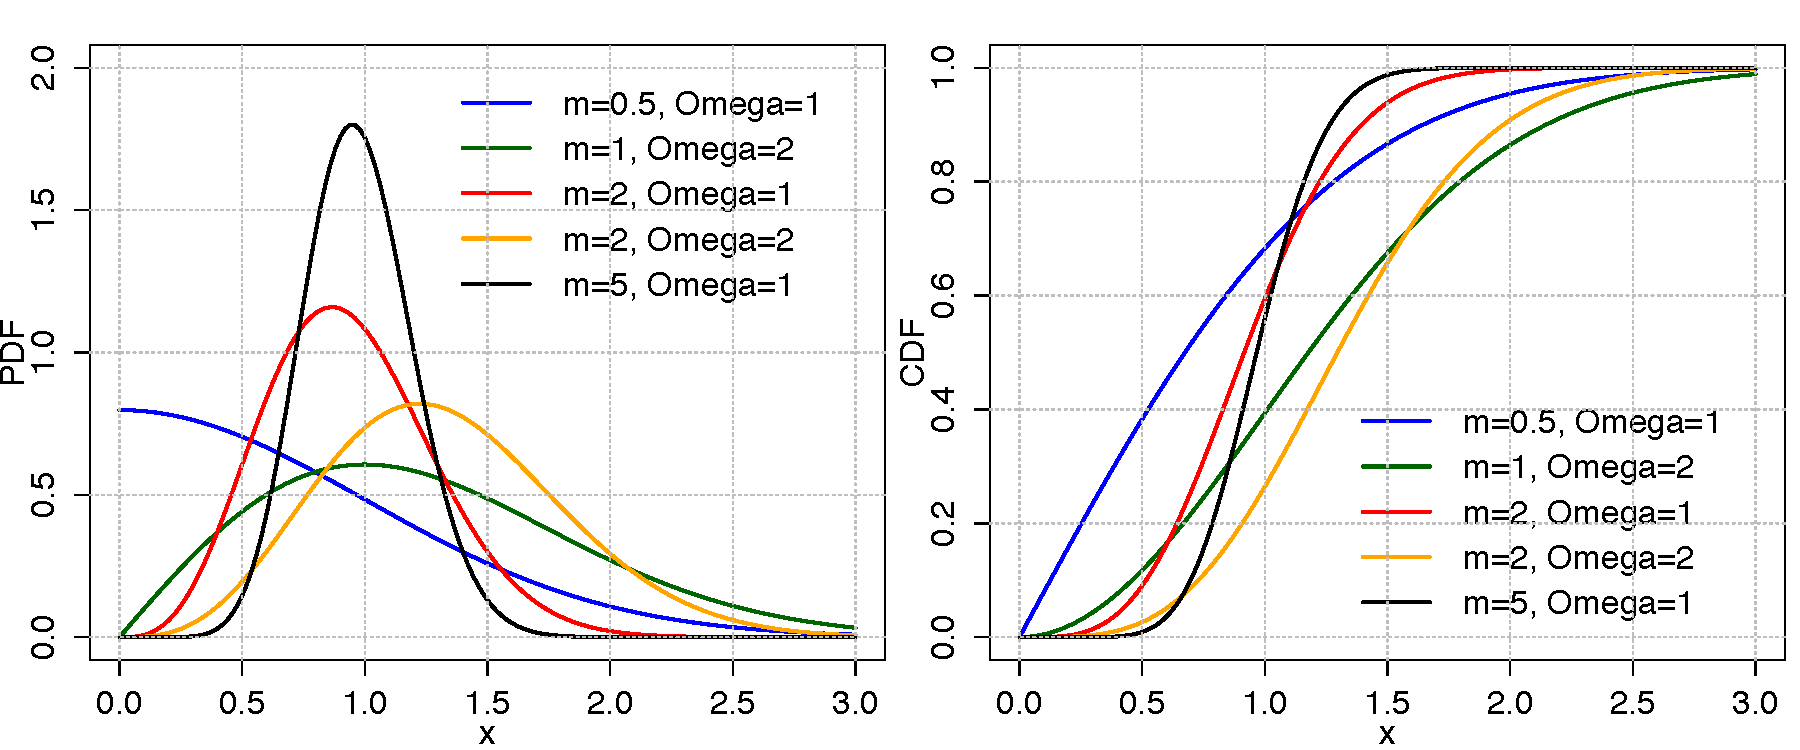
\includegraphics[width=140mm]{pics/Nakagami.pdf}
 \caption{Nakagami distribution plotted using the provided R code.}
 \label{fig:Nakagami}
\end{figure}

\subsubsection*{Parameter: shape}

\noindent\begin{tabular}{p{2cm}cl}
\textbf{name} & & shape \\
\textbf{type} & & scalar \\
\textbf{symbol} & & $m$  \\
\textbf{definition} & & $m > 0$
\end{tabular}
\subsubsection*{Parameter: spread}

\noindent\begin{tabular}{p{2cm}cl}
\textbf{name} & & spread \\
\textbf{type} & & scalar \\
\textbf{symbol} & & $\Omega$  \\
\textbf{definition} & & $ \Omega > 0$
\end{tabular}
\subsubsection*{Functions}

\smallskip \noindent \hspace{.2cm} \textbf{PDF} 
\begin{equation*}\frac{2m^m}{\Gamma(m)\Omega^m}x^{2m-1} \exp(-\frac{m}{\omega}x^2)\end{equation*}
\smallskip \noindent \hspace{.2cm} \textbf{PDF in R}  
\begin{verbatim}2*m^m / (gamma(m)*Omega^m)*x^(2*m-1)*exp(-m/Omega*x^2)\end{verbatim}
\smallskip \noindent \hspace{.2cm} \textbf{CDF} 
\begin{equation*}\frac{\gamma(m,\frac{m}{\Omega}x^2)}{\Gamma(m)}\end{equation*}
\smallskip \noindent \hspace{.2cm} \textbf{CDF in R} 
\begin{verbatim}Igamma(m,m/Omega*x^2,lower=T)/gamma(m)\end{verbatim}
\smallskip
\subsubsection*{Characteristics}
\smallskip \noindent \hspace{.2cm} \textbf{Mean} 
\begin{equation*}\frac{\Gamma(m+\frac{1}{2})}{\Gamma(m)} \Big(\frac{\Omega}{m}\Big)^{\frac12}\end{equation*}
\smallskip \noindent \hspace{.2cm} \textbf{Median} 
\begin{equation*}\sqrt{\Omega}\end{equation*}
\smallskip \noindent \hspace{.2cm} \textbf{Mode} 
\begin{equation*}\frac{\sqrt{2}}{2} \Big(\frac{(2m-1)\Omega}{m} \Big)^{1/2}\end{equation*}
\smallskip \noindent \hspace{.2cm} \textbf{Variance} 
\begin{equation*}\Omega \Big(1-\frac{1}{m}\Big(\frac{\Gamma(m+\frac{1}{2})}{\Gamma(m)}\Big)^2 \Big)\end{equation*}
\smallskip
\section*{NegativeBinomial1} 

  \bigskip 

\begin{tabular}{p{2cm}cl}
\textbf{name} & & Negative Binomial 1 (ID: 0000118)\\ 
 
\textbf{type} & & discrete \\ 

\textbf{variate} & & $k$, scalar \\ 

\textbf{support} & & $k \in \{0,1,2,3,\dots\}$ \text{ -- number of failures}
\end{tabular}

\begin{figure}[ht!]
\centering
  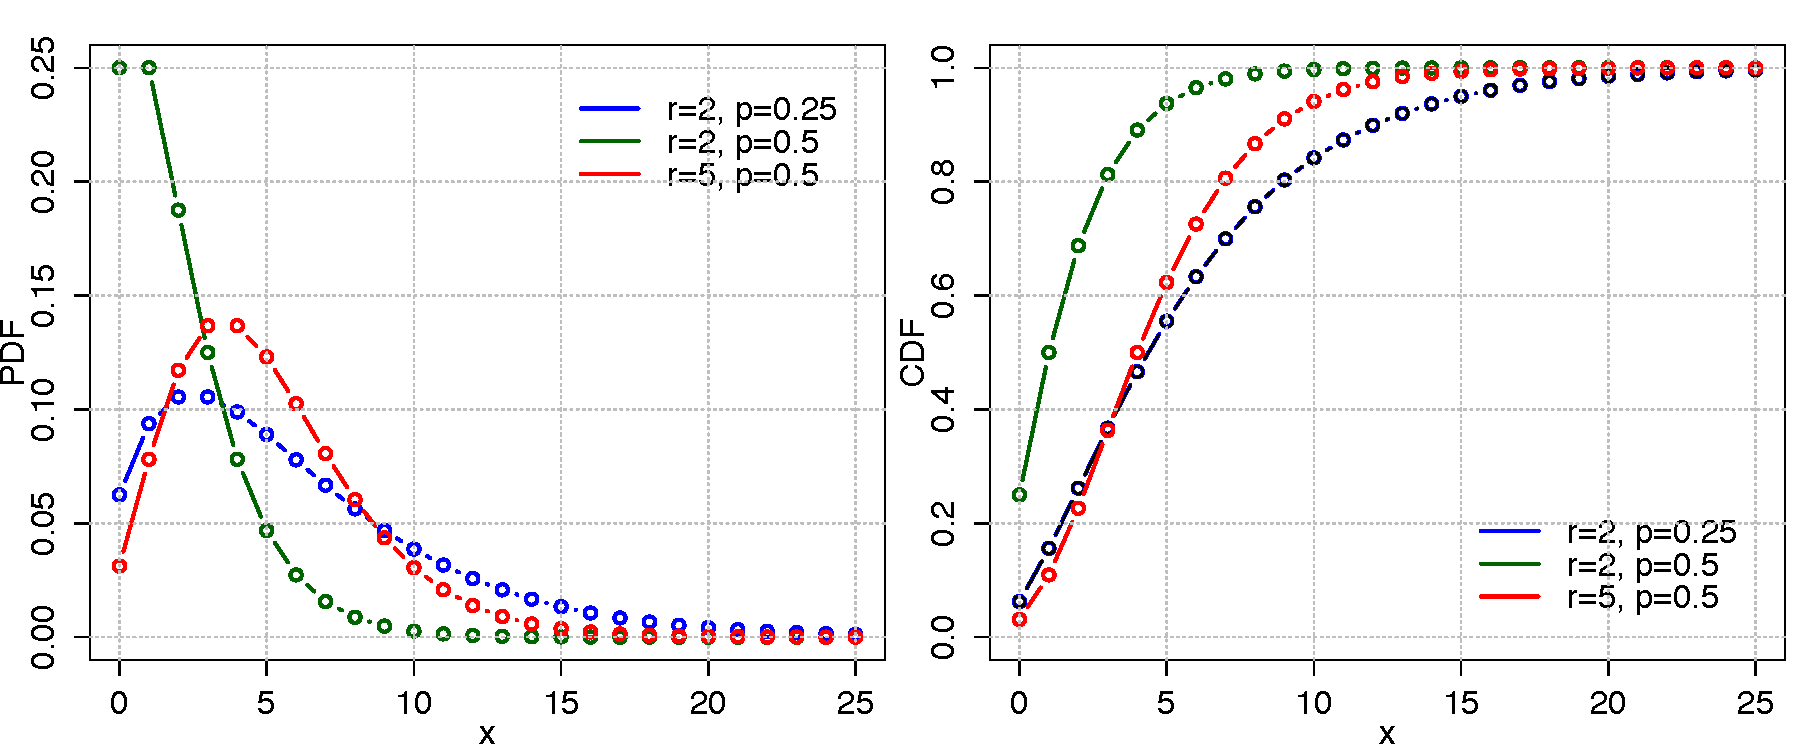
\includegraphics[width=140mm]{pics/NegativeBinomial1.pdf}
 \caption{NegativeBinomial1 distribution plotted using the provided R code.}
 \label{fig:NegativeBinomial1}
\end{figure}

\subsubsection*{Parameter: numberOfSuccesses}

\noindent\begin{tabular}{p{2cm}cl}
\textbf{name} & & number of successes \\
\textbf{type} & & scalar \\
\textbf{symbol} & & $r$  \\
\textbf{definition} & & $r > 0, r \in N$
\end{tabular}
\subsubsection*{Parameter: probability}

\noindent\begin{tabular}{p{2cm}cl}
\textbf{name} & & success probability \\
\textbf{type} & & scalar \\
\textbf{symbol} & & $p$  \\
\textbf{definition} & & $p \in (0,1)$
\end{tabular}
\subsubsection*{Functions}

\smallskip \noindent \hspace{.2cm} \textbf{PMF} 
\begin{equation*}\binom {k+r-1}k p^r (1-p)^k\end{equation*}
\smallskip \noindent \hspace{.2cm} \textbf{PMF in R}  
\begin{verbatim}choose(k+r-1,k)*p^r * (1-p)^k\end{verbatim}
\smallskip \noindent \hspace{.2cm} \textbf{CDF} 
\begin{equation*}1 - I_{p}(k+1, r)\end{equation*}
\smallskip \noindent \hspace{.2cm} \textbf{CDF in R} 
\begin{verbatim}1 - Rbeta(p, r, k+1,lower = F)\end{verbatim}
\smallskip
\subsubsection*{Characteristics}
\smallskip \noindent \hspace{.2cm} \textbf{Mean} 
\begin{equation*}\frac{pr}{1-p}\end{equation*}
\smallskip \noindent \hspace{.2cm} \textbf{Mode} 
\begin{equation*}\begin{cases}
\lfloor \frac{p(r-1)}{1-p} \rfloor & \text{for } r > 1 \\ 
0 & \text{for } r \leq 1 
\end{cases}\end{equation*}
\smallskip \noindent \hspace{.2cm} \textbf{Variance} 
\begin{equation*}\frac{pr}{(1-p)^2}\end{equation*}
\smallskip
\section*{NegativeBinomial2} 

  \bigskip 

\begin{tabular}{p{2cm}cl}
\textbf{name} & & Negative Binomial 2 (ID: 0000128)\\ 
 
\textbf{type} & & discrete \\ 

\textbf{variate} & & $k$, scalar \\ 

\textbf{support} & & $k \in \{0,1,2,3,\dots\}$
\end{tabular}

\begin{figure}[ht!]
\centering
  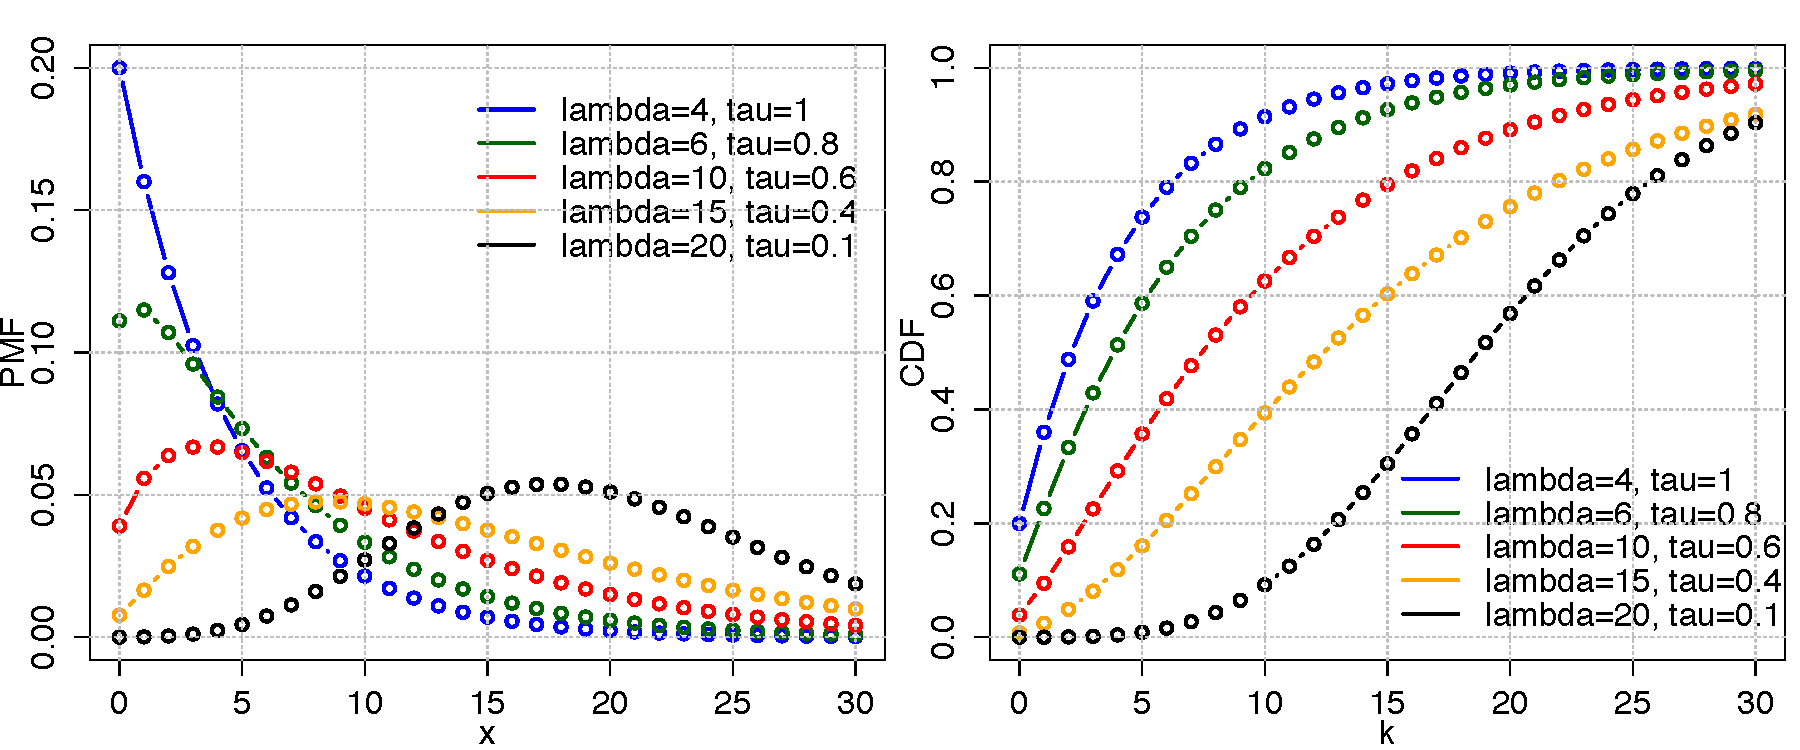
\includegraphics[width=140mm]{pics/NegativeBinomial2.pdf}
 \caption{NegativeBinomial2 distribution plotted using the provided R code.}
 \label{fig:NegativeBinomial2}
\end{figure}

\subsubsection*{Parameter: rate}

\noindent\begin{tabular}{p{2cm}cl}
\textbf{name} & & Poisson intensity \\
\textbf{type} & & scalar \\
\textbf{symbol} & & $\lambda$  \\
\textbf{definition} & & $\lambda \in R, \lambda > 0$
\end{tabular}
\subsubsection*{Parameter: overdispersion}

\noindent\begin{tabular}{p{2cm}cl}
\textbf{name} & & overdispersion \\
\textbf{type} & & scalar \\
\textbf{symbol} & & $\tau$  \\
\textbf{definition} & & $\tau \in R$
\end{tabular}
\subsubsection*{Functions}

\smallskip \noindent \hspace{.2cm} \textbf{PMF} 
\begin{equation*}\frac{\Gamma(k + \frac{1}{\tau})}{k!\; \Gamma(\frac{1}{\tau})} \Big(\frac{1}{1+\tau \lambda} \Big)^{\frac{1}{\tau}} 
\Big(\frac{\lambda}{\frac{1}{\tau} + \lambda} \Big)^{k}\end{equation*}
\smallskip \noindent \hspace{.2cm} \textbf{PMF in R}  
\begin{verbatim}
gamma(k+1/tau)/(factorial(k)*gamma(1/tau))*1/(1+tau*lambda)^(1/tau)*(lambda/(1/tau+lambda))^k
\end{verbatim}
\smallskip \noindent \hspace{.2cm} \textbf{CDF} 
\begin{equation*}\Sigma_{i=1}^x f(i), x \in \{0,1,2,...\}
\text { with f the PMF}\end{equation*}
\smallskip \noindent \hspace{.2cm} \textbf{CDF in R}  
\begin{verbatim}
cumsum(PMF)
\end{verbatim}
\smallskip
\subsubsection*{Characteristics}
\smallskip \noindent \hspace{.2cm} \textbf{Mean} 
\begin{equation*}\lambda\end{equation*}
\smallskip \noindent \hspace{.2cm} \textbf{Variance} 
\begin{equation*}\lambda (1 + \tau \lambda)\end{equation*}
\smallskip
%\section*{NegativeBinomial3} 
%
%  \bigskip 
%
%\begin{tabular}{p{2cm}cl}
%\textbf{name} & & Negative Binomial 3 (ID: 0000137)\\ 
% 
%\textbf{type} & & discrete \\ 
%
%\textbf{variate} & & $y$, scalar \\ 
%
%\textbf{support} & & $y \in \{0,1,2,3,\dots\}$
%\end{tabular}
%
%%\begin{figure}[ht!]
%%\centering
%%  \includegraphics[width=140mm]{pics/NegativeBinomial3.pdf}
%% \caption{NegativeBinomial3 distribution plotted using the provided R code.}
%% \label{fig:NegativeBinomial3}
%%\end{figure}
%
%\subsubsection*{Parameter: }
%
%\noindent\begin{tabular}{p{2cm}cl}
%\textbf{name} & & mean \\
%\textbf{type} & & scalar \\
%\textbf{symbol} & & $\mu$  \\
%\textbf{definition} & & $-$
%\end{tabular}
%\subsubsection*{Parameter: -}
%
%\noindent\begin{tabular}{p{2cm}cl}
%\textbf{name} & & size parameter \\
%\textbf{type} & & scalar \\
%\textbf{symbol} & & $\theta$  \\
%\textbf{definition} & & $-$
%\end{tabular}
%\subsubsection*{Functions}
%
%\smallskip \noindent \hspace{.2cm} \textbf{PMF} 
%\begin{equation*}\frac{\Gamma(\theta + y)}{\Gamma(a)\Gamma(y+1)} \Big(\frac{\theta}{\theta + \mu} \Big)^{\theta} 
%\Big(\frac{\mu}{\theta + \mu} \Big)^{y}\end{equation*}
%\smallskip \noindent \hspace{.2cm} \textbf{CDF} 
%\begin{equation*}-\end{equation*}
%\smallskip
%\subsubsection*{Characteristics}
%\smallskip \noindent \hspace{.2cm} \textbf{Mean} 
%\begin{equation*}\mu\end{equation*}
%\smallskip
\section*{Normal1} 

  \bigskip 

\begin{tabular}{p{2cm}cl}
\textbf{name} & & Normal 1 (ID: 0000148)\\ 
 
\textbf{type} & & continuous \\ 

\textbf{variate} & & $x$, scalar \\ 

\textbf{support} & & $x \in R$
\end{tabular}

\begin{figure}[ht!]
\centering
  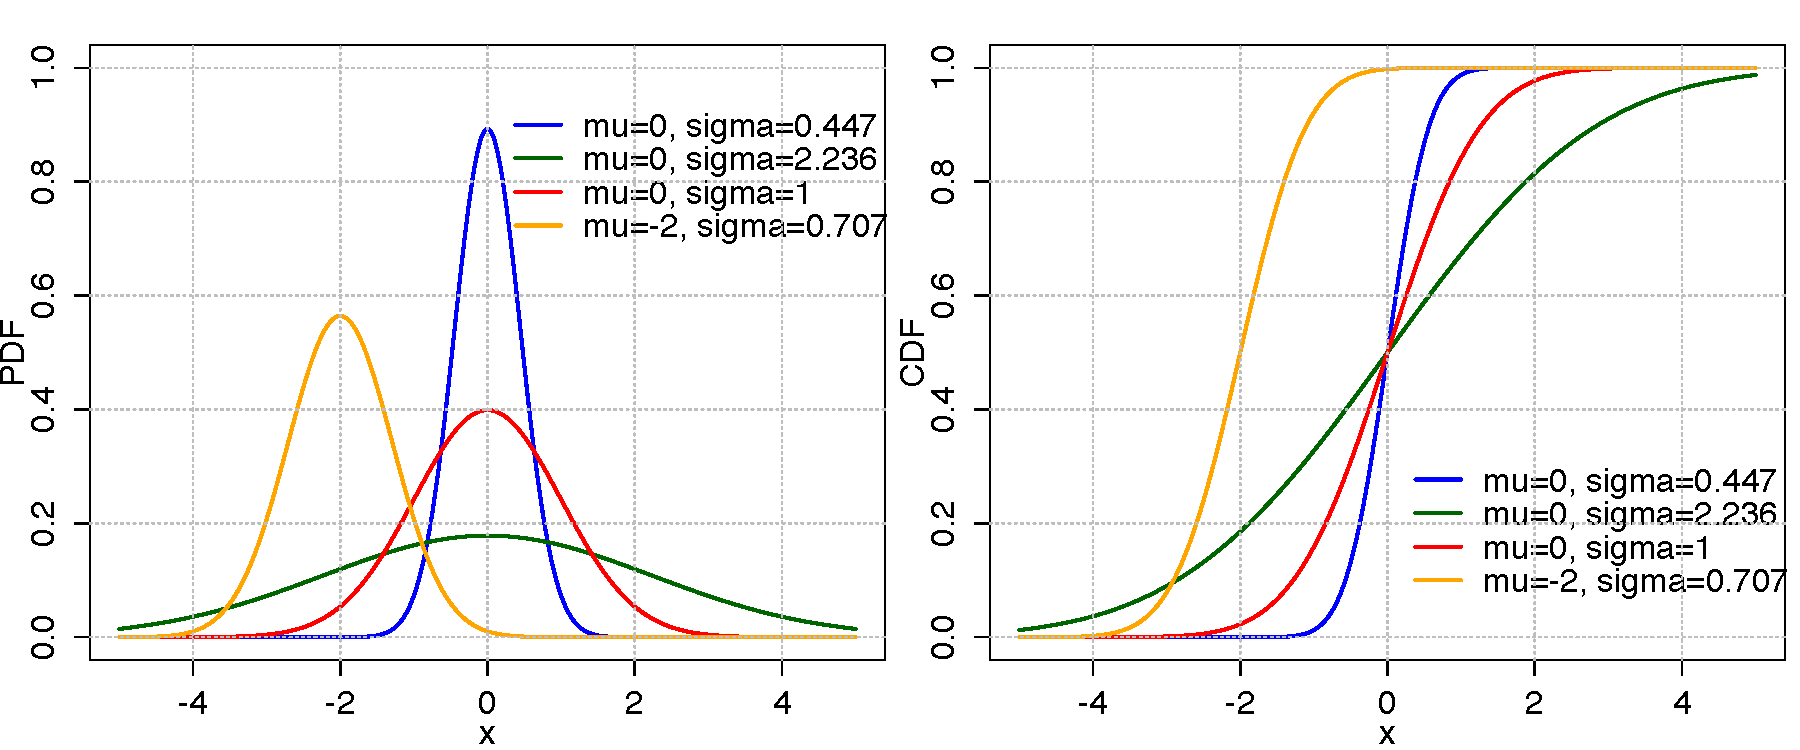
\includegraphics[width=140mm]{pics/Normal1.pdf}
 \caption{Normal1 distribution plotted using the provided R code.}
 \label{fig:Normal1}
\end{figure}

\subsubsection*{Parameter: mean}

\noindent\begin{tabular}{p{2cm}cl}
\textbf{name} & & mean \\
\textbf{type} & & scalar \\
\textbf{symbol} & & $\mu$  \\
\textbf{definition} & & $\mu \in R$
\end{tabular}
\subsubsection*{Parameter: stdev}

\noindent\begin{tabular}{p{2cm}cl}
\textbf{name} & & standard deviation \\
\textbf{type} & & scalar \\
\textbf{symbol} & & $\sigma$  \\
\textbf{definition} & & $\sigma> 0$
\end{tabular}
\subsubsection*{Functions}

\smallskip \noindent \hspace{.2cm} \textbf{PDF} 
\begin{equation*}\frac{1}{\sigma \sqrt{2 \pi}}e^{-\frac{(x-\mu)^2}{2\sigma^2}}\end{equation*}
\smallskip \noindent \hspace{.2cm} \textbf{PDF in R}  
\begin{verbatim}1/(sigma*sqrt(2*pi))*exp(-(x-mu)^2/(2*sigma^2))\end{verbatim}
\smallskip \noindent \hspace{.2cm} \textbf{CDF} 
\begin{equation*}\frac12\left[1 + \text{erf}\left( \frac{x-\mu}{\sigma\sqrt{2}}\right)\right]\end{equation*}
\smallskip \noindent \hspace{.2cm} \textbf{CDF in R} 
\begin{verbatim}1/2 * (1 + erf((x-mu)/(sigma*sqrt(2))))\end{verbatim}
\smallskip
\subsubsection*{Characteristics}
\smallskip \noindent \hspace{.2cm} \textbf{Mean} 
\begin{equation*}\mu\end{equation*}
\smallskip \noindent \hspace{.2cm} \textbf{Median} 
\begin{equation*}\mu\end{equation*}
\smallskip \noindent \hspace{.2cm} \textbf{Mode} 
\begin{equation*}\mu\end{equation*}
\smallskip \noindent \hspace{.2cm} \textbf{Variance} 
\begin{equation*}\sigma^2\end{equation*}
\smallskip
\section*{Normal2} 

  \bigskip 

\begin{tabular}{p{2cm}cl}
\textbf{name} & & Normal 2 (ID: 0000160)\\ 
 
\textbf{type} & & continuous \\ 

\textbf{variate} & & $x$, scalar \\ 

\textbf{support} & & $x \in R$
\end{tabular}

\begin{figure}[ht!]
\centering
  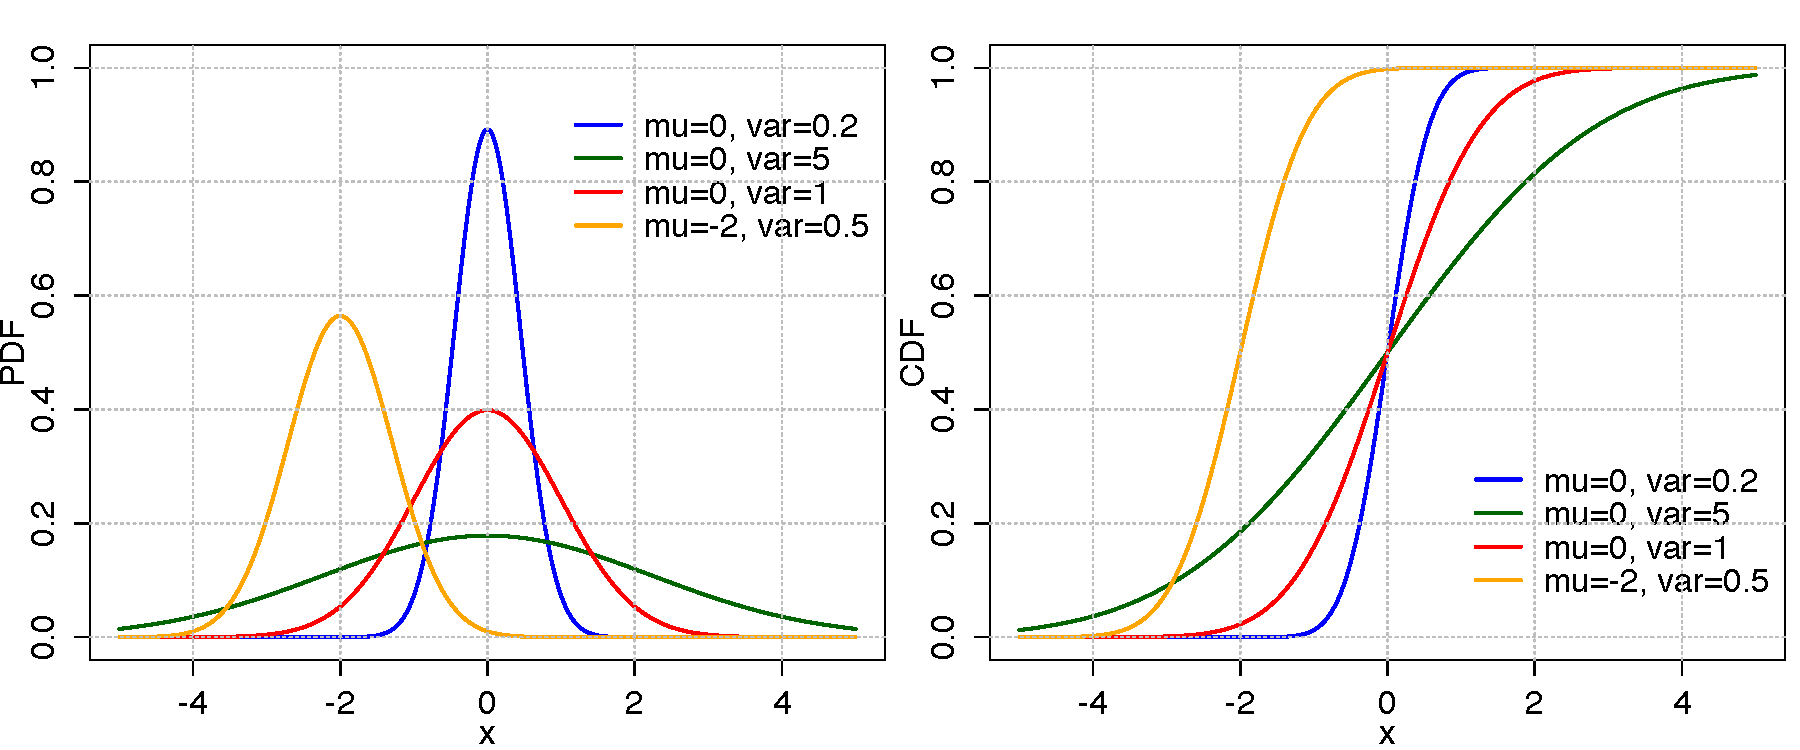
\includegraphics[width=140mm]{pics/Normal2.pdf}
 \caption{Normal2 distribution plotted using the provided R code.}
 \label{fig:Normal2}
\end{figure}

\subsubsection*{Parameter: mean}

\noindent\begin{tabular}{p{2cm}cl}
\textbf{name} & & mean \\
\textbf{type} & & scalar \\
\textbf{symbol} & & $\mu$  \\
\textbf{definition} & & $\mu \in R$
\end{tabular}
\subsubsection*{Parameter: var}

\noindent\begin{tabular}{p{2cm}cl}
\textbf{name} & & variance \\
\textbf{type} & & scalar \\
\textbf{symbol} & & $v$  \\
\textbf{definition} & & $v>0$
\end{tabular}
\subsubsection*{Functions}

\smallskip \noindent \hspace{.2cm} \textbf{PDF} 
\begin{equation*}\frac{1}{\sqrt{v} \sqrt{2 \pi}}e^{-\frac{(x-\mu)^2}{2*v}}\end{equation*}
\smallskip \noindent \hspace{.2cm} \textbf{PDF in R}  
\begin{verbatim}1/(sqrt(var)*sqrt(2*pi))*exp(-(x-mu)^2/(2*var))\end{verbatim}
\smallskip \noindent \hspace{.2cm} \textbf{CDF} 
\begin{equation*}\frac12\left[1 + \text{erf}\left( \frac{x-\mu}{\sqrt{v}\sqrt{2}}\right)\right]\end{equation*}
\smallskip \noindent \hspace{.2cm} \textbf{CDF in R} 
\begin{verbatim}1/2 * (1 + erf((x-mu)/(sqrt(var)*sqrt(2))))\end{verbatim}
\smallskip
\subsubsection*{Characteristics}
\smallskip \noindent \hspace{.2cm} \textbf{Mean} 
\begin{equation*}\mu\end{equation*}
\smallskip \noindent \hspace{.2cm} \textbf{Median} 
\begin{equation*}\mu\end{equation*}
\smallskip \noindent \hspace{.2cm} \textbf{Mode} 
\begin{equation*}\mu\end{equation*}
\smallskip \noindent \hspace{.2cm} \textbf{Variance} 
\begin{equation*}v\end{equation*}
\smallskip
\section*{Normal3} 

  \bigskip 

\begin{tabular}{p{2cm}cl}
\textbf{name} & & Normal 3 (ID: 0000170)\\ 
 
\textbf{type} & & continuous \\ 

\textbf{variate} & & $x$, scalar \\ 

\textbf{support} & & $x \in R$
\end{tabular}

\begin{figure}[ht!]
\centering
  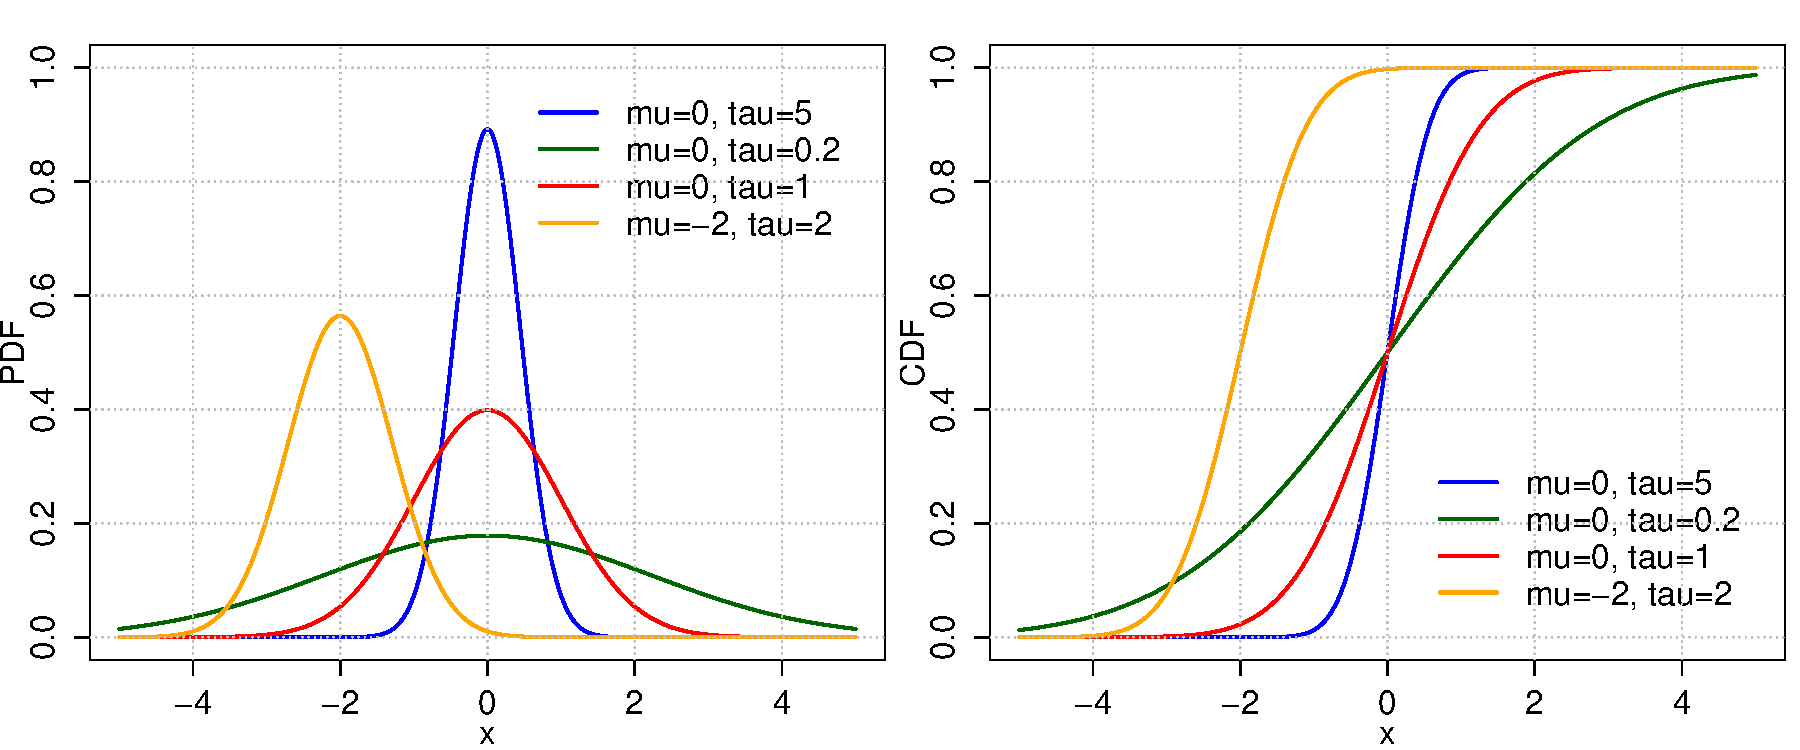
\includegraphics[width=140mm]{pics/Normal3.pdf}
 \caption{Normal3 distribution plotted using the provided R code.}
 \label{fig:Normal3}
\end{figure}

\subsubsection*{Parameter: mean}

\noindent\begin{tabular}{p{2cm}cl}
\textbf{name} & & mean \\
\textbf{type} & & scalar \\
\textbf{symbol} & & $\mu$  \\
\textbf{definition} & & $\mu \in R$
\end{tabular}
\subsubsection*{Parameter: precision}

\noindent\begin{tabular}{p{2cm}cl}
\textbf{name} & & precision \\
\textbf{type} & & scalar \\
\textbf{symbol} & & $\tau$  \\
\textbf{definition} & & $\tau>0$
\end{tabular}
\subsubsection*{Functions}

\smallskip \noindent \hspace{.2cm} \textbf{PDF} 
\begin{equation*}\sqrt{\frac{\tau}{2 \pi}} e^{-\frac{\tau}{2}(x-\mu)^2}\end{equation*}
\smallskip \noindent \hspace{.2cm} \textbf{PDF in R}  
\begin{verbatim}sqrt(tau/(2*pi))*exp(-tau/2*(x-mu)^2)\end{verbatim}
\smallskip \noindent \hspace{.2cm} \textbf{CDF} 
\begin{equation*}\frac12\left[1 + \text{erf}\left( \frac{x-\mu}{\sqrt{1/\tau}\sqrt{2}}\right)\right]\end{equation*}
\smallskip \noindent \hspace{.2cm} \textbf{CDF in R} 
\begin{verbatim}1/2*(1+erf((x-mu)/(sqrt(1/tau)*sqrt(2)))) \end{verbatim}
\smallskip
\subsubsection*{Characteristics}
\smallskip \noindent \hspace{.2cm} \textbf{Mean} 
\begin{equation*}\mu\end{equation*}
\smallskip \noindent \hspace{.2cm} \textbf{Median} 
\begin{equation*}\mu\end{equation*}
\smallskip \noindent \hspace{.2cm} \textbf{Mode} 
\begin{equation*}\mu\end{equation*}
\smallskip \noindent \hspace{.2cm} \textbf{Variance} 
\begin{equation*}1/\tau\end{equation*}
\smallskip
\section*{NormalInverseGamma1} 

  \bigskip 

\begin{tabular}{p{2cm}cl}
\textbf{name} & & Normal-inverse-gamma (ID: 0000180)\\ 
 
\textbf{type} & & continuous \\ 

\textbf{variate} & & $x$, scalar \\ 

\textbf{support} & & $x \in (-\infty,+\infty), \sigma^2 \in (0,+\infty)$
\end{tabular}

\begin{figure}[ht!]
\centering
  \includegraphics[width=70mm]{pics/NormalInverseGamma.pdf}
 \caption{NormalInverseGamma distribution plotted using the provided R code.}
 \label{fig:NormalInverseGamma}
\end{figure}

\subsubsection*{Parameter: mean}

\noindent\begin{tabular}{p{2cm}cl}
\textbf{name} & & location \\
\textbf{type} & & scalar \\
\textbf{symbol} & & $\mu$  \\
\textbf{definition} & & $\mu \in  R$
\end{tabular}
\subsubsection*{Parameter: lambda}

\noindent\begin{tabular}{p{2cm}cl}
\textbf{name} & & - \\
\textbf{type} & & scalar \\
\textbf{symbol} & & $\lambda$  \\
\textbf{definition} & & $\lambda > 0, \lambda \in  R$
\end{tabular}
\subsubsection*{Parameter: alpha}

\noindent\begin{tabular}{p{2cm}cl}
\textbf{name} & & shape \\
\textbf{type} & & scalar \\
\textbf{symbol} & & $\alpha$  \\
\textbf{definition} & & $\alpha > 0, \alpha \in  R$
\end{tabular}
\subsubsection*{Parameter: beta}

\noindent\begin{tabular}{p{2cm}cl}
\textbf{name} & & scale \\
\textbf{type} & & scalar \\
\textbf{symbol} & & $\beta$  \\
\textbf{definition} & & $\beta > 0, \beta \in  R$
\end{tabular}
\subsubsection*{Functions}

\smallskip \noindent \hspace{.2cm} \textbf{PDF} 
\begin{equation*}\frac {\sqrt{\lambda}} {\sigma\sqrt{2\pi} }  \frac{\beta^\alpha}{\Gamma(\alpha)} \, \left( \frac{1}{\sigma^2} \right)^{\alpha + 1}   e^{ -\frac { 2\beta + \lambda(x - \mu)^2} {2\sigma^2}  } \end{equation*}
\smallskip \noindent \hspace{.2cm} \textbf{PDF in R}  
\begin{verbatim}sqrt(lambda)/(sigma*sqrt(2*pi)) * beta^alpha/gamma(alpha) * (1/sigma^2)^(alpha + 1) * exp(- (2*beta+lambda*(x-mu)^2)/(2*sigma^2))\end{verbatim}
\smallskip \noindent \hspace{.2cm} \textbf{CDF} 
\begin{equation*}-\end{equation*}
\smallskip
\subsubsection*{Characteristics}
\smallskip
\section*{Pareto1} 

  \bigskip 

\begin{tabular}{p{2cm}cl}
\textbf{name} & & Pareto (ID: 0000192)\\ 
 
\textbf{type} & & continuous \\ 

\textbf{variate} & & $x$, scalar \\ 

\textbf{support} & & $x \in [x_m, +\infty)$
\end{tabular}

\begin{figure}[ht!]
\centering
  \includegraphics[width=140mm]{pics/Pareto.pdf}
 \caption{Pareto distribution plotted using the provided R code.}
 \label{fig:Pareto}
\end{figure}

\subsubsection*{Parameter: scale}

\noindent\begin{tabular}{p{2cm}cl}
\textbf{name} & & scale \\
\textbf{type} & & scalar \\
\textbf{symbol} & & $x_m$  \\
\textbf{definition} & & $x_m > 0, x_m \in R$
\end{tabular}
\subsubsection*{Parameter: shape}

\noindent\begin{tabular}{p{2cm}cl}
\textbf{name} & & shape \\
\textbf{type} & & scalar \\
\textbf{symbol} & & $\alpha$  \\
\textbf{definition} & & $\alpha > 0, \alpha \in R$
\end{tabular}
\subsubsection*{Functions}

\smallskip \noindent \hspace{.2cm} \textbf{PDF} 
\begin{equation*}\frac{\alpha\,x_m^\alpha}{x^{\alpha+1}}\text{ for }x\ge x_m\end{equation*}
\smallskip \noindent \hspace{.2cm} \textbf{PDF in R}  
\begin{verbatim}(alpha * x_m^alpha) / x^(alpha+1)\end{verbatim}
\smallskip \noindent \hspace{.2cm} \textbf{CDF} 
\begin{equation*}1-\left(\frac{x_m}{x}\right)^\alpha \text{ for } x \ge x_m\end{equation*}
\smallskip \noindent \hspace{.2cm} \textbf{CDF in R} 
\begin{verbatim}1-(x_m/x)^alpha\end{verbatim}
\smallskip
\subsubsection*{Characteristics}
\smallskip \noindent \hspace{.2cm} \textbf{Mean} 
\begin{equation*}\begin{cases}
\infty & \text{for }\alpha\le 1 \\
\frac{\alpha\,x_m}{\alpha-1} & \text{for }\alpha>1
\end{cases}\end{equation*}
\smallskip \noindent \hspace{.2cm} \textbf{Median} 
\begin{equation*}x_m \sqrt[\alpha]{2}\end{equation*}
\smallskip \noindent \hspace{.2cm} \textbf{Mode} 
\begin{equation*}x_m\end{equation*}
\smallskip \noindent \hspace{.2cm} \textbf{Variance} 
\begin{equation*}\begin{cases}
     \infty & \text{for }\alpha\in(1,2] \\
     \frac{x_m^2\alpha}{(\alpha-1)^2(\alpha-2)} & \text{for }\alpha>2
   \end{cases}\end{equation*}
\smallskip
\section*{Poisson1} 

  \bigskip 

\begin{tabular}{p{2cm}cl}
\textbf{name} & & Poisson (ID: 0000203)\\ 
 
\textbf{type} & & discrete \\ 

\textbf{variate} & & $k$, scalar \\ 

\textbf{support} & & $k \in \{0,1,2,3,\dots\}$
\end{tabular}

\begin{figure}[ht!]
\centering
  \includegraphics[width=140mm]{pics/Poisson.pdf}
 \caption{Poisson distribution plotted using the provided R code.}
 \label{fig:Poisson}
\end{figure}

\subsubsection*{Parameter: rate}

\noindent\begin{tabular}{p{2cm}cl}
\textbf{name} & & Poisson intensity \\
\textbf{type} & & scalar \\
\textbf{symbol} & & $\lambda$  \\
\textbf{definition} & & $\lambda \in R, \lambda > 0$
\end{tabular}
\subsubsection*{Functions}

\smallskip \noindent \hspace{.2cm} \textbf{PMF} 
\begin{equation*}\frac{\lambda^k}{k!}e^{-\lambda}\end{equation*}
\smallskip \noindent \hspace{.2cm} \textbf{PMF in R}  
\begin{verbatim}lambda^k/factorial(k) * exp(-lambda)\end{verbatim}
\smallskip \noindent \hspace{.2cm} \textbf{CDF} 
\begin{equation*}\frac{\gamma(\lfloor k+1 \rfloor,\lambda)}{\lfloor k \rfloor!}\end{equation*}
\smallskip \noindent \hspace{.2cm} \textbf{CDF in R} 
\begin{verbatim}Igamma(floor(k+1), lambda, lower=F) / factorial(floor(k))\end{verbatim}
\smallskip
\subsubsection*{Characteristics}
\smallskip \noindent \hspace{.2cm} \textbf{Mean} 
\begin{equation*}\lambda\end{equation*}
\smallskip \noindent \hspace{.2cm} \textbf{Median} 
\begin{equation*}\approx\lfloor\lambda+1/3-0.02/\lambda\rfloor\end{equation*}
\smallskip \noindent \hspace{.2cm} \textbf{Mode} 
\begin{equation*}\lceil\lambda\rceil - 1, \lfloor\lambda\rfloor\end{equation*}
\smallskip \noindent \hspace{.2cm} \textbf{Variance} 
\begin{equation*}\lambda\end{equation*}
\smallskip
\section*{Rayleigh1} 

  \bigskip 

\begin{tabular}{p{2cm}cl}
\textbf{name} & & Rayleigh (ID: 0000212)\\ 
 
\textbf{type} & & continuous \\ 

\textbf{variate} & & $x$, scalar \\ 

\textbf{support} & & $x \in [0,+\infty)$
\end{tabular}

\begin{figure}[ht!]
\centering
  \includegraphics[width=140mm]{pics/Rayleigh.pdf}
 \caption{Rayleigh distribution plotted using the provided R code.}
 \label{fig:Rayleigh}
\end{figure}

\subsubsection*{Parameter: scale}

\noindent\begin{tabular}{p{2cm}cl}
\textbf{name} & & scale \\
\textbf{type} & & scalar \\
\textbf{symbol} & & $\sigma$  \\
\textbf{definition} & & $\sigma > 0$
\end{tabular}
\subsubsection*{Functions}

\smallskip \noindent \hspace{.2cm} \textbf{PDF} 
\begin{equation*}\frac{x}{\sigma^2} e^{-x^2/2\sigma^2}\end{equation*}
\smallskip \noindent \hspace{.2cm} \textbf{PDF in R}  
\begin{verbatim}x/sigma^2 * exp(-x^2/(2*sigma^2))\end{verbatim}
\smallskip \noindent \hspace{.2cm} \textbf{CDF} 
\begin{equation*}1 - e^{-x^2/2\sigma^2}\end{equation*}
\smallskip \noindent \hspace{.2cm} \textbf{CDF in R} 
\begin{verbatim}1 - exp(-x^2/(2*sigma^2))\end{verbatim}
\smallskip
\subsubsection*{Characteristics}
\smallskip \noindent \hspace{.2cm} \textbf{Mean} 
\begin{equation*}\sigma \sqrt{\frac{\pi}{2}}\end{equation*}
\smallskip \noindent \hspace{.2cm} \textbf{Median} 
\begin{equation*}\sigma \sqrt{\log(4)}\end{equation*}
\smallskip \noindent \hspace{.2cm} \textbf{Mode} 
\begin{equation*}\sigma\end{equation*}
\smallskip \noindent \hspace{.2cm} \textbf{Variance} 
\begin{equation*}\frac{4 - \pi}{2} \sigma^2\end{equation*}
\smallskip
\section*{StandardNormal1}

  \bigskip 

\begin{tabular}{p{2cm}cl}
\textbf{name} & & Standard Normal (ID: 0000221)\\ 
 
\textbf{type} & & continuous \\ 

\textbf{variate} & & $x$, scalar \\ 

\textbf{support} & & $x \in R$
\end{tabular}

\begin{figure}[ht!]
\centering
  \includegraphics[width=140mm]{pics/StandardNormal.pdf}
 \caption{StandardNormal distribution plotted using the provided R code.}
 \label{fig:StandardNormal}
\end{figure}

\subsubsection*{Parameter: mean}

\noindent\begin{tabular}{p{2cm}cl}
\textbf{name} & & mean \\
\textbf{type} & & scalar \\
\textbf{symbol} & & $\mu$  \\
\textbf{definition} & & $\mu=0$
\end{tabular}
\subsubsection*{Parameter: stdev}

\noindent\begin{tabular}{p{2cm}cl}
\textbf{name} & & standard deviation \\
\textbf{type} & & scalar \\
\textbf{symbol} & & $\sigma$  \\
\textbf{definition} & & $\sigma=1$
\end{tabular}
\subsubsection*{Functions}

\smallskip \noindent \hspace{.2cm} \textbf{PDF} 
\begin{equation*}\frac{e^{-\frac{1}{2} x^2}}{\sqrt{2\pi}}\end{equation*}
\smallskip \noindent \hspace{.2cm} \textbf{PDF in R}  
\begin{verbatim}1/(sqrt(2*pi))*exp(-x^2/2)\end{verbatim}
\smallskip \noindent \hspace{.2cm} \textbf{CDF} 
\begin{equation*}\frac12\left[1 + \text{erf}\left( \frac{x}{\sqrt{2}}\right)\right]\end{equation*}
\smallskip \noindent \hspace{.2cm} \textbf{CDF in R} 
\begin{verbatim}1/2 * (1 + erf(x/(sqrt(2))))\end{verbatim}
\smallskip
\subsubsection*{Characteristics}
\smallskip \noindent \hspace{.2cm} \textbf{Mean} 
\begin{equation*}0\end{equation*}
\smallskip \noindent \hspace{.2cm} \textbf{Median} 
\begin{equation*}0\end{equation*}
\smallskip \noindent \hspace{.2cm} \textbf{Mode} 
\begin{equation*}0\end{equation*}
\smallskip \noindent \hspace{.2cm} \textbf{Variance} 
\begin{equation*}1\end{equation*}
\smallskip
\section*{StandardUniform1} 

  \bigskip 

\begin{tabular}{p{2cm}cl}
\textbf{name} & & Standard Uniform (ID: 0000240)\\ 
 
\textbf{type} & & continuous \\ 

\textbf{variate} & & $x$, scalar \\ 

\textbf{support} & & $x \in [0,1]$
\end{tabular}

\begin{figure}[ht!]
\centering
  \includegraphics[width=140mm]{pics/StandardUniform.pdf}
 \caption{StandardUniform distribution plotted using the provided R code.}
 \label{fig:StandardUniform}
\end{figure}

\subsubsection*{Parameter: minimum}

\noindent\begin{tabular}{p{2cm}cl}
\textbf{name} & & minimum \\
\textbf{type} & & scalar \\
\textbf{symbol} & & $a$  \\
\textbf{definition} & & $a=0$
\end{tabular}
\subsubsection*{Parameter: maximum}

\noindent\begin{tabular}{p{2cm}cl}
\textbf{name} & & maximum \\
\textbf{type} & & scalar \\
\textbf{symbol} & & $b$  \\
\textbf{definition} & & $b=1$
\end{tabular}
\subsubsection*{Functions}

\smallskip \noindent \hspace{.2cm} \textbf{PDF} 
\begin{equation*}1\end{equation*}
\smallskip \noindent \hspace{.2cm} \textbf{PDF in R}  
\begin{verbatim}1\end{verbatim}
\smallskip \noindent \hspace{.2cm} \textbf{CDF} 
\begin{equation*}x\end{equation*}
\smallskip \noindent \hspace{.2cm} \textbf{CDF in R} 
\begin{verbatim}x\end{verbatim}
\smallskip
\subsubsection*{Characteristics}
\smallskip \noindent \hspace{.2cm} \textbf{Mean} 
\begin{equation*}0.5\end{equation*}
\smallskip \noindent \hspace{.2cm} \textbf{Median} 
\begin{equation*}0.5\end{equation*}
\smallskip \noindent \hspace{.2cm} \textbf{Mode} 
\begin{equation*}\text{any value in }[0,1]\end{equation*}
\smallskip
\section*{StudentT1} 

  \bigskip 

\begin{tabular}{p{2cm}cl}
\textbf{name} & & Student's t-distribution (ID: 0000231)\\ 
 
\textbf{type} & & continuous \\ 

\textbf{variate} & & $x$, scalar \\ 

\textbf{support} & & $x \in (-\infty,+\infty)$
\end{tabular}

\begin{figure}[ht!]
\centering
  \includegraphics[width=140mm]{pics/StudentT.pdf}
 \caption{StudentT distribution plotted using the provided R code.}
 \label{fig:StudentT}
\end{figure}

\subsubsection*{Parameter: degreesOfFreedom}

\noindent\begin{tabular}{p{2cm}cl}
\textbf{name} & & degrees of freedom \\
\textbf{type} & & scalar \\
\textbf{symbol} & & $\nu$  \\
\textbf{definition} & & $\nu > 0, \nu \in  R$
\end{tabular}
\subsubsection*{Functions}

\smallskip \noindent \hspace{.2cm} \textbf{PDF} 
\begin{equation*}\frac{\Gamma \left(\frac{\nu+1}{2} \right)} {\sqrt{\nu\pi}\,\Gamma \left(\frac{\nu}{2} \right)} \left(1+\frac{x^2}{\nu} \right)^{-\frac{\nu+1}{2}}\end{equation*}
\smallskip \noindent \hspace{.2cm} \textbf{PDF in R}  
\begin{verbatim}gamma((nu+1)/2)/(sqrt(nu*pi)*gamma(nu/2))*(1+x^2/nu)^(-(nu+1)/2)\end{verbatim}
\smallskip \noindent \hspace{.2cm} \textbf{CDF} 
\begin{equation*}\begin{matrix}
     \frac{1}{2} + x \Gamma \left( \frac{\nu+1}{2} \right)  \times
     \frac{\,_2F_1 \left ( \frac{1}{2},\frac{\nu+1}{2};\frac{3}{2};
           -\frac{x^2}{\nu} \right)}
     {\sqrt{\pi\nu}\,\Gamma \left(\frac{\nu}{2}\right)}
     \end{matrix}\end{equation*}
\smallskip \noindent \hspace{.2cm} \textbf{CDF in R} 
\begin{verbatim}1/2+x*gamma((nu+1)/2)*hypergeo(1/2,(nu+1)/2,3/2,-x^2/nu)/( sqrt(pi*nu) *gamma(nu/2))\end{verbatim}
\smallskip
\subsubsection*{Characteristics}
\smallskip \noindent \hspace{.2cm} \textbf{Mean} 
\begin{equation*}\begin{cases}
0 & \text{for }\nu > 0 \\ undefined & \text{else} 
\end{cases}\end{equation*}
\smallskip \noindent \hspace{.2cm} \textbf{Median} 
\begin{equation*}0\end{equation*}
\smallskip \noindent \hspace{.2cm} \textbf{Mode} 
\begin{equation*}0\end{equation*}
\smallskip \noindent \hspace{.2cm} \textbf{Variance} 
\begin{equation*}\begin{cases}
\frac{\nu}{\nu - 2} & \text{for }\nu > 2 \\
\infty & \text{for } 1< \nu \leq 2 \\
undefined & \text{else} 
\end{cases}\end{equation*}
\smallskip
\section*{Triangular1} 

  \bigskip 

\begin{tabular}{p{2cm}cl}
\textbf{name} & & Triangular (ID: 0000250)\\ 
 
\textbf{type} & & continuous \\ 

\textbf{variate} & & $x$, scalar \\ 

\textbf{support} & & $a \leq x \leq b$
\end{tabular}

\begin{figure}[ht!]
\centering
  \includegraphics[width=140mm]{pics/Triangular.pdf}
 \caption{Triangular distribution plotted using the provided R code.}
 \label{fig:Triangular}
\end{figure}

\subsubsection*{Parameter: lowerLimit}

\noindent\begin{tabular}{p{2cm}cl}
\textbf{name} & & lower limit \\
\textbf{type} & & scalar \\
\textbf{symbol} & & $a$  \\
\textbf{definition} & & $a \in R$
\end{tabular}
\subsubsection*{Parameter: upperLimit}

\noindent\begin{tabular}{p{2cm}cl}
\textbf{name} & & upper limit \\
\textbf{type} & & scalar \\
\textbf{symbol} & & $b$  \\
\textbf{definition} & & $b \in R, a < b$
\end{tabular}
\subsubsection*{Parameter: shape}

\noindent\begin{tabular}{p{2cm}cl}
\textbf{name} & & shape (mode) \\
\textbf{type} & & scalar \\
\textbf{symbol} & & $c$  \\
\textbf{definition} & & $c \in R$
\end{tabular}
\subsubsection*{Functions}

\smallskip \noindent \hspace{.2cm} \textbf{PDF} 
\begin{equation*}\begin{cases}
2(x-a) / [(b-a)(c-a)] & \text{ for } a \leq x \leq c \\
2(b-x) / [(b-a)(b-c)] & \text{ for } c \leq x \leq b
\end{cases}\end{equation*}
\smallskip \noindent \hspace{.2cm} \textbf{PDF in R}  
\begin{verbatim}2*(x-a) / ((b-a)*(c-a)) for a <= x <= c \\
2*(b-x) / ((b-a)*(b-c)) for c <= x <= b \end{verbatim}
\smallskip \noindent \hspace{.2cm} \textbf{CDF} 
\begin{equation*}\begin{cases}
(x-a)^2 / [(b-a)(c-a)] & \text{ for } a \leq x \leq c \\
1 - (b-x)^2 / [(b-a)(b-c)] & \text{ for } c \leq x \leq b
\end{cases}\end{equation*}
\smallskip \noindent \hspace{.2cm} \textbf{CDF in R} 
\begin{verbatim}(x-a)^2 / ((b-a)*(c-a)) for a <= x <= c \\
1 - (b-x)^2 / ((b-a)*(b-c)) for c <= x <= b \end{verbatim}
\smallskip
\subsubsection*{Characteristics}
\smallskip \noindent \hspace{.2cm} \textbf{Mean} 
\begin{equation*}(a+b+c)/3\end{equation*}
\smallskip \noindent \hspace{.2cm} \textbf{Mode} 
\begin{equation*}c\end{equation*}
\smallskip \noindent \hspace{.2cm} \textbf{Variance} 
\begin{equation*}(a^2 + b^2 + c^2 - ab - ac - bc)/18\end{equation*}
\smallskip
\section*{TruncatedNormal1} 

  \bigskip 

\begin{tabular}{p{2cm}cl}
\textbf{name} & & Truncated Normal (ID: 0000261)\\ 
 
\textbf{type} & & continuous \\ 

\textbf{variate} & & $x$, scalar \\ 

\textbf{support} & & $x \in [a,b]$
\end{tabular}

\begin{figure}[ht!]
\centering
  \includegraphics[width=140mm]{pics/TruncatedNormal.pdf}
 \caption{TruncatedNormal distribution plotted using the provided R code.}
 \label{fig:TruncatedNormal}
\end{figure}

\subsubsection*{Parameter: mean}

\noindent\begin{tabular}{p{2cm}cl}
\textbf{name} & & mean \\
\textbf{type} & & scalar \\
\textbf{symbol} & & $\mu$  \\
\textbf{definition} & & $\mu \in R$
\end{tabular}
\subsubsection*{Parameter: stdev}

\noindent\begin{tabular}{p{2cm}cl}
\textbf{name} & & standard deviation \\
\textbf{type} & & scalar \\
\textbf{symbol} & & $\sigma$  \\
\textbf{definition} & & $\sigma > 0$
\end{tabular}
\subsubsection*{Parameter: lowerBound}

\noindent\begin{tabular}{p{2cm}cl}
\textbf{name} & & lower bound \\
\textbf{type} & & scalar \\
\textbf{symbol} & & $a$  \\
\textbf{definition} & & $a \in R$
\end{tabular}
\subsubsection*{Parameter: upperBound}

\noindent\begin{tabular}{p{2cm}cl}
\textbf{name} & & upper bound \\
\textbf{type} & & scalar \\
\textbf{symbol} & & $b$  \\
\textbf{definition} & & $b \in R, b > a$
\end{tabular}
\subsubsection*{Functions}

\smallskip \noindent \hspace{.2cm} \textbf{PDF} 
\begin{equation*}\frac{\frac{1}{\sigma} \phi(\frac{x-\mu}{\sigma})}{\Phi(\frac{b-\mu}{\sigma})-\Phi(\frac{a-\mu}{\sigma})}\end{equation*}
\smallskip \noindent \hspace{.2cm} \textbf{PDF in R}  
\begin{verbatim}( 1/sigma * phi((x-mu)/sigma) ) / ( Phi((b-mu)/sigma)-Phi((a-mu)/sigma) )\end{verbatim}
\smallskip \noindent \hspace{.2cm} \textbf{CDF} 
\begin{equation*}\frac{\Phi(\frac{x-\mu}{\sigma})-\Phi(\frac{a-\mu}{\sigma})}{\Phi(\frac{b-\mu}{\sigma})-\Phi(\frac{a-\mu}{\sigma})}\end{equation*}
\smallskip \noindent \hspace{.2cm} \textbf{CDF in R} 
\begin{verbatim}( Phi((x-mu)/sigma)-Phi((a-mu)/sigma) ) / ( Phi((b-mu)/sigma)-Phi((a-mu)/sigma) )\end{verbatim}
\smallskip
\subsubsection*{Characteristics}
\smallskip \noindent \hspace{.2cm} \textbf{Mean} 
\begin{equation*}
\mu + \frac{ \phi(\frac{a-\mu}{\sigma}) - \phi(\frac{b-\mu}{\sigma}) }{ \Phi(\frac{b-\mu}{\sigma}) - \Phi(\frac{a-\mu}{\sigma}) } \sigma
\end{equation*}
\smallskip \noindent \hspace{.2cm} \textbf{Variance} 
\begin{equation*}\sigma^2 \Big[ 1 
+ \frac{ \frac{a-\mu}{\sigma}\phi(\frac{a-\mu}{\sigma}) - \frac{b-\mu}{\sigma}\phi(\frac{b-\mu}{\sigma}) }{ \Phi(\frac{b-\mu}{\sigma}) - \Phi(\frac{a-\mu}{\sigma}) } 
- \Big( \frac{ \phi(\frac{a-\mu}{\sigma}) - \phi(\frac{b-\mu}{\sigma}) }{ \Phi(\frac{b-\mu}{\sigma}) - \Phi(\frac{a-\mu}{\sigma}) } \Big)^2 \Big]\end{equation*}
\smallskip
\section*{Uniform1} 

  \bigskip 

\begin{tabular}{p{2cm}cl}
\textbf{name} & & Uniform (ID: 0000273)\\ 
 
\textbf{type} & & continuous \\ 

\textbf{variate} & & $x$, scalar \\ 

\textbf{support} & & $x \in [a,b]$
\end{tabular}

\begin{figure}[ht!]
\centering
  \includegraphics[width=140mm]{pics/Uniform.pdf}
 \caption{Uniform distribution plotted using the provided R code.}
 \label{fig:Uniform}
\end{figure}

\subsubsection*{Parameter: minimum}

\noindent\begin{tabular}{p{2cm}cl}
\textbf{name} & & minimum \\
\textbf{type} & & scalar \\
\textbf{symbol} & & $a$  \\
\textbf{definition} & & $a \in  R$
\end{tabular}
\subsubsection*{Parameter: maximum}

\noindent\begin{tabular}{p{2cm}cl}
\textbf{name} & & maximum \\
\textbf{type} & & scalar \\
\textbf{symbol} & & $b$  \\
\textbf{definition} & & $b \in R, a < b$
\end{tabular}
\subsubsection*{Functions}

\smallskip \noindent \hspace{.2cm} \textbf{PDF} 
\begin{equation*}\begin{cases}
                  \frac{1}{b - a} & \text{for } x \in [a,b]  \\
                  0               & \text{otherwise}
                \end{cases}\end{equation*}
\smallskip \noindent \hspace{.2cm} \textbf{PDF in R}  
\begin{verbatim}1/(b-a)\end{verbatim}
\smallskip \noindent \hspace{.2cm} \textbf{CDF} 
\begin{equation*}\begin{cases}
                  0               & \text{for } x < a \\
                  \frac{x-a}{b-a} & \text{for } x \in [a,b) \\
                  1               & \text{for } x \ge b
                \end{cases}\end{equation*}
\smallskip \noindent \hspace{.2cm} \textbf{CDF in R} 
\begin{verbatim}(x-a)/(b-a)\end{verbatim}
\smallskip
\subsubsection*{Characteristics}
\smallskip \noindent \hspace{.2cm} \textbf{Mean} 
\begin{equation*}\tfrac{1}{2}(a+b)\end{equation*}
\smallskip \noindent \hspace{.2cm} \textbf{Median} 
\begin{equation*}\tfrac{1}{2}(a+b)\end{equation*}
\smallskip \noindent \hspace{.2cm} \textbf{Mode} 
\begin{equation*}\text{any value in }[a,b]\end{equation*}
\smallskip \noindent \hspace{.2cm} \textbf{Variance} 
\begin{equation*}\tfrac{1}{12} (b-a)^2\end{equation*}
\smallskip
\section*{UniformDiscrete1} 

  \bigskip 

\begin{tabular}{p{2cm}cl}
\textbf{name} & & Uniform Discrete 1 (ID: 0000283)\\ 
 
\textbf{type} & & discrete \\ 

\textbf{variate} & & $k$, scalar \\ 

\textbf{support} & & $k \in \{a,a+1,...,b-1,b\}$
\end{tabular}

\begin{figure}[ht!]
\centering
  \includegraphics[width=140mm]{pics/UniformDiscrete1.pdf}
 \caption{UniformDiscrete1 distribution plotted using the provided R code.}
 \label{fig:UniformDiscrete1}
\end{figure}

\subsubsection*{Parameter: minimum}

\noindent\begin{tabular}{p{2cm}cl}
\textbf{name} & & minimum \\
\textbf{type} & & scalar \\
\textbf{symbol} & & $a$  \\
\textbf{definition} & & $a \in \{\dots,-2,-1,0,1,2,3,\dots\}$
\end{tabular}
\subsubsection*{Parameter: maximum}

\noindent\begin{tabular}{p{2cm}cl}
\textbf{name} & & maximum \\
\textbf{type} & & scalar \\
\textbf{symbol} & & $b$  \\
\textbf{definition} & & $b \in \{\dots,-2,-1,0,1,2,3,\dots\}, b \ge a$
\end{tabular}
%\subsubsection*{Parameter: numberOfValues}
%
%\noindent\begin{tabular}{p{2cm}cl}
%\textbf{name} & & number of values \\
%\textbf{type} & & scalar \\
%\textbf{symbol} & & $n$  \\
%\textbf{definition} & & $n=b-a+1$
%\end{tabular}
\subsubsection*{Functions}

\smallskip \noindent \hspace{.2cm} \textbf{PMF} 
\begin{equation*}1/(b-a+1)\end{equation*}
\smallskip \noindent \hspace{.2cm} \textbf{PMF in R}  
\begin{verbatim}1/(b-a+1)\end{verbatim}
\smallskip \noindent \hspace{.2cm} \textbf{CDF} 
\begin{equation*}\frac{\lfloor k \rfloor -a+1}{b-a+1}\end{equation*}
\smallskip \noindent \hspace{.2cm} \textbf{CDF in R} 
\begin{verbatim}(floor(k)-a+1)/b-a+1\end{verbatim}
\smallskip
\subsubsection*{Characteristics}
\smallskip \noindent \hspace{.2cm} \textbf{Mean} 
\begin{equation*}\tfrac{1}{2}(a+b)\end{equation*}
\smallskip \noindent \hspace{.2cm} \textbf{Median} 
\begin{equation*}\tfrac{1}{2}(a+b)\end{equation*}
\smallskip \noindent \hspace{.2cm} \textbf{Mode} 
\begin{equation*}NA\end{equation*}
\smallskip \noindent \hspace{.2cm} \textbf{Variance} 
\begin{equation*}\frac{(b-a+1)^2 -1}{12}\end{equation*}
\smallskip
\section*{UniformDiscrete2} 

  \bigskip 

\begin{tabular}{p{2cm}cl}
\textbf{name} & & Uniform Discrete 2 (ID: 0000294)\\ 
 
\textbf{type} & & discrete \\ 

\textbf{variate} & & $k$, scalar \\ 

\textbf{support} & & $k \in \{0,1,2,\dots,n\}$
\end{tabular}

\begin{figure}[ht!]
\centering
  \includegraphics[width=140mm]{pics/UniformDiscrete2.pdf}
 \caption{UniformDiscrete2 distribution plotted using the provided R code.}
 \label{fig:UniformDiscrete2}
\end{figure}

\subsubsection*{Parameter: minimum}

\noindent\begin{tabular}{p{2cm}cl}
\textbf{name} & & minimum \\
\textbf{type} & & scalar \\
\textbf{symbol} & & $a$  \\
\textbf{definition} & & $a=0$
\end{tabular}
\subsubsection*{Parameter: numberOfValues}

\noindent\begin{tabular}{p{2cm}cl}
\textbf{name} & & number of values \\
\textbf{type} & & scalar \\
\textbf{symbol} & & $n$  \\
\textbf{definition} & & $n \in N$
\end{tabular}
\subsubsection*{Functions}

\smallskip \noindent \hspace{.2cm} \textbf{PMF} 
\begin{equation*}1/(n+1)\end{equation*}
\smallskip \noindent \hspace{.2cm} \textbf{PMF in R}  
\begin{verbatim}1/(n+1)\end{verbatim}
\smallskip \noindent \hspace{.2cm} \textbf{CDF} 
\begin{equation*}\frac{k+1}{n+1}\end{equation*}
\smallskip \noindent \hspace{.2cm} \textbf{CDF in R} 
\begin{verbatim}(k+1)/(n+1)\end{verbatim}
\smallskip
\subsubsection*{Characteristics}
\smallskip \noindent \hspace{.2cm} \textbf{Mean} 
\begin{equation*}\frac{n}{2}\end{equation*}
\smallskip \noindent \hspace{.2cm} \textbf{Variance} 
\begin{equation*}\frac{n(n+2)}{12}\end{equation*}
\smallskip
\section*{Weibull1} 

  \bigskip 

\begin{tabular}{p{2cm}cl}
\textbf{name} & & Weibull 1 (ID: 0000304)\\ 
 
\textbf{type} & & continuous \\ 

\textbf{variate} & & $x$, scalar \\ 

\textbf{support} & & $x \in [0,+\infty)$
\end{tabular}

\begin{figure}[ht!]
\centering
  \includegraphics[width=140mm]{pics/Weibull1.pdf}
 \caption{Weibull1 distribution plotted using the provided R code.}
 \label{fig:Weibull1}
\end{figure}

\subsubsection*{Parameter: scale}

\noindent\begin{tabular}{p{2cm}cl}
\textbf{name} & & scale \\
\textbf{type} & & scalar \\
\textbf{symbol} & & $\lambda$  \\
\textbf{definition} & & $\lambda\in (0, +\infty)$
\end{tabular}
\subsubsection*{Parameter: shape}

\noindent\begin{tabular}{p{2cm}cl}
\textbf{name} & & shape \\
\textbf{type} & & scalar \\
\textbf{symbol} & & $k$  \\
\textbf{definition} & & $k\in (0, +\infty)$
\end{tabular}
\subsubsection*{Functions}

\smallskip \noindent \hspace{.2cm} \textbf{PDF} 
\begin{equation*}\begin{cases}
\frac{k}{\lambda}\left(\frac{x}{\lambda}\right)^{k-1}e^{-(x/\lambda)^{k}} & x\geq0\\
0 & x<0\end{cases}\end{equation*}
\smallskip \noindent \hspace{.2cm} \textbf{PDF in R}  
\begin{verbatim}k/lambda * (x/lambda)^(k-1) * exp(-(x/lambda)^k)\end{verbatim}
\smallskip \noindent \hspace{.2cm} \textbf{CDF} 
\begin{equation*}\begin{cases}1- e^{-(x/\lambda)^k} & x\geq0\\ 0 & x<0\end{cases}\end{equation*}
\smallskip \noindent \hspace{.2cm} \textbf{CDF in R} 
\begin{verbatim}1- exp(-(x/lambda)^k)\end{verbatim}
\smallskip
\subsubsection*{Characteristics}
\smallskip \noindent \hspace{.2cm} \textbf{Mean} 
\begin{equation*}\lambda \, \Gamma(1+1/k)\end{equation*}
\smallskip \noindent \hspace{.2cm} \textbf{Median} 
\begin{equation*}\lambda(\log(2))^{1/k}\end{equation*}
\smallskip \noindent \hspace{.2cm} \textbf{Mode} 
\begin{equation*}\begin{cases}
\lambda \left(\frac{k-1}{k} \right)^{\frac{1}{k}}\, &k>1\\
0 &k=1\end{cases}\end{equation*}
\smallskip \noindent \hspace{.2cm} \textbf{Variance} 
\begin{equation*}\lambda^2\left[\Gamma\left(1+\frac{2}{k}\right) - \left(\Gamma\left(1+\frac{1}{k}\right)\right)^2\right]\end{equation*}
\smallskip
\section*{Weibull2} 

  \bigskip 

\begin{tabular}{p{2cm}cl}
\textbf{name} & & Weibull 2 (ID: 0000314)\\ 
 
\textbf{type} & & continuous \\ 

\textbf{variate} & & $x$, scalar \\ 

\textbf{support} & & $x > 0$
\end{tabular}

\begin{figure}[ht!]
\centering
  \includegraphics[width=140mm]{pics/Weibull2.pdf}
 \caption{Weibull2 distribution plotted using the provided R code.}
 \label{fig:Weibull2}
\end{figure}

\subsubsection*{Parameter: lambda}

\noindent\begin{tabular}{p{2cm}cl}
\textbf{name} & & lambda \\
\textbf{type} & & scalar \\
\textbf{symbol} & & $\lambda$  \\
\textbf{definition} & & $-$
\end{tabular}
\subsubsection*{Parameter: shape}

\noindent\begin{tabular}{p{2cm}cl}
\textbf{name} & & shape \\
\textbf{type} & & scalar \\
\textbf{symbol} & & $v$  \\
\textbf{definition} & & $-$
\end{tabular}
\subsubsection*{Functions}

\smallskip \noindent \hspace{.2cm} \textbf{PDF} 
\begin{equation*}v\lambda \,x^{v-1} e^{-\lambda x^{v}}\end{equation*}
\smallskip \noindent \hspace{.2cm} \textbf{PDF in R}  
\begin{verbatim}v*lambda * x^(v-1) * exp(-lambda * x^v)\end{verbatim}
\smallskip \noindent \hspace{.2cm} \textbf{CDF} 
\begin{equation*}1- e^{-x^v \lambda}\end{equation*}
\smallskip \noindent \hspace{.2cm} \textbf{CDF in R} 
\begin{verbatim}1- exp(-x^v * lambda)\end{verbatim}
\smallskip
\subsubsection*{Characteristics}
%\smallskip \noindent \hspace{.2cm} \textbf{Mean} 
%\begin{equation*}-\end{equation*}
\smallskip
\section*{Wishart1} 

  \bigskip 

\begin{tabular}{p{2cm}cl}
\textbf{name} & & Wishart 1 (ID: 0000324)\\ 
 
\textbf{type} & & continuous \\ 

\textbf{variate} & & $X$, matrix \\ 

\textbf{support} & & $X(p \times p) - \text{positive definite matrix}$
\end{tabular}

%\begin{figure}[ht!]
%\centering
%  \includegraphics[width=140mm]{pics/Wishart1.pdf}
% \caption{Wishart1 distribution plotted using the provided R code.}
% \label{fig:Wishart1}
%\end{figure}

\subsubsection*{Parameter: scaleMatrix}

\noindent\begin{tabular}{p{2cm}cl}
\textbf{name} & & scale matrix \\
\textbf{type} & & matrix \\
\textbf{symbol} & & $V$  \\
\textbf{definition} & & $V > 0, p\times p - \text{positive definite matrix}$
\end{tabular}
\subsubsection*{Parameter: degreesOfFreedom}

\noindent\begin{tabular}{p{2cm}cl}
\textbf{name} & & degrees of freedom \\
\textbf{type} & & scalar \\
\textbf{symbol} & & $n$  \\
\textbf{definition} & & $n > p-1$
\end{tabular}
\subsubsection*{Functions}

\smallskip \noindent \hspace{.2cm} \textbf{PDF} 
\begin{equation*}\frac{|X|^{\frac{n-p-1}{2}} e^{-\frac{\text{tr}(V^{-1}X)}{2}}}{2^\frac{np}{2}|V|^\frac{n}{2}\Gamma_p(\frac{n}{2})}\end{equation*}
\smallskip \noindent \hspace{.2cm} \textbf{CDF} 
\begin{equation*}-\end{equation*}
\smallskip
\subsubsection*{Characteristics}
\smallskip \noindent \hspace{.2cm} \textbf{Mean} 
\begin{equation*}n V\end{equation*}
\smallskip \noindent \hspace{.2cm} \textbf{Mode} 
\begin{equation*}(n-p-1) V \text{ for } n\leq p+1\end{equation*}
\smallskip \noindent \hspace{.2cm} \textbf{Variance} 
\begin{equation*}Var(X_{ij}) = n \left (v_{ij}^2+v_{ii}v_{jj} \right )\end{equation*}
\smallskip
\section*{Wishart2} 

  \bigskip 

\begin{tabular}{p{2cm}cl}
\textbf{name} & & Wishart 2 (ID: 0000009)\\ 
 
\textbf{type} & & continuous \\ 

\textbf{variate} & & $X$, matrix \\ 

\textbf{support} & & $X(p \times p) - \text{symmetric, positive definite matrix}$
\end{tabular}

%\begin{figure}[ht!]
%\centering
%  \includegraphics[width=140mm]{pics/Wishart2.pdf}
% \caption{Wishart2 distribution plotted using the provided R code.}
% \label{fig:Wishart2}
%\end{figure}

\subsubsection*{Parameter: inverseScaleMatrix}

\noindent\begin{tabular}{p{2cm}cl}
\textbf{name} & & inverse scale matrix \\
\textbf{type} & & matrix \\
\textbf{symbol} & & $R$  \\
\textbf{definition} & & $p\times p - \text{symmetric, positive definite matrix}$
\end{tabular}
\subsubsection*{Parameter: degreesOfFreedom}

\noindent\begin{tabular}{p{2cm}cl}
\textbf{name} & & degrees of freedom \\
\textbf{type} & & scalar \\
\textbf{symbol} & & $k$  \\
\textbf{definition} & & $-$
\end{tabular}
\subsubsection*{Functions}

\smallskip \noindent \hspace{.2cm} \textbf{PDF} 
\begin{equation*}|R|^{k/2}|x|^{(k-p-1)/2}e^{-\frac{1}2\,tr(Rx)}\end{equation*}
\smallskip \noindent \hspace{.2cm} \textbf{CDF} 
\begin{equation*}-\end{equation*}
\smallskip
\subsubsection*{Characteristics}
\smallskip
\section*{ZeroInflatedNegativeBinomial1} 

  \bigskip 

\begin{tabular}{p{2cm}cl}
\textbf{name} & & Zero-Inflated Negative Binomial (ID: 0000021)\\ 
 
\textbf{type} & & discrete \\ 

\textbf{variate} & & $k$, scalar \\ 

\textbf{support} & & $k \in \{0,1,2,3,\dots\}$
\end{tabular}

\begin{figure}[ht!]
\centering
  \includegraphics[width=140mm]{pics/ZeroInflatedNegativeBinomial.pdf}
 \caption{ZeroInflatedNegativeBinomial distribution plotted using the provided R code.}
 \label{fig:ZeroInflatedNegativeBinomial}
\end{figure}

\subsubsection*{Parameter: rate}

\noindent\begin{tabular}{p{2cm}cl}
\textbf{name} & & rate \\
\textbf{type} & & scalar \\
\textbf{symbol} & & $\lambda$  \\
\textbf{definition} & & $\lambda > 0$
\end{tabular}
\subsubsection*{Parameter: overdispersion}

\noindent\begin{tabular}{p{2cm}cl}
\textbf{name} & & size parameter \\
\textbf{type} & & scalar \\
\textbf{symbol} & & $\tau$  \\
\textbf{definition} & & $-$
\end{tabular}
\subsubsection*{Parameter: probabilityOfZero}

\noindent\begin{tabular}{p{2cm}cl}
\textbf{name} & & probability of zero \\
\textbf{type} & & scalar \\
\textbf{symbol} & & $p0$  \\
\textbf{definition} & & $0<p0<1, p \in R$
\end{tabular}
\subsubsection*{Functions}

\smallskip \noindent \hspace{.2cm} \textbf{PMF} 
\begin{equation*}
\begin{cases}
p0 + (1-p0) \Big(\frac{1}{1 + \tau\lambda} \Big)^{1/\tau} & \text{for } y = 0 \\ 
(1-p0) \frac{\Gamma(y+1/\tau)}{y!\Gamma(1/\tau)} \Big(\frac{1}{1 + \tau\lambda} \Big)^{1/\tau} 
\Big(\frac{\lambda}{1/\tau + \lambda} \Big)^{y} & \text{for } y > 0
\end{cases}
\end{equation*}
\smallskip \noindent \hspace{.2cm} \textbf{PMF in R}  
\begin{verbatim}
PMF1=p0+(1-p0)*(1/(1+tau*lambda))^(1/tau) for y=0
PMF2=(1-p0)*gamma(y+1/tau)/(y!*gamma(1/tau))*(1/(1+tau*lambda))^(1/tau)*(lambda/(1/tau+lambda))^y for y>0
\end{verbatim}
\smallskip \noindent \hspace{.2cm} \textbf{CDF} 
\begin{equation*}\Sigma_{i=1}^x f(i), x \in \{0,1,2,...\}
\text { with f the PMF}\end{equation*}
\smallskip \noindent \hspace{.2cm} \textbf{CDF in R}  
\begin{verbatim}
c(PMF1,cumsum(PMF2)+PMF1)
\end{verbatim}
\smallskip
\subsubsection*{Characteristics}
\smallskip
\section*{ZeroInflatedPoisson1} 

  \bigskip 

\begin{tabular}{p{2cm}cl}
\textbf{name} & & Zero-inflated Poisson (ID: 0000034)\\ 
 
\textbf{type} & & discrete \\ 

\textbf{variate} & & $k$, scalar \\ 

\textbf{support} & & $k \in \{0,1,2,3,\dots\}$
\end{tabular}

\begin{figure}[ht!]
\centering
  \includegraphics[width=140mm]{pics/ZeroInflatedPoisson.pdf}
 \caption{ZeroInflatedPoisson distribution plotted using the provided R code.}
 \label{fig:ZeroInflatedPoisson}
\end{figure}

\subsubsection*{Parameter: rate}

\noindent\begin{tabular}{p{2cm}cl}
\textbf{name} & & Poisson intensity \\
\textbf{type} & & scalar \\
\textbf{symbol} & & $\lambda$  \\
\textbf{definition} & & $\lambda \in R, \lambda > 0$
\end{tabular}
\subsubsection*{Parameter: probabilityOfZero}

\noindent\begin{tabular}{p{2cm}cl}
\textbf{name} & & probability of extra zeros \\
\textbf{type} & & scalar \\
\textbf{symbol} & & $\pi$  \\
\textbf{definition} & & $0<\pi<1, \pi \in  R$
\end{tabular}
\subsubsection*{Functions}

\smallskip \noindent \hspace{.2cm} \textbf{PMF} 
\begin{equation*}\begin{cases}
\pi + (1-\pi) e^{-\lambda}& \text{for } k = 0 \\ 
(1-\pi) e^{-\lambda} \frac{\lambda^k}{k!} & \text{for } k > 0
\end{cases}\end{equation*}
\smallskip \noindent \hspace{.2cm} \textbf{PMF in R}  
\begin{verbatim}
PMF1 = pi + (1-pi)*exp(-lambda) if k=0\\
PMF2 = (1-pi)*exp(-lambda) * lambda^k/factorial(k)  if k>0\end{verbatim}
\smallskip \noindent \hspace{.2cm} \textbf{CDF} 
\begin{equation*}\Sigma_{i=1}^x f(i), x \in \{0,1,2,...\}
\text { with f the PMF}\end{equation*}
\smallskip \noindent \hspace{.2cm} \textbf{CDF in R}  
\begin{verbatim}
c(PMF1,cumsum(PMF2)+PMF1)
\end{verbatim}
\smallskip
\subsubsection*{Characteristics}
\smallskip \noindent \hspace{.2cm} \textbf{Mean} 
\begin{equation*}(1-\pi) \lambda\end{equation*}
\smallskip \noindent \hspace{.2cm} \textbf{Variance} 
\begin{equation*}\lambda (1-\pi) (1 + \lambda \pi)\end{equation*}
\smallskip


%\section{TO DO}
%
%Noncentral Chi-Square Distribution\\
%Noncentral F Distribution\\
%Noncentral t Distribution\\



